\documentclass[12pt,a4paper,twoside,titlepage,openright,fleqn]{book}

\usepackage{thesis}

% User defined commands
\input{preamble}
\input{macro}

% set draft watermark
\draft

\begin{document}

%%
%% Front matter
%%
\begin{frontmatter}
  \frontmatterheadings
  % Dissertation title
\title{Models of radiative neutrino mass and lepton-flavour non-universality}

% Author
\author{John Gargalionis}

% Date of submission
\submissionmonth{September}
\submissionyear{2020}

% Department
\department{School of Physics}

% University
% \university{\scshape The University of Melbourne}
\university{The University of Melbourne}

  % the title page is centered horizontally
  \symmetricmargin
  \maketitle
  \bookmargin
  \begin{abstract}%
  This thesis presents a series of original studies exploring the space of
  neutrino-mass models, and the connection that a class of these models might
  have with the recently purported violations of lepton flavour universality
  measured in $B$-meson decays.

  We begin by describing and implementing an algorithm that systematises the
  process of building models of Majorana neutrino mass starting from effective
  operators that violate lepton number by two units. We use the algorithm to
  generate computational representations of all of the tree-level completions of
  the operators up to and including mass-dimension eleven, almost all of which
  correspond to models of radiative neutrino mass. Our study includes
  lepton-number-violating operators involving derivatives, updated estimates for
  the bounds on the new-physics scale associated with each operator, an analysis
  of various features of the models, and a look at some examples. Accompanying
  this work we also make available a searchable database containing the
  catalogue of neutrino-mass models, as well as the code used to find the
  completions.

  The anomalies in $B$-meson decays have known explanations through exotic
  scalar leptoquark fields. We add to this work by presenting a detailed
  phenomenological analysis of a particular scalar leptoquark model: that
  containing $S_{1} \sim (\mathbf{3}, \mathbf{1}, -\tfrac{1}{3})$. We find that
  the leptoquark can accommodate the persistent tension in the ratios
  $R_{D^{(*)}}$ as long as its mass is lower than approximately $\SI{10}{\TeV}$,
  and show that a sizeable Yukawa coupling to the right-chiral tau lepton is
  necessary for an acceptable explanation. Agreement with the measured
  $R_{D^{(*)}}$ values is mildly compromised for parameter choices addressing
  the tensions in the $b \to s$ transition. The leptoquark can also reconcile
  the predicted and measured value of the anomalous magnetic moment of the muon,
  and appears naturally in models of radiative neutrino mass. As a
  representative example, we incorporate the field into a two-loop neutrino mass
  model from our database. In this specific case, the structure of the
  neutrino-mass matrix provides enough freedom to explain the small masses of
  the neutrinos in the region of parameter space dictated by agreement with the
  anomalies in $R_{D^{(*)}}$, but not in the $b \to s$ transition.

  In order to address the shortcomings of the $S_{1}$ scenario, we construct a
  non-minimal model containing the scalar leptoquarks $S_{1}$ and
  $S_{3} \sim (\mathbf{3}, \mathbf{3}, -\tfrac{1}{3})$ along with a vector-like
  quark, necessary for lepton-number violation. We find that this new model
  permits a simultaneous explanation of all of the flavour anomalies in a region
  of parameter space that also reproduces the measured pattern of neutrino
  masses and mixing. A characteristic prediction of our model is a rate of
  muon--electron conversion in nuclei fixed by the $b \to s$ anomalies and the
  neutrino mass. The next generation of muon--electron conversion experiments
  will thus potentially discover or falsify our scenario.

  We also present a general overview from our model database of those
  minimal radiative neutrino-mass models that contain leptoquarks that are known
  to explain the anomalies in $R_{D^{(*)}}$ and the $b \to s$ transition. We
  hope that our model database can facilitate systematic analyses similar to
  this, perhaps on both the phenomenological and experimental fronts.
  
  We conclude by presenting a study of the diphoton decay of a scalar 
  $\mathrm{SU}(N)$ bound state, motivated by the 2016 \SI{750}{\GeV}
  diphoton excess.
\end{abstract}

  \begin{publications}
 
  \begin{flushleft}
    Refs.~\cite{Foot:2016llc, Cai:2017wry, Bigaran:2019bqv, Gargalionis:2019drk,
      Balsiger:2020jls} below are the journal publications, preprints and other
    publications authored or co-authored during my PhD candidature. The authors
    are listed alphabetically in all of the titles.
  \end{flushleft}

  \journalpaperlist
  \begin{enumerate}[label={[\arabic*]}]
    \item R.~Foot and J.~Gargalionis, {\it {Explaining the 750 GeV diphoton
        excess with a colored scalar charged under a new confining gauge
        interaction}}, {\em Phys. Rev. D} {\bf 94} (2016), no.~1 011703,
    [\href{http://arxiv.org/abs/1604.06180}{{\tt arXiv:1604.06180}}].

    \item Y.~Cai, J.~Gargalionis, M.~A. Schmidt, and R.~R. Volkas, {\it
      {Reconsidering the One Leptoquark solution: flavor anomalies and neutrino
        mass}}, {\em JHEP} {\bf 10} (2017) 047,
    [\href{http://arxiv.org/abs/1704.05849}{{\tt arXiv:1704.05849}}].

    \item I.~Bigaran, J.~Gargalionis, and R.~R. Volkas, {\it {A near-minimal leptoquark
        model for reconciling flavour anomalies and generating radiative neutrino
        masses}},  {\em JHEP} {\bf 10} (2019) 106,
    [\href{http://arxiv.org/abs/1906.01870}{{\tt arXiv:1906.01870}}].

    \item J.~Gargalionis, I.~Popa-Mateiu, and R.~R. Volkas, {\it {Radiative
        neutrino mass model from a mass dimension-11 $\Delta L =2 $ effective
        operator}}, {\em JHEP} {\bf 03} (2020) 150,\newline
    [\href{http://arxiv.org/abs/1912.12386}{{\tt arXiv:1912.12386}}].

    \item Exploding operators

  \end{enumerate}

  \otherpaperlist
  \begin{enumerate}[label={[\arabic*]}]
    \setcounter{enumi}{5}

    \item M.~Balsiger et~al., {\it {Solutions to Problems at Les Houches Summer
        School on EFT}}, in {\em {Les Houches summer school}: {EFT in Particle
        Physics and Cosmology}}, 5, 2020. \newblock
    \href{http://arxiv.org/abs/2005.08573}{{\tt arXiv:2005.08573}}.

  \end{enumerate}

\end{publications}

  \makedeclaration
  \input{frontmatter/statementofcontribution.tex}
  \begin{preface}
  Particle physics currently finds itself in a strange or exciting place,
  depending on who you ask. The discovery of a Higgs-like boson at close to
  $\SI{125}{\GeV}$ has meant both the completion of the Standard Model (SM), and
  the end of clear signs of new particles at the electroweak scale. Although the
  Large Hadron Collider (LHC) will continue to collect data well into the next
  few decades, the mass reach will not increase significantly. The community
  waits for a new machine, for which there are many candidates and promises,
  that will continue to push the energy frontier and test theories addressing
  the many shortcomings of the SM. Time frames for many of these see data taking
  beginning at the end of my career. If progress is driven by experiment, where
  do we go from here?

  Thankfully, there are already clear signs of new physics in the neutrino
  sector. The observation of neutrino oscillations, and therefore neutrino
  masses, is by far the strongest terrestrial evidence demanding an extension of
  the SM. It is no surprise that a full understanding of the neutrinos has
  alluded us so far; they are, with the possible exception of the Higgs boson,
  the most elusive particles currently under laboratory scrutiny. As we move
  into an era of precision neutrino measurements, now is the right time to take
  stock of the phenomenologically viable and economic models that explain the
  pattern of neutrino masses and mixings observed. Armed with the list of
  possible mechanisms, we can make progress in probing those that are testable
  and, given that these models are falsified, build circumstantial evidence in
  favour of those that are not.

  Even on the collider front, it is unclear yet that the LHC has left us with
  the so-called `nightmare scenario' of a lonely Higgs. Perhaps unexpectedly,
  the most interesting signs of new physics from CERN have come from the
  LHC\textit{b} experiment. The now famous `flavour anomalies' are a collection
  of theoretically consistent anomalous measurements indicating a departure from
  the lepton-flavour universality present in the SM. Are these related to the
  growing evidence for deviations in leptonic anomalous magnetic moments? Might
  they be clues to a deeper theory of flavour and mass? The Belle II experiment
  has only just begun taking data, and we wait eagerly for what it has to say on
  these matters. LHC\textit{b} too will continue to improve its measurements
  with more collisions; if the anomalies persist, these will be undeniable
  evidence of physics beyond the SM accessible to the next generation of hadron
  colliders.

  These measurements are tantalising because of their consistency and breadth,
  but it would not be the first time that physicists have been lead astray,
  should they disappear with more statistics. Even so, what is perhaps the
  central result of my doctoral work will remain unchanged: that deviations from
  lepton-flavour universality in four-fermion operators may be intimately
  connected to mass generation in the neutrino sector.

\end{preface}

  \begin{acknowledgements}
  I would like to thank $x$ and $y$.
\end{acknowledgements}

  \begin{dedication}
  For science.
\end{dedication}

  {\singlespacing
    \tableofcontents
    \clearpage
    \addcontentsline{toc}{chapter}{List of Figures}
    \listoffigures
    \clearpage
    \addcontentsline{toc}{chapter}{List of Tables}
    \listoftables
  }
\end{frontmatter}

%%
%% Main matter
%%
\begin{mainmatter}
  \mainmatterheadings
  %% General background
  % path to figures directory
\graphicspath{{img/chapter_1/}}

% \begin{savequote}[75mm]
%   Nulla facilisi. In vel sem. Morbi id urna in diam dignissim feugiat. Proin
%   molestie tortor eu velit. Aliquam erat volutpat. Nullam ultrices, diam tempus
%   vulputate egestas, eros pede varius leo. \qauthor{Quoteauthor Lastname}
% \end{savequote}

\chapter{Introduction}
\label{chapter:introduction}

\section{Introduction}

This is a test of \textit{something with an apple} that I would
like~\cite{Weinberg:1967tq}. The following is $4a + 5 = 13$ some
inline\index{inline} math and \texttt{this} and we did in in \textsf{Python}.
\begin{equation}
  \label{eq:1}
  \int_{-\infty}^{\infty} \frac{1}{(2\pi \hbar)^{3}} \phi(p) dp \ .
\end{equation}

\textsf{We need some sans serif \textbf{words} here too.} Then we need to check
\textbf{what} the bold looks like.

\myglossaryentry{lipsum}{lipsum}{Lorem Ipsum, a special type of fudge}{}
\myglossaryentry{dolor}{dolor}{No idea why}{parent={lipsum}}
\myglossaryentry{ibit}{ibit}{Sounds right, doesn't it?}{parent={lipsum}}
\myacronym{DFT}{density functional theory}
\myglossaryentry{$\pi$}{pi}{Greek letter pi, \ensuremath{\Pi} does this work?}{symbol={$\pi$}}
\myacronym{RDF}{radial distribution function}
\myglossaryentry{radial distribution function}{radialdistributionfunction}{}{symbol={$g(r)$}}

  %% Model building from effective operators
  % path to figures directory
\graphicspath{{img/chapter_2/}}

\chapter{Neutrino mass \textit{ex machina}}
\label{chapter:mv-models}

\begin{synopsis}
  This chapter is based on the publication `Exploding operators for Majorana
  neutrino masses and beyond,' written in collaboration with Raymond R.
  Volkas~\cite{Gargalionis:2020xvt}. We describe and implement an algorithm for
  `exploding' operators: taking an effective operator and deriving from it
  renormalisable models that generate the operator at the low scale. We
  systematise this model-building procedure in a way that is easy to automate,
  and our methods are implemented in our publicly available example
  code~\cite{neutrinomass2020}. We use the algorithm to generate computational
  representations of all of the tree-level completions of the $\Delta L = 2$
  operators in the SMEFT up to and including mass-dimension eleven. Almost all
  of these correspond to models of radiative neutrino mass. Our work includes
  operators involving derivatives, updated estimates for the bounds on the
  new-physics scale associated with each operator, an analysis of various
  features of the models, and a look at some examples. We also make available a
  searchable database containing all of our
  results~\cite{gargalionis_john_2020_4054618}.
\end{synopsis}

\section{Introduction}

We saw in Sec.~\ref{sec:ch1-models-of-mv} that the space of neutrino-mass models can
be organised in various ways. One way we call the loop-level-matching paradigm,
in which graphs of various loop orders are matched onto the Weinberg operator.
Thorough analyses have been conducted in this framework, studying the Weinberg
operator and its dimension-seven generalisation~\cite{Bonnet:2012kz,
  Sierra:2014rxa, Cepedello:2018rfh, Cepedello:2017eqf} up to three and one
loop, respectively. An alternative approach to neutrino-mass model taxonomy is
to start with the $\Delta L = 2$ operators in the SMEFT and consider what field
content generates these operators at tree-level in the UV~\cite{Babu:2001ex,
  deGouvea:2007qla, PhysRevD.87.073007, Cai:2014kra}. As discussed briefly in
Sec.~\ref{sec:ch1-models-of-mv}, this approach has been applied up to
dimension-seven~\cite{Cai:2014kra} to systematically write down a large class of
simple models of neutrino mass.

Our analysis continues in the tradition of the latter methodology, but where
appropriate we make a connection to the results from loop-level matching for
completeness. We consider that there is complementary insight to be gained from
thorough and complete analyses involving both approaches. Building models from
tree-level completions of the $\Delta L = 2$ operators allows for a direct
connection to be made between the neutrino-mass mechanism and other
lepton-number-violating phenomena. The models derived in this way are also
minimal in the sense that they involve the fewest number of exotic fields
required to furnish a given loop-level topology, since the neutrino self-energy
graphs always involve some SM fields. This has a number of important
implications. First, the neutrino masses depend on SM parameters, and their
rough scale can therefore be readily estimated from the effective operator
alone. Second, neutrino-mass mechanisms containing SM gauge bosons are included
automatically, and these constitute a large fraction of the models. Finally, it
also means that our approach never produces models that contain loops of only
exotic fields, although these can be added easily (see, for example, section
IV.C of Ref.~\cite{PhysRevD.87.073007}). The appeal of these models
notwithstanding, a benefit of giving up heavy loops is that the transformation
properties of the beyond-the-standard-model particle content of each model are
now uniquely determined, and therefore the total number of minimal models is
finite. Minimal exotic particle content, in the aforementioned sense, is an
attractive feature of this approach. Indeed, there are many examples of
operators whose insertion and closure lead to neutrino masses at dimension nine
and higher, but for which the number of exotic degrees of freedom introduced are
not more than those of a garden-variety model generating the Weinberg operator
at the low scale. The consideration of such equally simple models in the
loop-level matching paradigm would require a detailed analysis of the
dimension-seven and dimension-nine analogues of the Weinberg
operator\footnote{One can always generate the dimension-five Weinberg operator
  from its analogues at dimensions seven, nine and eleven with additional Higgs
  loops, but these models usually contain more than three loops.} up to a large
number of loops.

Here, we sharpen the model building prescription developed in
Ref.~\cite{PhysRevD.87.073007} and extend it to the case of operators involving
field-strength tensors and derivatives. This procedure is automated and applied
to all $\Delta L = 2$ operators in the SMEFT up to dimension eleven. We classify
the neutrino-mass topologies, completions and their exotic fields. We also make
available a database containing our main results and example code used to
generate the operators along with their completions and
Lagrangians~\cite{neutrinomass2020}. We emphasise that the usefulness of these
methods and tools extends beyond the study of neutrino mass and
lepton-number-violating phenomena. To illustrate this point we reproduce some
recent results of work listing completions of SMEFT
operators~\cite{deBlas:2017xtg}.

The remainder of the paper is structured as follows.
Sec.~\ref{sec:ch2-conventions} sets out some conventions.
Sec.~\ref{sec:ch2-treelevelmatching} contains a description of the methods we
use to find the tree-level completions of the operators. Neutrino mass model
building is described in Sec.~\ref{sec:ch2-modelbuilding}, while
Sec.~\ref{sec:ch2-models} presents a preliminary analysis of the models along
with some examples.

\section{Conventions}
\label{sec:ch2-conventions}

In this section we establish the conventions we employ throughout the rest of
the paper: our operational semantics and the classification of the
lepton-number-violating operators on which our analysis is based. We highlight
that this classification differs mildly from that found in earlier work, since
our list includes additional structures as well as operators containing
derivatives. We find the operators containing field-strength tensors to be
uninteresting from the perspective of model building --- a point justified in
detail in Sec.~\ref{sec:ch2-exploding-derivative-operators} --- and choose not to
include them in our classification in this section. We remind the reader that
our mathematical and notational conventions can be found in
Appendix~\ref{chapter:notation}, and these are drawn on heavily in this chapter.

\subsection{On operators and tree-level completions}
\label{sec:ch2-operatorsandcompletions}

Below we discuss our use of the terms operator and completion. We establish
naming conventions of types of operators that we use throughout the paper, and
illustrate the sense in which we talk about models as completions of operators
with the use of a simple example from the dimension-six SMEFT.

The term operator is used in the literature to loosely denote one of
three\footnote{These correspond to \textit{operators}, \textit{terms} and
  (roughly) \textit{types of operators} in the convention of
  Ref.~\cite{Fonseca:2019yya}.} things:
\begin{enumerate}
  \item A gauge- and Lorentz-invariant product of fields of specified flavour
  and their derivatives. Understood in this sense, the Weinberg `operator'
  \begin{equation}
    \mathcal{O}_{1}^{\{rs\}} = (L_{r}^{i}L_{s}^{j})H^{k}H^{l}\epsilon_{ik}\epsilon_{jl}
  \end{equation}
  is really $n_{f}(n_{f}+1)/2$ complex operators for $n_{f}$ SM-fermion
  generations.
  \item A gauge- and Lorentz-invariant product of fields of unspecified flavour
  and their derivatives. According to this definition,
  $\mathcal{O}_{1}^{\{rs\}}$ is counted as a single operator.
  \item A collection of fields and their derivatives whose product contains a
  Lorentz- and gauge-singlet part. In this sense, the string of fields $LLHH$
  could be called an operator. In this category we also include operators of
  an intermediate type for which some gauge or Lorentz structure is specified
  but the rest is implied. For example, a term like\footnote{Although the
    colour structure is unique here, this is not true of the Lorentz structure.}
  $\mathcal{O}_{3a} = L^{i}L^{j}Q^{k}\bar{d}H^{l} \epsilon_{ij}\epsilon_{kl}$,
  for which colour and Lorentz structure are implicit.
\end{enumerate}

The catalogues of $\Delta L = 2$ operators are lists of operators of type 3 in
the above sense, since they are only distinguished on the basis of field content
and $\mathrm{SU}(2)_{L}$ structure. Thus, the operators $\mathcal{O}_{3a}$ and
$\mathcal{O}_{3b} = L^{i}L^{j}Q^{k}\bar{d}H^{l} \epsilon_{ik}\epsilon_{jl}$, for
example, are understood to stand in for a large family of operators of types 1
and 2. In this case these differ in Lorentz structure (since the colour
contraction is unique), and almost all of them are linearly dependent. They are
related to each other by Fierz and $\mathrm{SU}(2)$-Schouten identities, and can
in general be related to other dimension-seven operators such as
$(\bar{d} L) (L D \bar{u}^{\dagger})$ and $(LL)H\Box H$ through field
redefinitions involving the EOM of SM-fermion and Higgs fields. The total number of
independent operators of type 1 can be found using Hilbert-series
techniques~\cite{Lehman:2015via, Henning:2015daa, Lehman:2015coa,
  Henning:2015alf, Henning:2017fpj}, which give $2n_{f}^{4}$ independent
operators with field content $L^{2} Q \bar{d} H$ with the methods of
Ref.~\cite{Henning:2015alf}. These can be arranged into two terms with the
Lorentz structure of the operators chosen such that the flavour indices don't
have any permutation symmetries~\cite{Lehman:2014jma}:
\begin{subequations}
  \label{eq:ch2-o3a3b-complete}
  \begin{align}
    \underset{rstu}{\mathcal{O}_{3a}^{(LQ)(Ld)}} &= (L^{i}_{r}Q^{k}_{t})(L^{j}_{s}\bar{d}_{u})H^{l} \epsilon_{ij} \epsilon_{kl},\\
    \underset{rstu}{\mathcal{O}_{3b}^{(LQ)(Ld)}} &= (L^{i}_{r}Q^{k}_{t})(L^{j}_{s}\bar{d}_{u})H^{l} \epsilon_{ik} \epsilon_{jl}.
  \end{align}
\end{subequations}
From the perspective of $\Delta L = 2$ phenomenology, the $\mathrm{SU}(2)_L$
structure of the operators is most important. This can be seen in the following
way: given a non-zero value for the coefficient of such an operator, the
$\mathrm{SU}(2)_{L}$ structure is sufficient to tell at how many loops the
neutrino self-energy or neutrinoless-double-beta-decay diagrams will arise, and
what they will look like. Considering the example of operators
$\mathcal{O}_{3a}$ and $\mathcal{O}_{3b}$ introduced above, it is clear that no
component of $\mathcal{O}_{3a}$ contains two neutrino fields. Therefore, the
Weinberg operator will be generated by one-loop graphs involving $W$ bosons,
which are additionally suppressed by powers of the weak coupling $g$. This
coupling and loop suppression leads to inferred values of the new-physics scale
characterising the operators $\mathcal{O}_{3a}$ and $\mathcal{O}_{3b}$ that
differ by three orders of magnitude. On the other hand, predictions for the
neutrino-mass scale from operators with different Lorentz structures differ only
by $\mathcal{O}(1)$ factors~\cite{deGouvea:2007qla}.

Thus, our main goal is to find particle content in the UV that generates
particular $\mathrm{SU}(2)_L$ structures of $\Delta L = 2$ operators at the low
scale through tree graphs. In this way, we organise the catalogue of radiative
neutrino-mass models by the number of loops in the neutrino self-energy diagram,
or equivalently, by the implied scale of the new physics. In this sense,
exploding the operator $\mathcal{O}_{3a}$, for instance, means finding the
combinations of heavy field content that generate an operator of type 2 with
$\mathrm{SU}(2)_{L}$ structure $3a$. This generated operator will not in general
be $\mathcal{O}_{3a}^{(LQ)(Ld)}$ of Eq.~\eqref{eq:ch2-o3a3b-complete}, but will be
expressible as a linear combination of $\mathcal{O}_{3a}^{(LQ)(Ld)}$ and
$\mathcal{O}_{3b}^{(LQ)(Ld)}$, or any other chosen spanning set of operators.

This last point highlights the importance of the operator basis in talking about
the completions of operators. A completion of an operator $\mathcal{O}$ is a
model generating a non-zero value for the operator coefficient $C_{\mathcal{O}}$
at the high scale. Even a change of basis that leaves $\mathcal{O}$ unchanged
will in general change $C_{\mathcal{O}}$, so one cannot talk about the
completions of $\mathcal{O}$ \textit{in vacuo}, apart from the other operators
which together constitute the EFT. Restricting to the case of tree-level
matching, after eliminating the heavy fields through their EOM, a UV model will
generate some structure organically, which we call the \textit{organic}
operator, and this must then be matched onto the operator basis to extract
coefficients. Our goal here is not to perform this matching onto a complete set
of operators. Instead, we work with an implicitly overcomplete set of operators
and define a convention that allows us to speak unambiguously about the UV
models that might give rise to an operator in the set.

The existing catalogues of $\Delta L = 2$ operators enumerate operators of type
3 with definite $\mathrm{SU}(2)_{L}$-structure. The different isospin
contractions are constructed by contracting indices in all possible ways with
the invariant $\epsilon$ tensor. Operators with symmetric combinations of
indices [which come about from non-trivial exotic irreps of
$\mathrm{SU}(2)_{L}$] generate organic operators in general expressible as many
linear combinations of different operators in the spanning set. One such
combination is sufficient for our purposes, and we choose the one implied by the
convention that non-trivial irreps never give rise to fields contracted with an
$\epsilon$ symbol. We now illustrate this with an example from the dimension-six
SMEFT below.

An overcomplete spanning set of two-Higgs--two-derivative operators is
\begin{subequations}
  \begin{align}
    \mathcal{O}_{H^{2}D^{2}}^{(1)} &= \tilde{H}^{i}\tilde{H}^{j} \Box H^{k} H^{l} \epsilon_{ik} \epsilon_{jl}, \\
    \mathcal{O}_{H^{2}D^{2}}^{(2)} &= \tilde{H}^{i}H^{j} \Box \tilde{H}^{k} H^{l} \epsilon_{ij} \epsilon_{kl}, \\
    \mathcal{O}_{H^{2}D^{2}}^{(3)} &= \tilde{H}^{i}H^{j} \Box \tilde{H}^{k} H^{l} \epsilon_{ik} \epsilon_{jl}, \\
    \mathcal{O}_{H^{2}D^{2}}^{(4)} &= \tilde{H}^{i}H^{j} \Box \tilde{H}^{k} H^{l} \epsilon_{il} \epsilon_{jk}.
  \end{align}
\end{subequations}
The renormalisable UV models of interest are a scalar $\mathrm{SU}(2)_{L}$
triplet with unit hypercharge
$\Xi_{1} \sim (\mathbf{1}, \mathbf{3}, 1)_{S}$, as well as a triplet and a
singlet with vanishing hypercharge:
$\Xi\sim (\mathbf{1}, \mathbf{3}, 0)_{S}$ and
$\mathcal{S} \sim (\mathbf{1}, \mathbf{1}, 0)_{S}$. We envisage integrating
these out from an interaction Lagrangian like
\begin{equation}
  -\mathscr{L} \supset \tilde{H}^{i} H^{j} (x \mathcal{S} \epsilon_{ij} + y \Xi^{\{kl\}}\epsilon_{ik}\epsilon_{jl}) + (z H^{i}H^{j} \tilde{\Xi}_{1}^{\{kl\}} \epsilon_{ik} \epsilon_{jl} + \text{h.c.}),
\end{equation}
with couplings $x, y, z \in \mathbb{C}$. They will generate organic operators
that can be written as linear combinations of the operators listed above
\begin{subequations}
  \label{eq:ch2-organic-ops}
  \begin{align}
    \mathcal{S}: &\quad \frac{x^{2}}{M_{\mathcal{S}}^{2}} \mathcal{O}_{H^{2}D^{2}}^{(2)}, \\
    \Xi: &\quad \frac{y^{2}}{M_{\Xi}^{2}} \left[ \mathcal{O}_{H^{2}D^{2}}^{(3)} + \mathcal{O}_{H^{2}D^{2}}^{(4)} \right], \label{eq:ch2-organic-ops-2} \\
    \Xi_{1}: &\quad \frac{|z|^{2}}{M_{\Xi_{1}}^{2}} \mathcal{O}_{H^{2}D^{2}}^{(1)},
  \end{align}
\end{subequations}
up to $\mathcal{O}(1)$ factors. Of course, these can then be matched onto a
genuine basis of operators like
\begin{subequations}\label{eq:ch2-2h2d-basis}
  \begin{align}
    \mathcal{O}_{\phi \Box} = \mathcal{O}_{H^{2}D^{2}}^{(2)} &= \tilde{H}^{i}H^{j} \Box \tilde{H}^{k}H^{l} \epsilon_{ij} \epsilon_{kl}, \\
    \mathcal{O}_{\phi D} \overset{\text{IBP}}{\sim} \mathcal{O}_{H^{2}D^{2}}^{(3)} &= \tilde{H}^{i}H^{j} \Box \tilde{H}^{k}H^{l} \epsilon_{ik} \epsilon_{jl},
  \end{align}
\end{subequations}
but this is unnecessary for our purposes. (Note here that IBP stands for
integration by parts.) The construction of the organic operator is in general
not unique, since we work with an overcomplete set of operators. Here, for
example,
$\mathcal{O}_{H^{2}D^{2}}^{(3)} + \mathcal{O}_{H^{2}D^{2}}^{(4)} = 2\mathcal{O}_{H^{2}D^{2}}^{(3)} - \mathcal{O}_{H^{2}D^{2}}^{(2)}$,
indicating clearly the redundancy of one of the operators. The convention that
non-trivial representations never give rise to fields contracted with an
$\epsilon$ symbol implies $\mathcal{O}^{(2)}_{H^{2}D^{2}}$ should not be chosen
to feature in Eq.~\eqref{eq:ch2-organic-ops-2}. Thus, we call $\Xi$ a completion of
operators $\mathcal{O}_{H^{2}D^{2}}^{(3)}$ and $\mathcal{O}_{H^{2}D^{2}}^{(4)}$,
even though the operator it generates can also be expressed as a linear
combination of $\mathcal{O}^{(2)}_{H^{2}D^{2}}$ and
$\mathcal{O}^{(3)}_{H^{2}D^{2}}$. This convention allows us to talk
unambiguously about completions of the $\Delta L = 2$ operators in a way that
makes their implications for neutrino mass most clear, while avoiding
constructing a complete basis all the way up to dimension eleven.

We remark that this discussion can be extended to operators of type 3 with
explicit $\mathrm{SU}(3)_{c}$-structure with minor modifications. Here,
irreducible representations are furnished by traceless tensors with raised and
lowered symmetrised indices, which can be written as sums of operators in which
contractions between raised and lowered indices are written with the $\delta$
symbol. The tracelessness condition can be enforced by additionally allowing
contractions with the three-index $\epsilon$ symbol, and choosing that
non-trivial representations never give rise to fields contracted with a
$\delta$, \textit{i.e.} always choosing
$[\lambda^{A}]_{c}^{a} [\lambda^{A}]_{d}^{b} = \tfrac{4}{3}\delta^{a}_{d}\delta^{b}_{c} - \tfrac{2}{3}\epsilon_{cde}\epsilon^{abe}$
over
$[\lambda^{A}]_{c}^{a} [\lambda^{A}]_{d}^{b} = 2\delta^{a}_{d}\delta^{b}_{c} - \tfrac{2}{3}\delta^{a}_{c}\delta^{b}_{d}$.
Explicit examples involving non-trivial colour contractions are presented in
Sec.~\ref{sec:ch2-exploding-operators} and in the publicly available notebook we
introduce in Sec.~\ref{sec:ch2-algorithm}, which contains complete matching
calculations for some of the dimension-six operators in the SMEFT.

\subsection{Operator taxonomy}
\label{sec:ch2-operatortaxonomy}

The list of gauge-invariant, $\Delta L = 2$ operators first provided by BL runs
from $\mathcal{O}_1$ to $\mathcal{O}_{60}$~\cite{Babu:2001ex}. Each numbered
operator is distinguished on the basis of field content, although each in
general corresponds to a family of operators differing in $\mathrm{SU}(2)_{L}$-,
Lorentz-, and flavour-structure. The operators are constructed from SM fermion
fields and Higgs fields only and no internal global symmetries are imposed on
the operators aside from baryon number. To violate lepton number by two units,
each operator must contain at least one $\Delta L = 2$ fermion bilinear: one of
$\{LL, L\bar{e}^\dagger, \bar{e}^\dagger \bar{e}^\dagger\}$. The operators enter
the list at odd mass dimension~\cite{Kobach:2016ami} and only up to dimension
eleven, since it was thought that higher dimensional operators generally imply
neutrinos insufficiently heavy to meet the atmospheric lower bound. (It seems
that a truly exhaustive treatment requires operators of higher
mass-dimension~\cite{Gargalionis:2019drk}, and this is discussed in detail in
Sec.~\ref{sec:ch2-operator-closures}.) An additional 15 operators (acknowledged by
BL, but left implicit) of mass dimension nine and eleven were added to the list
by dGJ, increasing the total number to 75. These are constructed as products of
lower-dimensional operators with the dimension-four Yukawa operators of the SM.
Thus, they have the same field content as other operators in the list but carry
different numerical labels. Latin subscripts were introduced by the same authors
to distinguish different $\mathrm{SU}(2)_L$ contractions. The number of type-3
operators counted in this way is 129. Inclusion of the \textit{all-singlets}
operator
$\bar{e}^\dagger\bar{e}^\dagger \bar{u}^\dagger \bar{u}^\dagger \bar{d} \bar{d}$,
whose tree-level completions were recently written down~\cite{deGouvea:2019xzm},
brings the tally to 130. Even in the extended dGJ scheme, product operators of
the form $\mathcal{O} \cdot H^\dagger_i H^i$ are left implicit.

Here we work with a modified classification scheme which differs mildly from
those used in the previous analyses. We list all operators explicitly, including
product operators built from lower-dimensional ones and SM Yukawas or
$H^\dagger H$, and enforce that operators with the same field content carry the
same numerical labels. We adopt the convention of labelling
$\mathrm{SU}(2)_L$-structures with an additional Latin subscript\footnote{We
  note that this introduces a notational ambiguity with colour indices, the
  resolution of which must be based on context.}. We have a greater number of
such structures for each numbered operator than the other catalogues because we
include product-type operators and new structures which may have been missed
previously. We attempt to
ensure that these new operators have labels that do
not break compatibility with these and other previous works using lepton-number
violating operators. A small exception is the case where only one structure is
listed by BL and dGJ. In such situations this corresponds to operator $a$ in our
classification.

We find some new non-product operators not appearing in previous classifications
even implicitly. These include new $\mathrm{SU}(2)_L$-structures but also new
numbered operators. Dimension-eleven product-type operators built from a
lower-dimensional operator and factors of $H^\dagger H$ that are not given
numerical labels in the previous catalogues are given primed labels here, a
common convention in the literature. In cases where a number of such operators
carry the same field content, we prefer to use a new numerical label. For
example, operators $\mathcal{O}_{5a}^\prime = \mathcal{O}_{5a} (H^\dagger H)$
and $\mathcal{O}_{3a}^{\prime \prime} = \mathcal{O}_{3a}(H^\dagger H)^2$ have
the same field content. They appear in our list as different
$\mathrm{SU}(2)_L$-structures of the new numbered operator $\mathcal{O}_{80}$.

This means that the 75 numbered type-3 operator classes presented by dGJ now
correspond to 82 classes and additional $\mathrm{SU}(2)_{L}$-structures
$\{a, b, c, \ldots\}$. We present our list of $\Delta L = 2$ operators
containing SM fermion and Higgs fields in Table~\ref{tab:long}, located in
Appendix~\ref{chapter:operator-table}. Product operators as presented in our
tables must be read with care. This is just a convenient shorthand to represent
the field-content of an operator and illustrate that isospin indices are
internally contracted. For example, by writing
$\mathcal{O}_{5b} = \mathcal{O}_{1} Q^{i} \bar{d} \tilde{H}^{j} \epsilon_{ij}$,
we do not mean to suggest that Lorentz indices must be contracted internally to
$\mathcal{O}_{1}$ and the down-type Yukawa. We discuss the additional
information presented in Table~\ref{tab:long} as it is introduced throughout the
paper.

The table also includes a list of $\Delta L = 2$ operators involving derivatives
up to dimension nine. The pertinent operators at dimension seven were mentioned
in Ref.~\cite{Babu:2001ex} and listed in the context of a complete basis of
operators for the dimension-seven SMEFT in Ref.~\cite{Lehman:2014jma}. The
operators of higher dimension were excluded from the earlier catalogues of
$\Delta L = 2$ operators on the basis that they may be less important for
neutrino-mass model building, although they have appeared
recently~\cite{Li:2020xlh}. We find that opening up these operators does yield
novel neutrino-mass models, although this is not clear at dimension seven. The
derivative operators are also interesting from a broader phenomenological
perspective, for example in the study of lepton-number-violating hadron decays,
see \textit{e.g.} Ref.~\cite{Cata:2019wbu}. The procedure we use for identifying
these operators draws from the earlier $\Delta L = 2$ catalogues, Hilbert series
techniques~\cite{Lehman:2015via, Henning:2015daa, Lehman:2015coa,
  Henning:2015alf, Henning:2017fpj} as well as more recent automated
approaches~\cite{Gripaios:2018zrz, Criado:2019ugp, Fonseca:2011sy,
  Fonseca:2017lem, Fonseca:2019yya, Banerjee:2020bym}.

Although operators related by field redefinitions through the classical EOM lead
to identical $S$-matrix elements, we do not account for these redundancies in
our catalogue of operators containing derivatives. This is done for two reasons:
(1) we are ultimately interested in comparing Green's functions in the effective
theory to those in various compatible UV theories; and (2) we are only
interested in tree-level completions of effective operators, and EOM
redundancies may relate operators generated from tree graphs to those generated
by loops~\cite{Arzt:1994gp, Einhorn:2013kja}. Redundancies arising from
integration by parts are also not accounted for, and it should be
understood that derivatives act on the operators listed in Table~\ref{tab:long}
in all possible ways. In our listing, we prefer to act them in whichever way
maximises the number of non-vanishing $\mathrm{SU}(2)_{L}$ structures, so that
they can all be labelled. Often this means that derivatives will be carried by
Higgs fields.

\section{Tree-level matching in reverse}
\label{sec:ch2-treelevelmatching}

In this section we outline the procedure we use for opening up operators of the
sort introduced in Sec.~\ref{sec:ch2-operatorsandcompletions} and
Sec.~\ref{sec:ch2-operatortaxonomy} for the purpose of exploratory model building.
We refer back to the prefatory comments made in
Sec.~\ref{sec:ch1-tree-level-matching} on tree-level matching for scalars and
fermions, and include a discussion of the tree-level completions of operators
containing derivatives and field-strength tensors. We highlight that the results
of this section are not specific to $\Delta L = 2$ physics, and the
model-building prescription can be applied (high-dimensional) operators in other
EFTs. To illustrate the point, we apply the methods to an EFT unrelated to
neutrino masses: the SMEFT at dimension-six.

The model-building framework introduced and used in Ref.~\cite{Angel:2012ug}
assumes that the new heavy fields introduced in the UV completions are only
scalars, vector-like Dirac fermions or Majorana fermions. This particle content
ensures the models are genuinely UV complete in the sense that their predictions
can be extrapolated to arbitrarily high energies. Chiral fermions will in
general introduce gauge anomalies, and the generation of their masses may
introduce unnecessary complications. This treatment of exotic fermion fields is
also used in Ref.~\cite{deBlas:2017xtg}, where a tree-level dictionary of the
dimension-six SMEFT is written down. Exotic Proca fields will still need to be
interpreted in the context of some larger UV framework (\textit{e.g.} an
extended gauge group), and so these are not introduced in our approach. Thus for
the remainder of the paper we limit the discussion of building UV-complete
models to those containing only scalars and non-chiral fermions.

In Sec.~\ref{sec:ch1-tree-level-matching} we introduced the process of matching
a UV Lagrangian onto an effective theory. In this case, we are interested in the
case where the UV theory is unknown. Here, the EFT is a useful way to
encapsulate the effects of the entire class of possible UV theories in a
model-agnostic way. We advocate that it is also a practical model-building tool,
since the operators provide information about the types of UV models from which
the EFT may arise. Subject to a number of assumptions, the possible UV models
implied by an effective operator can be enumerated by building all possible tree
graphs with an external-leg structure reflecting that of the operator. The
quantum numbers of the heavy propagators can then be read off by imposing
Lorentz- and gauge-invariance at every vertex, starting with vertices with two
or three (for scalars) external edges. This is equivalent to exploring all of
the possible ways the light fields may have been grouped into terms in
$\mathscr{L}[\pi, \Pi]$ and distributed in the products of
Eqs.~\eqref{eq:ch1-classical-efflag-scalar} and
\eqref{eq:ch1-classical-efflag-fermion}. In the following we develop this
picture into a precise algorithm.

\subsubsection{Exploding operators}
\label{sec:ch2-exploding-operators}

As an introductory example we use the Weinberg operator
$\mathcal{O}_{1} = (L^{i}L^{j})H^{k}H^{l} \epsilon_{ik} \epsilon_{jl}$, whose
minimal tree-level completions are the canonical seesaw models:
$N \sim (\mathbf{1}, \mathbf{1}, 0)_{(\mathbf{2}, \mathbf{1})}$,
$\Xi_{1} \sim (\mathbf{1}, \mathbf{3}, 1)_{S}$ and
$\Sigma \sim (\mathbf{1}, \mathbf{3}, 0)_{(\mathbf{2}, \mathbf{1})}$. These can
be derived by considering the allowed ways of decorating the two tree-level
two-scalar--two-fermion topologies with the field content of the operator. These
topologies are shown in Fig.~\ref{fig:ch2-seesaw-figs} along with the possible ways
of furnishing the topologies into Feynman diagrams, each corresponding to a
seesaw model. As discussed above, this is equivalent to grouping fields together
as they may have arisen in the partial derivatives of
Eqs.~\eqref{eq:ch1-classical-efflag-scalar} and \eqref{eq:ch1-classical-efflag-fermion}.
For the Weinberg operator, these groupings are:
\begin{subequations}
  \label{eq:ch2-seesaw-contractions}
  \begin{align}
    &\wick{\c L^{i} L^{j} \c H^{k} H^{l}} \epsilon_{ik} \epsilon_{jl} \quad \Rightarrow \quad \frac{\partial \mathscr{L}^{lh}}{\partial N_{\alpha}} \supseteq x_{r} L_{r}^{\alpha i} H^{k} \epsilon_{ik} \sim N, \\
    \label{eq:ch2-typeii}
    &\wick{\c L^{i} \c L^{j} H^{k} H^{l}} \epsilon_{ik} \epsilon_{jl} \quad \Rightarrow \quad \frac{\partial \mathscr{L}^{lh}}{\partial \Xi_{1 \alpha}^{kl}} \supseteq [y_{rs} (L_{r}^{\{i}L_{s}^{j\}}) + \kappa \tilde{H}^{i} \tilde{H}^{j}] \epsilon_{ik} \epsilon_{jl} \sim \Xi_{1}^{\dagger},\\
    \label{eq:ch2-typeiii}
    &\wick{\c L^{i} L^{j} H^{k} \c H^{l}} \epsilon_{ik} \epsilon_{jl} \quad \Rightarrow \quad \frac{\partial \mathscr{L}^{lh}}{\partial \Sigma_{\alpha}^{kj}} \supseteq z_{r} L_{r}^{\alpha \{i} H^{l\}} \epsilon_{ik} \epsilon_{jl} \sim \Sigma,
  \end{align}
\end{subequations}
where we use $\sim$ to mean `transforms as' under
$\mathrm{SU}(2)_{+} \otimes \mathrm{SU}(2)_{-} \otimes G_{\text{SM}}$. Each
pattern of contractions corresponds to a topology, with each individual grouping
of the fields corresponding to a vertex, or equivalently, a term in the
$\Delta L = 2$ UV Lagrangian. The explicit form of these terms can be written
down by keeping track of the isospin indices as in
Eq.~\eqref{eq:ch2-seesaw-contractions}, and expanding implicit index structures in
all possible ways (\textit{i.e.} decomposing products of fields into irreducible
representations), consistent with our model building assumptions. (In our case
this means keeping only scalar and fermion Lorentz irreps.) In
Eq.~\eqref{eq:ch2-typeiii}, the indices $i,l$ are symmetrised since this is the only
way the component $L^{i}H^{l}$ (with $i,l$ not antisymmetric under exchange) can
appear in the Yukawa interaction $L \Sigma H$. Note that we adopt the convention
that the conjugate exotic field couples to the contracted fields in the
operator. This means that $\Xi_{1}^{\dagger}$ transforms like $L^{\{i} L^{j\}}$,
as implied in Eq.~\eqref{eq:ch2-typeii}, but the renormalisable term in the UV
theory which corresponds to the vertex is $L\Xi_{1}L$. For Majorana fermions
there is only one state which can couple in both cases, while for a Dirac
fermion $\psi + \bar{\psi}^{\dagger}$ we arbitrarily choose $\bar{\psi}$ to
couple to the contracted fields.

\begin{figure}[t]
  \centering
  \includegraphics[width=0.3\linewidth]{scalar_dimension5.pdf}
  \includegraphics[width=0.3\linewidth]{fermion_dimension5.pdf}\\
  \includegraphics[width=0.3\linewidth]{typeI_seesaw.pdf}
  \includegraphics[width=0.3\linewidth]{typeII_seesaw.pdf}
  \includegraphics[width=0.3\linewidth]{typeIII_seesaw.pdf}
  \caption[(top) Scalar-only and fermion-only topologies which complete
  dimension-five two-scalar--two-fermion operators, like the Weinberg operator
  $\mathcal{O}_{1}$. (bottom) The three minimal tree-level completions of
  $\mathcal{O}_{1}$, each corresponding to a different permutation of the fields
  on the external lines of the topologies.]{(top) Scalar-only and fermion-only
    topologies which complete dimension-five two-scalar--two-fermion operators,
    like the Weinberg operator $\mathcal{O}_{1}$. (bottom) The three minimal
    tree-level completions of $\mathcal{O}_{1}$, each corresponding to a
    different permutation of the fields on the external lines of the topologies.
    These are traditionally called (read from left to right) the type-I, type-II
    and type-III seesaw models. The $\mathrm{SU}(2)_{L}$ indices are included
    explicitly to distinguish type-I and type-III, while making a more clear
    connection to Eq.~\eqref{eq:ch2-seesaw-contractions}. The exotic propagators
    are shown in bold.}
  \label{fig:ch2-seesaw-figs}
\end{figure}

This process of grouping fields into renormalisable interaction terms can be
conveniently expressed with the following replacement rules:
\begin{equation}
  \label{eq:ch2-non-deriv-rules}
  \wick{\c \psi^{\alpha}_{1} \c \psi_{2 \alpha}} \to \Phi^{\dagger}, \quad \wick{\c \phi_{1} \c \phi_{2}} \to \Phi^{\dagger}, \quad
  %
  \contraction[1ex]{}{\phi}{{}_{1}}{\phi}
  \bcontraction[1ex]{\phi_{1}}{\phi}{{}_{2}}{\phi}
  \phi_{1}\phi_{2}\phi_{3} \to \Phi^{\dagger} , \quad
  \wick{\c \phi \c \psi^{\alpha}} \to \bar{\Psi}^{\alpha}, \quad \wick{\c \psi_{1}^{\alpha} \c \psi_{2}^{\dagger \dot{\alpha}}} \to \xmark,
\end{equation}
with free raised or lowered gauge-indices (suppressed above) of the same type
always symmetrised on the right-hand side. We are using $\Phi$ and $\bar{\Psi}$
to represent a heavy scalar and fermion; while the lowercase $\phi_{i}$
and $\psi_{i}$ represent scalar and fermion fields that may be light or heavy.
Note that $\bar{\Psi} = \Psi$ for a Majorana fermion. The mark $\xmark$ signals
that the completion should be discarded, in this case because it represents a
model involving a heavy vector field. The repeated application of these rules
allows us to build explicit computational representations of the $\Delta L = 2$
Lagrangian and diagram topology for a completion.

We move on with a more involved example that also involves colour structure: a
completion of
$\mathcal{O}_{12} = LLQ^{\dagger}Q^{\dagger}\bar{u}^{\dagger}\bar{u}^{\dagger}$.
According to Table~\ref{tab:long} there are two $\mathrm{SU}(2)$
structures. Both of these structures need to be opened up to enumerate all of
the completions, and models will in general generate sums of these with a
specific Lorentz structure, as per the discussion in
Sec.~\ref{sec:ch2-operatorsandcompletions}. We choose to look at
\begin{equation}
  \underset{rstuvw}{\mathcal{O}_{12a}} = \underset{r}{L}^{i} \underset{s}{L}^{j} \underset{t}{\tilde{Q}}^{k} \underset{u}{\tilde{Q}}^{l} \underset{v}{\bar{u}}^{\dagger} \underset{w}{\bar{u}}^{\dagger} \epsilon_{ik}\epsilon_{jl}
\end{equation}
and begin with some preliminary comments. There are only two topologies that
accommodate tree-level completions for six-fermion operators. A scalar-only
topology (shown in Fig.~\ref{fig:ch2-6f-scalar-only}), where pairs of fermions are
contracted into scalars which meet at a trilinear vertex, and a
scalar-plus-fermion topology (shown in Fig.~\ref{fig:ch2-6f-scalar-plus-fermion}) in
which two exotic scalars come about by fermion contractions and each meets
another SM fermion. Since we are not interested in introducing exotic vector
fields, contractions between fermions must come about by grouping only fields
with dotted or undotted indices, \textit{i.e.} from
$(\mathbf{2}, \mathbf{1}) \otimes (\mathbf{2}, \mathbf{1})$ or
$(\mathbf{1}, \mathbf{2}) \otimes (\mathbf{1}, \mathbf{2})$ contracted into a
$\mathrm{SU}(2)_{\pm}$-scalar representation with an epsilon tensor. These
contractions fix the Lorentz-structure of the generated type-2 operator. For
$\mathcal{O}_{12a}$ it is clear that all scalar-only completions will contain
the triplet scalar $\Xi_{1}$, since the two $L$ fields in the operator are the
only fermions carrying undotted indices, making the contraction
\begin{equation}
  \overset{\tiny \hspace{-8em} \Xi^{\dagger}_{1} \sim (\mathbf{1}, \mathbf{3}, -1)}{\wick{\c L^{i} \c L^{j} \tilde{Q}^{k} \tilde{Q}^{l} \bar{u}^{\dagger} \bar{u}^{\dagger} \epsilon_{ik}\epsilon_{jl}}}
\end{equation}
unique. For the quark fields there are a number of choices to be made. First,
the choice of grouping. There are only two choices for how to group the quark
fields: as $(\tilde{Q}\tilde{Q})(\bar{u}^{\dagger} \bar{u}^{\dagger})$ or
$(\tilde{Q}\bar{u}^{\dagger})^{2}$. The second choice is of the colour
representations. These can be explored recursively, or all invariants can be
constructed and each opened up separately, following the conventions of
Sec.~\ref{sec:ch2-operatorsandcompletions}. We opt for the latter case, and
enumerate the colour contractions
\begin{subequations}
  \begin{align}
    \mathcal{O}_{12a\epsilon} &= L^{i} L^{j} \tilde{Q}^{k}_{a} \tilde{Q}^{l}_{b} \bar{u}^{\dagger c} \bar{u}^{\dagger d} \epsilon_{ik}\epsilon_{jl} \epsilon^{abe}\epsilon_{cde}, \\
    \mathcal{O}_{12a\delta} &= L^{i} L^{j} \tilde{Q}^{k}_{a} \tilde{Q}^{l}_{b} \bar{u}^{\dagger c} \bar{u}^{\dagger d} \epsilon_{ik}\epsilon_{jl} \delta_{c}^{a} \delta_{d}^{b}.
  \end{align}
\end{subequations}
The colour sextet combinations
$Q^{\dagger}_{\{a} Q^{\dagger}_{b\}} \bar{u}^{\dagger a} \bar{u}^{\dagger b}$
come about as a sum of flavour permutations of the left-handed quark doublets in
$\mathcal{O}_{12a\delta}$, and the octet combinations
$(Q^{\dagger} \lambda^{A} \bar{u}^{\dagger})^{2}$ as a linear combination of
$\mathcal{O}_{12a\delta}$ and $\mathcal{O}_{12a\epsilon}$. Thus, we understand
contractions like
$Q^{\dagger}_{a} Q^{\dagger}_{b} \delta^{a}_{c} \delta^{b}_{d}$ as coming about
from colour-sextet scalars, and
$Q^{\dagger}_{a} \bar{u}^{\dagger b} \delta^{a}_{c} \delta^{d}_{b}$ or
$Q^{\dagger}_{a} \bar{u}^{\dagger b} \epsilon_{bce}\epsilon^{ade}$ as coming
about from octets.

\begin{figure}[t]
  \centering
  \subcaptionbox{\label{fig:ch2-6f-scalar-only}}{
    \includegraphics[width=0.35\linewidth]{6f_scalar_only}
  }
  \subcaptionbox{\label{fig:ch2-6f-scalar-plus-fermion}}{
    \includegraphics[width=0.4\linewidth]{6f_scalar_plus_fermion}
  }
  \caption[The two tree-level topologies relevant to six-fermion operators.]{The
    two tree-level topologies relevant to six-fermion operators. For some
    operators, some fermion arrows may be reversed. The exotic propagators are
    shown in bold. (a) The scalar-only topology. (b) The scalar-plus-fermion or
    central-fermion topology.}
  \label{fig:ch2-6f-topologies}
\end{figure}

Finding all of the completions of $\mathcal{O}_{12a}$ involves contracting all
fields in all possible ways for each colour contraction. We work through the
example of a particular scalar-only completion of $\mathcal{O}_{12a\delta}$ in
Fig.~\ref{fig:ch2-example-completion-graph}. Each step follows the grouping of
fields into a vertex, the Lagrangian term this grouping corresponds to, and the
evolving topology of the completion under the replacement rules of
Eq.~\eqref{eq:ch2-non-deriv-rules}. At intermediate stages in the explosion of the
operator, the theory described is still effective because some vertices still
correspond to irrelevant operators\footnote{We note that one can make a
  connection here to the framework of Ref.~\cite{Herrero-Garcia:2019czj}, where
  neutrino-mass models are classified and studied in the context of single-field
  extensions of the SM, corresponding to the first intermediate step in our
  completions procedure. Similar approaches to SMEFT extensions have also been
  considered elsewhere in the literature,
  \textit{e.g.}~\cite{Banerjee:2020jun}.}. The procedure stops once all vertices
have mass-dimension $d \leq 4$. We replace the contracted fields in the operator
with the irreducible representation that, following the restrictions described
in Sec.~\ref{sec:ch2-operatorsandcompletions}, could give rise to the contraction.
This will in general require the addition of other structures\footnote{The
  organic operator of the model can be written as a linear combination of these
  other operators and the operator being opened up, and all of these share the
  model as a completion in our sense.}, although this is not the case here. The
operator generated by the model highlighted in
Fig.~\ref{fig:ch2-example-completion-graph} is
\begin{equation}
  (\underset{r}{L}^{\{i}\underset{s}{L}^{j\}})(\underset{t}{Q^{\dagger}_{i a}} \underset{u}{Q^{\dagger}_{j b}})(\underset{v}{\bar{u}}^{\dagger \{a} \underset{w}{\bar{u}}^{\dagger b\}}) = \underset{rstuvw}{\mathcal{O}_{12a\delta}} + \underset{srtuvw}{\mathcal{O}_{12a\delta}} + \underset{rsutvw}{\mathcal{O}_{12a\delta}} + \underset{srutvw}{\mathcal{O}_{12a\delta}},
\end{equation}
with the same Lorentz structure carried through $\mathcal{O}_{12a\delta}$. The
relevant part of the $\Delta L = 2$ Lagrangian of the model can be read directly off each contraction
\begin{equation}
  \begin{split}
    - \mathscr{L}_{\Delta L = 2} &\supseteq x_{\{rs\}} (\underset{r}{L^{i}} \underset{s}{L^{j}}) \Xi_{1 \{ij\}} + y_{\{tu\}}(\underset{t}{\tilde{Q}_{a}^{k}} \underset{u}{\tilde{Q}_{b}^{l}}) \Upsilon_{\{kl\}}^{\{ab\}} + z_{[vw]}(\underset{v}{\bar{u}}^{\dagger a} \underset{w}{\bar{u}}^{\dagger b}) \Omega_{4 \{ab\}}\\
    &\quad + \kappa \Xi_{1 \{ij\}} \Upsilon^{\{ab\}}_{\{kl\}} \Omega_{4 \{a b\}} \epsilon_{ik} \epsilon_{jl} + \text{h.c.},
  \end{split}
\end{equation}
although the generation of the entire Lagrangian implied by the field content
requires a program implementing group-theory methods, spin-statistics and tensor
algebra (see Sec.~\ref{sec:ch2-algorithm}). This particular model inherits the high
level of symmetry in the effective operator. This introduces symmetries in the
Yukawa couplings of the model, reducing the total number of free parameters.

\begin{figure}
  \centering
  \includegraphics[width=0.81\linewidth]{example_completion_graph.pdf}
  \caption[The graph visualises our completion procedure by showing some of the
  possible ways to explode the operator
  $\mathcal{O}_{12a\delta} = L^{i} L^{j} Q^{\dagger}_{ia} Q^{\dagger}_{jb} \bar{u}^{\dagger a} \bar{u}^{\dagger b}$.]{The
    graph visualises our completion procedure by showing some of the possible
    ways to explode the operator
    $\mathcal{O}_{12a\delta} = L^{i} L^{j} Q^{\dagger}_{ia} Q^{\dagger}_{jb} \bar{u}^{\dagger a} \bar{u}^{\dagger b}$.
    The options are only followed to a fully UV-complete model on one branch,
    shown in bold with yellow edge labels. In each step groups of fields are
    contracted at a vertex, fixing the properties of the exotic field as well as
    the structure of the term describing the interaction, shown alongside each
    diagram. The effective operator is gradually opened up until each vertex in
    the diagram corresponds to a term with mass-dimension $d \leq 4$. Opening up
    the operator fully requires repeating this procedure for all possible
    contractions. In this case this includes other scalar-only completions and
    scalar-plus-fermion models. We also show steps that we choose to forbid in
    our approach in red, like the vector contraction giving rise to the vector
    leptoquark $\mathcal{U}_{2}$ in the figure. Flavour indices have been
    suppressed.}
  \label{fig:ch2-example-completion-graph}
\end{figure}

Given an effective operator, we have established a simple rule for reducing it
to a renormalisable interaction through a processes of contracting fields into
each other, corresponding diagrammatically to pairing the fields off into Yukawa
or scalar interaction vertices according to a system of rewrite rules. Applying
these groupings in all possible ways and following quantum numbers through index
structure allows one to efficiently write down not only the particle content
generating the operator at tree-level, but also the pertinent interaction terms
in the Lagrangian. In the next section, we discuss how to expand this rule to
reducing operators containing derivatives.

\subsection{Tree-level completions of derivative operators}
\label{sec:ch2-derivatives}

In the following we broaden the discussion to exploratory model building through
effective operators containing (covariant) derivatives and field-strength
tensors. We begin by summarising the main results of this section. We argue that
(if only scalars and fermions are introduced) a large class of such operators do
not contribute new completions to the pool of models. That is, models derived
from these operators could be found by opening up operators without derivatives
and field strengths. With notable exceptions, it is usually sufficient to study
only single-derivative operators. Some of the derivative operators also admit
fermion-only completions, which are otherwise only found for the Weinberg-like
operators~\cite{Anamiati:2018cuq}. The completion of operators containing
derivatives has been studied before in the context of $\Delta L = 2$
physics~\cite{delAguila:2011gr, delAguila:2012nu, Herrero-Garcia:2016uab}, and
our work expands on this.

\subsubsection{Exploding derivative operators}
\label{sec:ch2-exploding-derivative-operators}

In our setup, derivatives in effective operators arise at tree-level by the
expansions given in Eqs.~\eqref{eq:ch1-classical-efflag-fermion} and
\eqref{eq:ch1-classical-efflag-scalar}. It is clear that derivatives occur in one of
two ways: (1) in pairs as $D^{2}$ or $X$ from next-to-leading order terms in the
EFT expansion, or (2) as single derivatives contracted with fermions
($\slashed{D}$ in traditional notation) coming about from arrow-preserving
fermion propagators. The job of finding the completions of operators containing
derivatives is therefore equivalent to enumerating all possible tree graphs with
the appropriate external-leg structure including arrow-preserving propagators
proportional to momentum for heavy fermion fields and taking powers of momentum
from past the leading order in the expansion of all propagators. As in the
non-derivative case, the quantum numbers of the heavy fields can then be deduced
by imposing Lorentz and gauge invariance at each vertex.

It is not always guaranteed that a tree-level topology with internal fermion and
scalar lines exists for an effective operator containing derivatives. This is in
contrast to the non-derivative case, where this is guaranteed for all operators
of mass dimension larger than four. For example, at dimension seven there are
$\Delta L = 2$ effective operators like
$\bar{d}_{\alpha} \bar{u}^{\dagger}_{\dot{\alpha}} L^{i\beta} D^{\alpha \dot{\alpha}} L_{\beta}^{i} \epsilon_{ij}$
containing four fermions: three with undotted indices and one with a dotted
index. In this case there is no tree-level topology that allows a
arrow-preserving fermion propagator to give rise to the derivative, and so the
operator can only be generated with loops. We call such operators
\textit{non-explosive}. This distinction between tree and loop operators has
been discussed in the literature in the context of the dimension-six operators
of the SMEFT, see \textit{e.g.}~\cite{Arzt:1994gp, Einhorn:2013kja,
  deBlas:2017xtg}, and more recently for the dimension-eight
operators~\cite{Craig:2019wmo}.

The derivatives originating from arrow-preserving fermion propagators in the UV
theory enter the effective Lagrangian through the first term in
Eq.~\eqref{eq:ch1-classical-efflag-fermion}. Here, the derivative acts on an object
with which it shares a contracted index, \textit{i.e.} it is contracted as
$(\mathbf{2}, \mathbf{2}) \otimes (\mathbf{1}, \mathbf{2}) = (\mathbf{2}, \mathbf{1})$
with the object carrying the index $\dot{\beta}$. This object must be a
$(\mathbf{1}, \mathbf{2})$-fermion if it comes from a renormalisable
interaction, which in our case is uniquely a Yukawa interaction. Thus,
\begin{equation}
  \label{eq:ch2-deriv-indices}
  \frac{\partial \mathscr{L}^{lh}}{\partial \Pi_{\dot{\beta}}^{\dagger}} = \sum_{i} \psi^{\dagger \dot{\beta}}_{i} \phi_{i} ,
\end{equation}
with $\psi_{i}$ and $\phi_{i}$ defined as in Eq.~\eqref{eq:ch2-non-deriv-rules}. For
example, a structure like
$D^{\alpha \dot{\alpha}} \psi_{1}^{\dagger \dot{\beta}} \phi_{1} \epsilon_{\dot{\alpha} \dot{\beta}}$
could enter an effective operator by integrating out a heavy fermion $\Pi$ that
couples through $\mathscr{L} \supset \Pi^{\dagger} \psi^{\dagger}_{1} \phi_{1}$.
For clarity, the effective Lagrangian looks like
\begin{align}
  \mathscr{L}_{\text{eff}}[\pi] &\supset \frac{\partial \mathscr{L}^{lh}}{\partial \Pi_{\beta}} \frac{1}{m_{\Pi}^{2}} D^{\alpha \dot{\alpha}} \frac{\partial \mathscr{L}^{lh}}{\partial \Pi^{\dagger}_{\dot{\beta}}}   \epsilon_{\alpha \beta} \epsilon_{\dot{\alpha} \dot{\beta}} + \cdots \\
  &= \frac{\partial \mathscr{L}^{lh}}{\partial \Pi_{\beta}} \frac{1}{m_{\Pi}^{2}} D^{\alpha \dot{\alpha}} \left( \psi_{1}^{\dagger \dot{\beta}} \phi_{1} + \cdots \right) \epsilon_{\alpha \beta} \epsilon_{\dot{\alpha} \dot{\beta}} \label{eq:ch2-deriv-efflag-2}
\end{align}
in this case. The fields $\phi_{i}$ and $\psi_{i}$ need not be light, and could
have arisen from the contraction of fields in a complicated way. For example,
$\phi_{1}$ may have come from the contraction of two light fermions
$\phi_{1} \sim \xi_{1} \xi_{2}$. This situation is visualised diagrammatically
in Fig.~\ref{fig:ch2-example-deriv-1}. The figure shows the $\xi_{i}$ fermions
coupling to the heavy $\phi$ propagator, which in turn couples to
$\psi_{1}^{\dagger}$ leading to the arrow-preserving fermion propagator for the
heavy $\Pi$ carrying momentum $k^{\alpha \dot{\alpha}}$. It is clear from
Eq.~\eqref{eq:ch2-deriv-efflag-2} that the derivative acts on both the fermion and
the scalar, reflecting the fact that in the diagram $k$ is the sum of the $\psi$
and $\phi$ momenta. So, derivatives acting on fermions or scalars can be grouped
off into a Yukawa interaction in this way, leaving a arrow-preserving fermion
propagator in their wake. This corresponds to the replacement rules
\begin{equation}
  \label{eq:ch2-deriv-rules}
  \wick{D^{\alpha \dot{\alpha}} (\c \psi^{\dagger}_{\dot{\alpha}}) \c \phi} \to \Pi^{\alpha}, \qquad \wick{D^{\alpha \dot{\alpha}} (\c \psi^{\dagger}_{\dot{\alpha}} \c \phi)} \to \Pi^{\alpha}, \qquad \wick{D^{\alpha \dot{\alpha}} (\c \phi) \c \psi^{\dagger}_{\dot{\alpha}}} \to \Pi^{\alpha} .
\end{equation}
We highlight that the arrow-preserving propagator implies that only one
chirality of the Dirac fermion $\Pi$ is necessary for LNV in these models.
However, we still only work with vector-like fermions in our completions to
guarantee anomaly cancellation and straightforwardly give them large masses.

\begin{figure}[t]
  \centering
  \subcaptionbox{\label{fig:ch2-example-deriv-1}}{
    \includegraphics[width=0.4\linewidth]{example_deriv.pdf}
  }
  \subcaptionbox{\label{fig:ch2-example-deriv-2}}{
    \includegraphics[width=0.4\linewidth]{example_deriv_2.pdf}
  }
  \caption[(a) The diagram shows an example opening of an operator containing at
  least one derivative. (b) The case where the fermion $\psi_{1}$ is heavy,
  coupling to the light fields $\psi_{2}$ and $\phi_{2}$.]{(a) The diagram shows
    an example opening of an operator containing at least one derivative. The
    derivative can be understood as arising from the leading-order term in the
    expansion of the arrow-preserving fermion propagator, emphasised in the
    diagram. As shown, the fields $\xi_{i}$ and $\psi_{1}$ are external and
    therefore light, but in general they could themselves be heavy propagators.
    (b) The case where the fermion $\psi_{1}$ is heavy, coupling to the light
    fields $\psi_{2}$ and $\phi_{2}$. The $\sigma$-matrix structure of the
    propagators is in accordance with the conventions of
    Ref.~\cite{Dreiner:2008tw}. Here, the Lorentz structure is such that the
    momenta are contracted, which arises from contractions of derivatives which
    share one contracted index.}
  \label{fig:ch2-example-deriv}
\end{figure}

In an effective operator the derivative may act on a fermion with which it does
not share a contracted index. For example, in the model shown in
Fig.~\ref{fig:ch2-example-deriv-1}, the effective operator at the low scale looks
something like
\begin{equation}
  \label{eq:ch2-distribute-deriv}
D^{\beta \dot{\beta}}(\xi^{\alpha}_{1} \xi_{2 \alpha} \psi^{\dagger}_{1 \dot{\beta}}) \frac{\partial \mathscr{L}^{lh}}{\partial \Pi^{\beta}} = D^{\beta \dot{\beta}}(\xi^{\alpha}_{1}) \xi_{2 \alpha} \psi^{\dagger}_{1 \dot{\beta}} \frac{\partial \mathscr{L}^{lh}}{\partial \Pi^{\beta}} + \cdots
\end{equation}
although as long as the operator is generated at tree-level, the term with the
derivative acting on $\psi^{\dagger}$ will always also be present as long as it
is not removed by a field redefinition involving its classical EOM. Our approach
is the following: act the derivative in all possible ways on the fields
constituting the effective operator and discard the topologies in which a
contraction like $\wick{(D^{\alpha \dot{\alpha}} \c \psi_{1}^{\beta}) \c \phi}$
is made. After a UV-complete model is derived, the operator it implies will
still have the form of the one on the left-hand side of
Eq.~\eqref{eq:ch2-distribute-deriv}, so no information is lost. This implies the
rules
\begin{equation}
  \label{eq:ch2-bad-deriv-repl-rules}
  \wick{(D^{\alpha \dot{\alpha}} \c \psi^{\beta}) \c \phi} \to \xmark, \qquad \wick{(D^{\alpha \dot{\alpha}} \c \psi^{\beta} \c \phi)} \to \xmark, \qquad \wick{(D^{\alpha \dot{\alpha}} \c \phi) \c \psi^{\beta}} \to \xmark, \qquad \wick{(D^{\alpha \dot{\alpha}} \c \phi_{1}) \c \phi_{2}} \to \xmark \ .
\end{equation}

The first parentheses of Eqs.~\eqref{eq:ch1-classical-efflag-fermion} and
\eqref{eq:ch1-classical-efflag-scalar} contribute powers of $D^{2}$ or $X$ to
operators in the effective Lagrangian. They contribute the rules
\begin{equation}
  \begin{aligned}
    \label{eq:ch2-box-rules}
    \wick{(D^{\alpha \dot{\alpha}} \c \psi_{1}^{\beta}) (D_{\alpha \dot{\alpha}} \c \psi_{2 \beta})} \to \Phi^{\dagger}, \quad \wick{(D^{\alpha \dot{\alpha}} \c \phi_{1}) (D_{\alpha \dot{\alpha}} \c \phi_{2})} \to \Phi^{\dagger} \\
    \wick{(D^{\alpha \dot{\alpha}} \c \psi^{\beta}) (D_{\alpha \dot{\alpha}} \c \phi)} \to \bar{\Psi}^{\beta},\quad
    %
    \contraction[1ex]{(D^{\alpha \dot{\alpha}}}{\phi}{{_{1}})(D_{\alpha \dot{\alpha}}}{\phi}
    \bcontraction[1ex]{(D^{\alpha \dot{\alpha}} \phi_{1}) (D_{\alpha \dot{\alpha}} }{\phi}{{}_{2})}{\phi}
    (D^{\alpha \dot{\alpha}} \phi_{1}) (D_{\alpha \dot{\alpha}} \phi_{2}) \phi_{3} \to \Phi^{\dagger}
  \end{aligned}
\end{equation}
to those discussed previously. We intend these to stand in for similar rules
like \textit{e.g.}
\begin{equation*}
  \wick{\c \phi_{1} \Box \c \phi_{2}}
\end{equation*}
as well. For the field-strength contractions, there is the additional
requirement that one or both of the fields in the contraction be charged under
the corresponding gauge interaction, but these cannot be contracted into a gauge
singlet, since the field-strength tensor comes about from the anticommutator of
the covariant derivatives acting on the exotic fermion. These rules are
\begin{equation}
  \contraction[1ex]{}{\psi}{{}^{\beta}}{X}
  \bcontraction[1.3ex]{\psi^{\beta}}{X}{{}_{\alpha \mathsf{j}}^{\mathsf{i} \beta}}{\phi}
  \psi^{\alpha}_{\mathsf{i}} {X_{\alpha \mathsf{j}}^{\mathsf{i} \beta}} \phi \to \bar{\Psi}^{\beta}_{\mathsf{j}} , \quad
  %
  \contraction[1ex]{}{\phi}{}{X}
  \bcontraction[1.3ex]{\phi}{X}{{}_{\alpha}^{\beta}}{\phi}
  \phi {X_{\alpha}^{\beta}} \phi \to \xmark , \quad
  %
  \contraction[1ex]{}{\psi}{{}^{\beta}}{X}
  \bcontraction[1.3ex]{\psi^{\beta}}{X}{{}_{\alpha \mathsf{j}}^{\mathsf{i} \beta}}{\phi}
  \psi^{\alpha}_{\mathsf{i}} {X_{\alpha \mathsf{j}}^{\mathsf{i} \beta}} \phi^{\mathsf{j}} \to \xmark , \quad
\end{equation}
where $\mathsf{i}$ and $\mathsf{j}$ stand in for fundamental indices of
$\mathrm{SU}(2)_{L}$, $\mathrm{SU}(3)_{c}$, or no indices at all for the
field-strength tensor of $\mathrm{U}(1)_{Y}$.

Operators with derivatives coming about as this way, \textit{i.e.} as $D^{2}$ or
$X$, are often redundant from the perspective of model discovery, since they
imply the existence of the leading-order operator in which these derivatives do
not appear. Thus, the tree-level completions of these operators can be found by
studying the lower-dimensional operators without those derivatives or
field-strength tensors. It may however be the case that the leading-order
operator is absent, in which case these operators may be important. For the
$n_{f} = 3$ SMEFT with one Higgs doublet, we conjecture this can only come about
from operators with a structure like
\begin{equation}
  \label{eq:ch2-hdh}
  \mathcal{O}^{\mu} H^{i} \partial_{\mu} H^{j} \epsilon_{ij},
\end{equation}
which vanishes when the derivative is removed. (Similar structures like
$L^{i}_{r} L^{j}_{s} \epsilon_{ij}$ are non-vanishing since there is an
additional space of flavour indices to carry the antisymmetry.) This exception
does not apply to the case of field-strength tensors, since
$[X^{\mu\nu}, H] = 0$ for all field strengths $X$. This is the justification for
our earlier comments that operators containing field-strength tensors are not
interesting from the perspective of model discovery.

The replacement rules given in Eq.~\eqref{eq:ch2-box-rules} do not exhaust the
possible Lorentz structures for two derivatives, scalars and fermions. The
additional structures involve single indices contracted between the derivatives,
and others contracted into fermions. Diagrammatically, we find that these
combinations come about from fermion lines containing two arrow-preserving
propagators, each contributing a factor of momentum. This would be the case, for
example, if $\psi$ in Fig.~\ref{fig:ch2-example-deriv} were a heavy arrow-preserving
propagator, as shown in Fig.~\ref{fig:ch2-example-deriv-2}. Here the rules are
\begin{equation}
  \label{eq:ch2-two-deriv-other-contractions}
  \wick{(D^{\alpha \dot{\alpha}} \c \psi_{1 \alpha}) (D^{\beta \dot{\beta}} \c \psi_{2 \beta}) \epsilon_{\dot{\alpha} \dot{\beta}}} \to \Phi^{\dagger}, \quad  \wick{(D^{\alpha \dot{\alpha}} \c \psi) (D^{\beta \dot{\beta}} \c \phi) \epsilon_{\dot{\alpha} \dot{\beta}}} \to \bar{\Psi}^{\beta},\quad \text{other combinations} \to \xmark .
\end{equation}

In summary, exploding derivative operators can lead to novel models that would
not be found by exploding non-derivative operators. We have already seen that
this happens when a structure such as Eq.~\eqref{eq:ch2-hdh} is present in the
operator. It can also happen when the presence of an odd number of derivatives
allows new topologies with novel chirality structures. The presence of an even
number of derivatives implies either that the derivatives arose as $D^{2}$ or
$X$, which usually do not contribute new models, or else from the contractions
of structures like those in Eq.~\eqref{eq:ch2-two-deriv-other-contractions}. It is
clear from Fig.~\ref{fig:ch2-example-deriv-2} that in such cases, the two
arrow-preserving fermion propagators can be replaced with arrow-violating
propagators, and indeed these will generically be present since we work with
vector-like fermions. So, with the exception of operators with structures like
Eq.~\eqref{eq:ch2-hdh}, studying single derivative operators is sufficient for model
discovery.

\subsubsection{Derivative operator examples}
\label{sec:ch2-deriv-op-examples}

Among the simplest derivative operators in the $\Delta L = 2$ SMEFT is the
dimension seven operator
\begin{equation}
 \mathcal{O}_{D 3} = L^{i}_{\alpha} \bar{e}^{\dagger}_{\dot{\beta}} H^{j} (DH)^{\alpha \dot{\beta} k} H^{l} \epsilon_{ij} \epsilon_{kl}
\end{equation}
which we use as a paradigm for showing how single-derivative operators can be
opened up. We note that the operator's tree-level completions have also been
discussed in Ref.~\cite{delAguila:2012nu}. The placement of the derivative on
the Higgs field is enforced by the unique $\mathrm{SU}(2)_{L}$ contraction. This
is not generally true, and the derivative should be acted in all possible ways
if it can be. The contraction of $(DH)$ into another Higgs is forbidden by
Eq.~\eqref{eq:ch2-bad-deriv-repl-rules}. Thus, the $(DH)$ must be contracted into a
fermion. The options are
\begin{equation}
  \label{eq:ch2-contraction-choices}
  \wick{ \c L^{i}_{\alpha} (D {\c H})^{\alpha \dot{\beta} k} } \epsilon_{ij} \epsilon_{kl} \sim \Sigma^{\dagger \dot{\beta}}_{jl} \quad \text{ and } \quad \wick{ \c {\bar{e}}_{\dot{\beta}}^{\dagger} {(D {\c H})^{\alpha \dot{\beta} k}} } \sim \bar{\Delta}_{1}^{\alpha k}
\end{equation}
with the Dirac fermion
$\Delta_{1} + \bar{\Delta}_{1}^{\dagger} \sim (\mathbf{1}, \mathbf{2}, -\tfrac{1}{2})$
transforming like $L$ under $G_{\text{SM}}$. The field $\Sigma$ is the
protagonist in the type-III seesaw model, and further contractions on the
resulting operator $\Sigma^{\dagger}_{jl}\bar{e}^{\dagger}H^{j}H^{l}$ lead to
the models $\{\Sigma, \Delta_{1} + \bar{\Delta}^{\dagger}_{1}\}$ (from
$\wick{\c {\bar{e}^{\dagger}} \c H}$) and $\{\Sigma, \Xi_{1}\}$ (from
$\wick{\c H \c H}$) in that case. The second option in
Eq.~\eqref{eq:ch2-contraction-choices} leads to the operator
$L^{i} \Delta_{1}^{k} H^{j} H^{l} \epsilon_{ij} \epsilon_{jl}$, which is the
Weinberg operator with the second $L$ replaced with the exotic vector-like
lepton. This contraction is illustrated diagrammatically in
Fig.~\ref{fig:ch2-od1-completion-1}. It thus implies the same
completions\footnote{This phenomenon is discussed in more detail in
  Sec.~\ref{sec:ch2-filtering}.} as $\mathcal{O}_{1}$, each along with
$\Delta_{1} + \bar{\Delta}^{\dagger}_{1}$. This is expected since
$\bar{e}^{\dagger} (D H)$ transforms like $L$. There are then a total of five
completions, but four models, since two have the same particle content:
$\{\Sigma, \Delta_{1} + \bar{\Delta}^{\dagger}_{1}\}$. In
Fig.~\ref{fig:ch2-od1-completion-2} we show how this can be seen as coming about
from the fact that the chirality structure of the diagram allows two positions
for the arrow-preserving fermion propagator. Note that this is not the case for
the completion with the singlet fermion $N$. Interestingly, there are two
fermion-only models found: $\{N, \Delta_{1} + \bar{\Delta}^{\dagger}_{1}\}$ and
$\{\Sigma, \Delta_{1} + \bar{\Delta}^{\dagger}_{1}\}$. Both of them contain
seesaw fields, which is consistent with the proof of Ref.~\cite{Klein:2019iws}
that models containing two exotic fermion fields must contain one of $N$ or
$\Sigma$ if they violate lepton-number by two units. Since the structure of the
operator $\mathcal{O}_{D3}$ is unique, there is no work to be done in writing
down the organic operator generated by these models at the low scale.

\begin{figure}[t]
  \centering
  \subcaptionbox{\label{fig:ch2-od1-completion-1}}{
    \includegraphics[width=0.4\linewidth]{od1_completion.pdf}
  }
  \subcaptionbox{\label{fig:ch2-od1-completion-2}}{
    \includegraphics[width=0.35\linewidth]{od1_completion_2.pdf}
    \qquad
    \includegraphics[width=0.35\linewidth]{od1_completions_3.pdf}
  }
  \caption[(a) An intermediate topology representing the operator
  $\mathcal{O}_{D3}$ with all heavy fields except $\Delta_{1}$ integrated out.
  (b) The model with field content
  $\{\Sigma, \Delta_{1} + \bar{\Delta}^{\dagger}\}$ arises from two similar
  diagrams, shown here.]{(a) An intermediate topology representing the operator
    $\mathcal{O}_{D3}$ with all heavy fields except $\Delta_{1}$ integrated out.
    The contraction $\bar{e}^{\dagger} H \sim \Delta^{\dagger}_{1}$ gives rise
    to an effective operator similar to the Weinberg operator $\mathcal{O}_{1}$,
    shown in blue. This branch of the completion tree therefore involves models
    featuring $\Delta_{1}$ along with one of the seesaw fields. (b) The model
    with field content $\{\Sigma, \Delta_{1} + \bar{\Delta}^{\dagger}\}$ arises
    from two similar diagrams, shown here. These correspond to the two ways the
    arrow-preserving and arrow-violating fermion propagators can be placed in
    the graphs for this furnishing of the topology.}
  \label{fig:ch2-od1-completion}
\end{figure}

We move on to a two-derivative operator example by studying a completion of
\begin{equation}
\mathcal{O}_{18 d} = L^{i} L^{j} H^{k} H^{l} (D^{\mu} H)^{m} (D_{\mu}\tilde{H})^{n} \epsilon_{ij} \epsilon_{km} \epsilon_{ln} ,
\end{equation}
which has the property that it vanishes when the derivatives are removed. (Note
that, comparing to the operator in Table~\ref{tab:long}, the first derivative
has been moved onto a Higgs field.) Applying the only allowed replacement rule
on the derivatives first implies the presence of the real triplet
scalar\footnote{We remind the reader that this is not the seesaw field present
  in the type-II scenario, which has unit hypercharge.}
$\Xi \sim (\mathbf{1}, \mathbf{3}, 0)_{S}$ in the theory
\begin{equation}
  \wick{L^{i} L^{j} H^{k} H^{l} (D^{\mu} \c H )^{m} (D_{\mu} \c {\tilde{H}} )^{n}} \epsilon_{ij} \epsilon_{km} \epsilon_{ln} \to   L^{i} L^{j} H^{k} H^{l} \Xi^{mn} \epsilon_{ij} \epsilon_{km} \epsilon_{ln} .
\end{equation}
From here there are a number of choices. We choose to look at a particular
scalar-only completion involving the unit-hypercharge isosinglet scalar present
in the Zee model $\mathcal{S}_{1} \sim (\mathbf{1}, \mathbf{1}, 1)$:
\begin{equation}
  \wick{\c L^{i} \c L^{j} H^{k} H^{l} \Xi^{mn}} \epsilon_{ij} \epsilon_{km} \epsilon_{ln} \to  \mathcal{S}^{\dagger}_{1} H^{k} H^{l} \Xi^{\dagger}_{kl},
\end{equation}
implying the interaction Lagrangian
\begin{equation}
  \label{eq:ch2-18d-comp-lag}
  \mathscr{L}_{\text{int}} \supset x_{[rs]} L_{r} L_{s} \mathcal{S}_{1} + \kappa H^{i} \tilde{H}^{j} \Xi_{\{ij\}} + \lambda \mathcal{S}_{1} \Xi^{ij} H^{\dagger}_{i} H^{\dagger}_{j} + \text{h.c.}
\end{equation}
This model was studied in Ref.~\cite{Law:2013dya} and identified as the simplest
neutrino mass model according to their assumptions. It has remarkably few free
parameters since the scalar $\Xi$ does not have Yukawa couplings to SM fermions,
and the couplings of $\mathcal{S}_{1}$ to leptons are antisymmetric in flavour.
As in the minimal Zee--Wolfenstein scenario~\cite{Wolfenstein:1980sy} (see
Eq.~\eqref{eq:ch1-zee-wolfenstein-mv} and surrounding discussion), this model
implies a neutrino-mass matrix with zeros down the diagonal and is therefore
incompatible with neutrino oscillation data~\cite{He:2003ih}. It is, however, a
good example of how interesting models can be missed when overlooking operators
with derivatives in this model-building framework. The model generates the
following combination of basis operators at the low scale
\begin{equation}
  \mathcal{O}^{[rs]}_{\mathcal{S}_{1} + \Xi} = (L_{r}^{i}L_{s}^{j}) H^{k} H^{l} \Box( H^{m} \tilde{H}^{n}) \epsilon_{ij} \epsilon_{km} \epsilon_{ln} .
\end{equation}
Note that the operator is already symmetric under the interchage
$m \leftrightarrow n$, so another structure need not be added.

\subsection{An algorithm for model building}
\label{sec:ch2-algorithm}

With our basic completion recipe established, in the following we outline the
procedures we use to build the UV models that generate the operators listed in
Table~\ref{tab:long}, along with relevant metadata: the tree-level diagrams and
the models' Lagrangians. The methods are presented as they are implemented in
our example code~\cite{neutrinomass2020}.

We use a computational representation for tensors representing fields
transforming as irreducible representations of
$\mathrm{SU}(2)_{+} \otimes \mathrm{SU}(2)_{-} \otimes G_{\text{SM}}$ built on
top of the \textsf{SymPy} package~\cite{10.7717/peerj-cs.103} for symbolic
computation in \textsf{Python}, as well as
\textsf{BasisGen}~\cite{Criado:2019ugp} for group-theory functionality. The code
implements the Butler--Portugal algorithm~\cite{butler1991, MANSSUR_2002} for
obtaining the canonical form of tensorial expressions, which we use to simplify
operators and compare them for equality. Strings of fields and their derivatives
representing gauge- and Lorentz-invariant effective operators are dressed with
$\epsilon$ and $\delta$ tensors to form all possible invariants. In our specific
case, the content of these operators is constructed directly by taking the
product of all field combinations and keeping only those that contain a singlet
part in the decomposition. We checked this against results from the Hilbert
series, projecting out the $\Delta L = 2$ component for the pertinent operators by the method described in Sec.~\ref{sec:ch1-the-hs}
and removing the spurions accounting for redundancies from field redefinitions
involving the classical EOM and IBP. For our study of the $\Delta L = 2$
operators, since we are interested in model discovery, we excluded derivative
operators that are non-explosive along with those that contain field-strength
tensors and contracted pairs of derivatives that do not lead to a vanishing
structure upon removal.

In practice we start with a template pattern of contractions corresponding to
the topologies that can accommodate the field content of the operators at
tree-level. These are generated using \textsf{FeynArts}~\cite{Hahn:2000kx}
through \textsf{Mathematica}, and filtered for isomorphism with graph-theory
tools~\cite{igraph2006, the_igraph_core_team_2020_3774399,
  szabolcs_horvat_2020_3739056, SciPyProceedings_11}. These templates provide
the order and pattern of contractions for classes of operators based on the
number of scalars and fermions they contain. Since no distinction is made at
this level between $(\mathbf{2}, \mathbf{1})$- and
$(\mathbf{1}, \mathbf{2})$-fermions, for some operators only a subset of these
templates will be relevant for our purposes, since some contractions may always
imply Proca fields. These templates are used to open up the operator with the
assumptions and methods presented in Sec.~\ref{sec:ch2-treelevelmatching}. Every
time a replacement rule is applied, the Feynman graph information is updated and
a Lagrangian term is generated as described in
Sec.~\ref{sec:ch2-exploding-operators}. After the procedure is finished, the full
Lagrangian of the model can be generated in the same way as the input effective
operators, described above.

We keep track of the quantum numbers of the heavy fields so as to be economic
with exotic degrees of freedom, while still providing some flexibility in the
model database. Concretely, if a field arises from a contraction whose
corresponding term has already appeared in the Lagrangian, the two associated
exotic fields are identified. If two fields come about from different
contractions but share the same quantum numbers they are distinguished, since it
may be possible that some symmetry would forbid one term but not the other. The
choice to identify fields not only reduces the number of fields in each model,
but may also reduce the total number of completions for a given operator. This
is due to couplings between exotic fields that vanish in the absence of some
exotic generational structure. For example,
$\phi^{i} \phi^{j} \epsilon_{ij} = 0$ for some exotic isodoublet $\phi$, or
$\eta^{a} \eta^{b} \eta^{c} \epsilon_{abc} = 0$ for a colour-triplet $\eta$.

We have attempted to validate our example code against many results in the
literature. We have been able to reproduce the results of
Refs.~\cite{delAguila:2012nu, Cai:2014kra, Herrero-Garcia:2016uab,
  deBlas:2017xtg, deGouvea:2019xzm}, which give systematic listings of models
that generate effective operators at tree-level. Ref.~\cite{deBlas:2017xtg}
provides a UV dictionary for the dimension-six SMEFT. Validation of these
results first required the adaptation of the dimension-six operators to
something analogous to the overcomplete spanning set of type-3 operators used
here. The entire process in this case---including generating the set of
operators, finding the completions and matching examples back onto the Warsaw
basis---is provided as an interactive notebook accompanying our example code. We
note that such matching calculations can also be automated with the help of
automated tools~\cite{Criado:2017khh, Bakshi:2018ics}. For the other studies
mentioned, we provide our validation of their results along with our example
code.

\section{Neutrino mass model building}
\label{sec:ch2-modelbuilding}

Up until now we have tried to keep the discussion of exploding operators
general, but in this and following sections we specialise to the case of opening
up operators to build radiative models of Majorana neutrino mass. We discuss the
process of turning $\Delta L = 2$ operators into neutrino self-energy graphs,
the tree-level topologies of the operators, and the methods we use to ensure a
given model's contribution to the neutrino mass is the dominant one.

\subsection{Operator closures and neutrino-mass estimates}
\label{sec:ch2-operator-closures}

For operators other than the Weinberg-like ones, neutrino masses are necessarily
generated at loop level. The fields of the $\Delta L = 2$ operator need to be
looped off using SM interactions in such a way that a Weinberg-like operator is
generated after the SM fields are integrated out. We call this the operator
\textit{closure} and it represents the mixing between the $\Delta L = 2$
operator and the Weinberg-like ones. Examples of $\Delta L = 2$ operator
closures are given in Table~\ref{tab:ch2-example-closures}, and these are referred
to throughout this section. The closure provides enough information to know the
number of loops in the neutrino self-energy graph (since the $\Delta L = 2$
operator is generated at tree level) and to estimate the scale of the new
physics underlying the operator. We automate the operator-closure process by
applying the methods discussed below through a pattern-matching
algorithm~\cite{krebber2018, krebber2017nonlinear}. The program is a part of our
public example-code repository.

Current neutrino oscillation data provide a lower bound on the mass of the
heaviest neutrino, coming from the measured atmospheric mass-squared difference
$\Delta m^{2}_{\text{atm}} \approx (0.05 \text{ eV})^{2}$~\cite{nufitweb,
  Esteban:2018azc}. We take the neutrino-mass scale $m_{\nu} \approx 0.05 \text{
  eV}$, so that the new-physics scale is bounded above by the implied scale we
estimate for each operator. This is derived by estimating the loop-level
operator closure diagrams. In our case we are interested in estimating the scale
of the neutrino mass in the UV models generating the operator, rather than the
calculable loop-level contributions to the neutrino mass in the EFT. We
associate a factor of $(16\pi^{2})^{-1} \approx 6.3 \cdot 10^{-3}$ with each
loop and assume unit operator coefficients for the non-renormalisable
$\Delta L = 2$ vertices. We take the SM Yukawa couplings to be diagonal and
include factors of $g \approx 0.63$ appropriately for interaction vertices
involving $W$ bosons. Neutrino-mass matrices proportional to Yukawa couplings
will be dominated by the contributions from the third generation of SM fermions
in the absence of any special flavour hierarchy in the new-physics couplings.
For this reason, we consider only the effects of third-generation SM fermions in
our estimates, but mention that our program can be straightforwardly extended to
accommodate the general case where light-fermion Yukawas and off-diagonal CKM
matrix elements appear in the neutrino-mass matrix. For derivative-operator
closures, we can include the $W$ boson from the covariant derivative if it is
present and necessary to correctly close off the diagram. Otherwise, the vertex
should come with an additional factor of momentum. We work in the Feynman gauge
to avoid spurious factors of $\Lambda$ in the neutrino-mass
estimates~\cite{delAguila:2012nu}. The overall scale-suppression of the neutrino
mass is determined by the Weinberg-like operator generated at the low scale. In
most cases, this is the dimension-five operator $\mathcal{O}_{1}$, which implies
$m^{\mathcal{O}_{1}}_{\nu} \sim v^{2} / \Lambda$. Closures leading to the
loop-level generation of $\mathcal{O}_{1}^{\prime}$ and
$\mathcal{O}_{1}^{\prime\prime}$ can also be found, and these naively imply a
significant suppression of the neutrino mass compared to the $\mathcal{O}_{1}$
case: $m^{\mathcal{O}_{1}^{\prime}}_{\nu} \sim v^{4}/ \Lambda^{3}$ and
$m^{\mathcal{O}_{1}^{\prime\prime}}_{\nu} \sim v^{6} / \Lambda^{5}$. However, a
diagram with additional Higgs loops can always be drawn to recover the Weinberg
operator at the low scale. Despite the additional loop suppression, these
diagrams will dominate over those generating $\mathcal{O}_{1}^{\prime}$ and
$\mathcal{O}_{1}^{\prime\prime}$ as long as
$\Lambda \gtrsim 4 \pi v \approx \SI{2.2}{\TeV}$~\cite{Babu:2001ex,
  deGouvea:2007qla}.

It is still true that higher-dimensional operators typically imply smaller
neutrino masses. There are two main reasons for this. First, the number of loops
required for the closure of the operator generally increases with increasing
mass dimension. Second, operators containing more fields imply neutrino
self-energy diagrams containing more couplings. Many of these are SM Yukawas
which (with the exception of $y_{t}$) are small and tend to suppress the
neutrino mass, despite the contributions being dominated by the third
generation. Non-minimal choices such as small exotic Yukawa couplings or
hierarchical flavour structures in the operator coefficients can also lead to
additional suppression of the neutrino mass, and in turn of the implied scale of
the new physics.

\begin{longtable}[t]{ccc}
  \caption[The table shows an assortment of $\Delta L = 2$ operator closures, displaying a number of paradigmatic motifs.]{The table shows an assortment of $\Delta L = 2$ operator closures, displaying a number of paradigmatic motifs. We represent flavour indices in a sans-serif typeface here to avoid confusion with subscripts labelling the Yukawa couplings. The expressions given for $m_{\nu}^{\textsf{rs}}$ needs to be symmetrised in $\textsf{rs}$, something we do not explicitly indicate in the table. These expressions carry flavour indices in alphabetical order on the fields as they appear in Table~\ref{tab:long}. Here $\kappa$ represents the operator coefficient, $V$ is the CKM matrix and $y^{\textsf{r}}_{e,u,d}$ are the diagonal electron, up-type and down-type Yukawa couplings in the SM. A number of operators require an external electron to be converted into a neutrino. This often necessitates the introduction of a $W$ boson or an unphysical charged Higgs $H^{+}$. Operator $\mathcal{O}_{8}$ generates the dimension-seven analogue of the Weinberg operator with the two-loop diagram shown. (There is a lower order diagram with an $H^{+}$ in place of the $W$ that happens to vanish~\cite{Babu:2010vp}.) A three-loop diagram in which two of the external Higgs lines are looped off leads to mixing with the Weinberg operator. Operator $\mathcal{O}_{76}$ generates the dimension-nine operator $LLHH(H^{\dagger}H)^{2}$, and hence five- and six-loop diagrams are also implied. There is usually more than one choice about where to attach the $W$ boson if one is present in a diagram, and the additional diagrams with the $W$ connecting in other possible ways are left implicit.\label{tab:ch2-example-closures}}\\
  \toprule
  Op. & Diagram & $m_{\nu}^{\textsf{rs}}$ \\
  \midrule \endfirsthead \toprule
  Op. & Diagram & $m_{\nu}^{\textsf{rs}}$ \\
  \midrule \endhead $4b$ &
\begin{minipage}{0.2\linewidth}
  \centering
  \includegraphics[width=1.2\linewidth]{o4b}
\end{minipage}
  & $\displaystyle \kappa_{\textsf{[rs]tt}} \frac{g^{2} y_u^{\textsf{t}}}{(16\pi^{2})^{2}} \frac{v^{2}}{\Lambda}$  \\
    $8$ &
    \begin{minipage}{0.2\linewidth}
        \centering
        \includegraphics[width=1.2\linewidth]{o8}
      \end{minipage} & $\displaystyle \kappa_{\textsf{rstu}} V_{\textsf{tu}} \frac{g^{2} y_{e}^{\textsf{s}} y_{u}^{\textsf{t}} y_{d}^{\textsf{u}}}{(16\pi^{2})^{2}} \frac{v^{2}}{\Lambda} \left( \frac{v^{2}}{\Lambda^{2}} + \frac{1}{16 \pi^{2}}\right)$ \\
    $D3$ &
      \begin{minipage}{0.2\linewidth}
        \centering
        \includegraphics[width=\linewidth]{d3_closure}
      \end{minipage} & $\displaystyle \kappa_{\textsf{rs}} \frac{y_{e}^{\textsf{s}}}{16\pi^{2}}  \frac{v^{2}}{\Lambda}$ \\
  $11b$ &
          \begin{minipage}{0.3\linewidth}
            \centering
            \includegraphics[width=\linewidth]{d9_12}
          \end{minipage}
        & $\displaystyle \kappa_{\textsf{rstutu}} \frac{y_d^{\textsf{t}} y_d^{\textsf{u}}}{(16\pi^{2})^{2}} \frac{v^{2}}{\Lambda}$ \\
    $76$ &
\begin{minipage}{0.3\linewidth}
  \centering
  \includegraphics[width=0.94\linewidth]{d9_14}
\end{minipage}
  & $\displaystyle \kappa_{\textsf{rstuvw}} V_{\textsf{tv}} V_{\textsf{uw}} \frac{g^{4} y^{\textsf{r}}_{e} y^{\textsf{s}}_{e} y_{u}^{\textsf{t}} y_{u}^{\textsf{u}} y_{d}^{\textsf{v}} y_{d}^{\textsf{w}}}{(16\pi^{2})^{4}} \frac{v^{2}}{\Lambda} \left(\frac{v^{2}}{\Lambda^{2}} + \frac{1}{16\pi^{2}} \right)^{2} $ \\
    $47a$ &
    \begin{minipage}{0.2\linewidth}
        \centering
        \includegraphics[width=\linewidth]{o47}
      \end{minipage} & $\displaystyle \kappa_{\textsf{rstuvw}}\frac{1}{(16\pi^{2})^{2}} \frac{v^{2}}{\Lambda}$ \\
  $56$ &
 \begin{minipage}{0.2\linewidth}
  \centering
  \includegraphics[width=1.1\linewidth]{o56}
\end{minipage}
  & $\displaystyle \kappa_{\textsf{rsttvv}}\frac{y_{e}^{\textsf{s}} y_{d}^{\textsf{t}}}{(16\pi^{2})^{3}} \frac{v^{2}}{\Lambda}$ \\
  \bottomrule
\end{longtable}

In Fig.~\ref{fig:ch2-violinplot-closures} we show the new-physics scales $\Lambda$
associated with neutrino-mass generation from the $\Delta L = 2$ operators in
the SMEFT up to dimension 13, assuming unit operator coefficients and the
dominance of third-generation couplings. We separate single-derivative operators
from those that contain no derivatives, and choose not to include operators
containing more than one derivative in the figure. This is because these
operators most often arise at next-to-leading order in the EFT expansion, and
therefore usually imply a neutrino-mass scale identical to that of
lower-dimensional operators. The dimension-eleven operators with derivatives as
well as the dimension-13 operators are constructed only as products of
lower-dimensional ones, making the set of operators incomplete. We highlight
that similar kinds of product operators at dimensions eleven and nine do not
imply special values for the estimated neutrino-mass scale or $\Lambda$, and
therefore we expect the results to be representative of the situation up to
dimension 13. From the figure, it is clear that there is a trend towards smaller
values of $\Lambda$ with increasing mass dimension. By dimension 13, the implied
new-physics scale is between $1$ and $100~\text{TeV}$ for most operators. It
seems to be the case that the most constrained closures are generally those of
non-derivative operators.

We note that at dimension eleven it begins to become clear that the
neutrino-mass estimates associated with a category of operators remain large.
These operators include $\mathcal{O}_{47a}$, whose closure is shown in
Table~\ref{tab:ch2-example-closures}, and 44 others like it which have loops that
contain no connecting Higgs, and therefore no additional suppression from SM
Yukawa couplings\footnote{A UV example of such a model was presented and studied
  in Ref.~\cite{Gargalionis:2019drk} for $\mathcal{O}_{47j}$. A number of other
  examples were also mentioned in Ref.~\cite{Babu:2019mfe}, including a two-loop
  model generating a dimension-13 operator at tree level.}. These operators have
the form
\begin{equation}
  \label{eq:ch2-unsuppressed-ops}
\mathcal{O}_{1} \cdot \prod_{i=1}^{n} \psi_{i}^{\dagger} \psi_{i},
\end{equation}
where $\psi_{i}$ are SM fermion fields, and imply
\begin{equation}
  m_{\nu} \sim \kappa \frac{1}{(16\pi^{2})^{n}} \frac{v^{2}}{\Lambda},
\end{equation}
with $\kappa$ the operator coefficient. The loop suppression becomes too great
to meet the atmospheric bound at $n=6$. Although five loops are viable in the
absence of any other suppression, the operators
$\mathcal{O}_{1} \cdot \prod_{i=1}^{5} (\psi_{i}^{\dagger} \psi_{i})$ cannot
form a Lorentz-singlet without a derivative. This suggests that dimension-21
operators of the form
\begin{equation}
  \label{eq:ch2-dim21}
  LLH(\partial^{\mu}H) \cdot (\psi_{0} \sigma_{\mu} \psi_{0}^{\dagger}) \prod_{i=1}^{4} \psi_{i}^{\dagger} \psi_{i}
\end{equation}
are the highest-dimensional operators leading to phenomenologically viable
neutrino masses. They require new physics below $\sim 6~\text{TeV}$. All of the
tree-level topologies associated with the structure in Eq.~\eqref{eq:ch2-dim21}
imply that the neutrino mass depends on the product of nine or more
dimensionless couplings. It is clear from Fig.~\ref{fig:ch2-violinplot-closures}
that these operators are outliers, and the associated new-physics scale is
already heavily constrained by dimension 13 for most.

\begin{figure}
  \centering
  \includegraphics[width=0.6\linewidth]{violinplot_closures.pdf}
  \caption[The figure shows smoothed histograms of the number of operators that
  have an estimated upper bound of $\Lambda$ on the new-physics scale.]{The
    figure shows smoothed histograms of the number of operators that have an
    estimated upper bound of $\Lambda$ on the new-physics scale. Black dots
    generally represent more than one operator. The strips are broken up by mass
    dimension and whether the operators contain derivatives or not. We assume
    unit operator coefficients and the dominance of third-generation SM-fermion
    contributions in the closure diagrams. Operators containing no derivatives
    (blue) are separated from those containing one derivative (orange). Those
    containing more than one derivative are not included in the figure, since in
    most cases these come about at next-to-leading order in the EFT expansion,
    and therefore imply the same $\Lambda$ values as the lower-dimensional
    operator with two fewer derivatives. The dimension-eleven operators
    containing one derivative and all of the dimension-13 operators shown are
    constructed from the lower-dimensional operators in our listing only as
    products. This means that the set of operators plotted above that do not
    feature in Table~\ref{tab:long} are incomplete. However, we do not find that
    similar product-type operators at dimensions nine and eleven give special
    estimates for the neutrino mass or $\Lambda$, and so we expect these results
    to be representative of the true situation up to mass-dimension 13. The
    general decrease in $\Lambda$ with increasing operator mass dimension is
    evident in the figure. The most suppressed closures tend to be of
    non-derivative operators. By mass-dimension eleven it becomes clear that a
    class of operators, those with the structure shown in
    Eq.~\eqref{eq:ch2-unsuppressed-ops}, are less suppressed than the rest.}
  \label{fig:ch2-violinplot-closures}
\end{figure}

Estimates for the neutrino mass for the majority of the $\Delta L = 2$ operators
without derivatives have been given previously in Ref.~\cite{deGouvea:2007qla}.
Those that we present here differ in two ways:
\begin{enumerate}
  \item We aim to estimate the contribution to the neutrino mass implied by the
    completions of the operator, not the operator alone. This means, for
    example, that we do not need more loops of gauge bosons to provide
    additional factors of momentum on fermion loops with no mass insertions,
    since it is implicit that the appropriate factors of momentum will arise at
    higher orders in the EFT expansion. Such arrow-preserving loops, as shown in
    the closures of $\mathcal{O}_{47a}$ and $\mathcal{O}_{56}$ in
    Table~\ref{tab:ch2-example-closures}, vanish by even--odd parity arguments
    absent these higher-order contributions~\cite{deGouvea:2007qla}. Indeed, in
    UV models built from these operators the additional gauge-boson loops are
    not necessary~\cite{Angel:2012ug, Gargalionis:2019drk}. This means that for
    operators such as $\mathcal{O}_{47a}$ and $\mathcal{O}_{56}$, our
    neutrino-mass estimates are enhanced with respect to those presented in
    Ref.~\cite{deGouvea:2007qla} by $16\pi^{2} / g^{2}$.
  \item In some cases, operators containing a factor of
    $\bar{u}^{\dagger} \bar{d}$ require a closure with $W$ bosons rather than
    $H^{+}$, since the sum of the diagrams with the unphysical Higgs fields
    vanishes~\cite{Babu:2010vp}. The situation is shown in
    Fig.~\ref{fig:ch2-vanishing-loop} for a general one-loop case of this
    phenomenon. Ultimately this comes from the relative negative sign in the
    Lagrangian between the up- and down-type Yukawa interactions:
    \begin{equation}
      \label{eq:ch2-sm-yukawa-negative}
    \mathscr{L}_{\text{Yuk}} \supset y_{u}^{r} V_{rt} d_{t} \bar{u}_{r} H^{+} - y_{d}^{r} V_{tr} \bar{d}^{\dagger}_{r} u^{\dagger}_{t} H^{+} \ .
  \end{equation}
    As shown in the Fig.~\ref{fig:ch2-vanishing-loop}, the fermion loop requires a
    mass insertion on the quark line to which the $H^{+}$ does not connect,
    making both loops proportional to $y_{u} y_{d}$ but with differing signs.
    Care must be taken to ensure that the loop functions are also necessarily
    the same in cases where this property is used.
\end{enumerate}
It might be possible that, in a similar way to (2) above, the sum of diagrams
with different $W$ placements or of the neutrino-flavour-symmetrised diagrams
might also lead to additional cancellations which further decrease the upper
bound on the new-physics scale. This not a possibility we explore in detail
here, but note that similar cancellations have been noted in the
literature~\cite{Gargalionis:2019drk}.

\begin{figure}[t]
  \centering
  \includegraphics[width=0.3\linewidth]{vanishing_loop}
  \caption[For some operators containing $\bar{d} \bar{u}^{\dagger}$ the
  operator closure involves a motif like that shown in the figure.]{For some
    operators containing $\bar{d} \bar{u}^{\dagger}$ the operator closure
    involves a motif like that shown in the figure. There is always an
    additional diagram with the roles of the unphysical Higgs and $H^{0}$
    interchanged. Both diagrams are proportional to $y_{u} y_{d}$ but related by
    a negative sign coming from the couplings of $H^{+}$ to up- and down-type
    quarks as shown in Eq.~\eqref{eq:ch2-sm-yukawa-negative}, and therefore their
    sum vanishes.}
  \label{fig:ch2-vanishing-loop}
\end{figure}

Our estimates for the neutrino mass are provided as symbolic mathematical
expressions in our model database. Where possible these been checked against
more detailed calculations and UV models in the literature generating the
operators to ensure acceptable agreement~\cite{Duerr:2011zd, Babu:2009aq,
  Babu:2010vp, delAguila:2012nu, Cai:2014kra, Zee:1985id, Babu:1988ki,
  Angel:2013hla, Gargalionis:2019drk}. The predictions for the new-physics scale
associated with each operator are provided in Table~\ref{tab:long}, along with
the number of loops in the closure. Operators for which a range is given for the
number of loops are those that generate the dimension-seven or dimension-nine
analogues of the Weinberg operator. As touched on above, the additional Higgs
fields in these closures can always be closed off, adding more loops to the
neutrino self-energy diagram while reducing the overall scale suppression. The
contribution with the highest number of loops will dominate for scales
$\Lambda \gtrsim 4\pi v$.

We note that in some cases, more insights can be made about the structure of the
neutrino-mass matrix from the nature of the operator, even in the general form
with which they appear in our classification. For example, there is only one
independent Lorentz-structure associated with $\mathcal{O}_{4b}$:
$\kappa^{\mathcal{O}_{4b}}_{rstt} (L^{i}_{r} L^{j}_{s} \epsilon_{ij})(Q^{\dagger}_{t k}\bar{u}^{\dagger}_{t})H^{k}$,
from which it can be seen that the operator coefficient must be antisymmetric in
$rs$ from Fermi--Dirac statistics. It is clear from the diagram associated with
the operator in Table~\ref{tab:ch2-example-closures} that the loop integral will
depend on an external lepton flavour, and this dependence can only come from
charged-lepton masses, \textit{i.e.} $I(m_{e}^{r})$. Then the complete
expression for the estimated neutrino mass will be something like
\begin{align}
  m_{\nu}^{\{rs\}} &\sim \sum_{t} \frac{g_{2}^{2} y_{u}^{t}}{(16\pi^{2})^{2}} \frac{v^{2}}{\Lambda} [\kappa_{[rs]tt} I(m_{e}^{r}) + \kappa_{[sr]tt} I(m_{e}^{s})] \\
  &= \sum_{t} \frac{g_{2}^{2} y_{u}^{t}}{(16\pi^{2})^{2}} \frac{v^{2}}{\Lambda} \kappa_{[rs]tt}  [I(m_{e}^{r}) - I(m_{e}^{s})],
\end{align}
which implies a neutrino-mass matrix with zeros down the diagonal, similar to
that following from the Lagrangian in Eq.~\eqref{eq:ch2-18d-comp-lag}. Such a
texture is disfavoured by neutrino oscillation data. Studying the structure of
the neutrino-mass matrices implied by a complete basis of $\Delta L = 2$
operators would allow more, similar conclusions to be drawn in a
model-independent way. Recently, a complete basis of operators in the SMEFT at
dimension nine has been written down~\cite{Li:2020xlh}, and this could
facilitate such an effort.

\subsection{UV considerations}
\label{sec:ch2-uvconsiderations}

We now turn to the UV structure of the operators: their completion topologies,
the associated neutrino self-energy graphs, and the nature of the exotic fields
that feature therein. Central to our study of neutrino mass is the requirement
that a model represent the leading contribution to the neutrino mass, a
condition we impose through a process of model filtering, also discussed in the
present section.

\subsubsection{Tree-level completion topologies}

The tree-level UV topologies depend on the number of fermions and scalars in the
operator, and this is how we choose to label them. Thus, a dimension-eleven
operator with two scalars and six fermions has topologies labelled $2s6f_{i}$.
We do not distinguish between $(\mathbf{2}, \mathbf{1})$- and
$(\mathbf{1}, \mathbf{2})$-fermions in this classification, and some of these
topologies will therefore always imply the existence of heavy vector particles
in the completions. In our analysis these models are not considered, but the
topologies are still presented here in general. Each topology corresponds to a
pattern of contractions in the language of Sec.~\ref{sec:ch2-treelevelmatching}, and
sometimes we use this perspective.

We present the different topology types in Table~\ref{tab:ch2-topology-data} along
with peripheral information relating to these. The number of propagators in the
diagrams represents an inclusive upper bound on the number of exotic fields
allowed in the completions of the associated operators, counting Dirac fermions
as one exotic field. In many cases, repetition in the operator's field content
can lead to fewer fields furnishing the internal lines of the diagram, since we
identify fields with the same quantum numbers. To avoid clutter we keep the
complete gallery of tree-level diagrams in our online example-code repository,
and instead only show some of the graphs here. For some topology types the
relevant diagrams have already appeared in earlier parts of the paper, and these
figures are referenced in the table. We make more specific comments about the
topology types by operator mass dimension below.

\begin{table}[t]
  \centering
  \begin{tabular}{ccccc}
    \toprule
    Topology type & Operators & Topologies & Propagators & Figure \\
    \midrule
    $0s4f$        & $2$       & 1          & 1           & $\hookrightarrow$         \\
    $0s6f$        & $16$      & 2          & 3           & \ref{fig:ch2-6f-topologies}   \\
    $1s4f$        & $16$      & 2          & 2           & \ref{fig:ch2-1s4f-topologies} \\
    $2s2f$        & $7$       & 1          & 1           & \ref{fig:ch2-seesaw-figs}     \\
    $2s4f$        & $29$      & 8          & 2,3         & \ref{fig:ch2-2s4f-topologies} \\
    $2s6f$        & $137$     & 35         & 4,5         & \ref{fig:ch2-2s6f-topologies} \\
    $3s2f$        & $3$       & 4          & 1,2         & \ref{fig:ch2-3s2f-topologies} \\
    $3s4f$        & $15$      & 23         & 3,4         & \ref{fig:ch2-3s4f-topologies} \\
    $4s2f$        & $8$       & 10         & 2,3         & \ref{fig:ch2-4s2f-topologies} \\
    $5s2f$        & $1$       & 24         & 2,3,4       & \ref{fig:ch2-5s2f-topologies} \\
    $5s4f$        & $15$      & 264        & 4,5,6       & $\hookrightarrow$         \\
    $6s2f$        & $1$       & 66         & 3,4,5       & $\hookrightarrow$         \\
    \bottomrule
  \end{tabular}
  \caption[The table shows the topology classes encountered in our operator
    listing along with related information: the number of pertinent operators,
    the number of tree-level topologies associated with each topology type, the
    number of internal lines featuring in the diagrams (given as a range), and
    the appropriate figure reference in the text.]{The table shows the topology classes encountered in our operator
    listing along with related information: the number of pertinent operators,
    the number of tree-level topologies associated with each topology type, the
    number of internal lines featuring in the diagrams (given as a range), and
    the appropriate figure reference in the text. Although there is one $0s4f$
    topology, all of the pertinent operators in our listing are non-explosive
    because they contain derivatives. The symbol $\hookrightarrow$ indicates
    that we do not present these topologies in this paper; instead, we point the
    interested reader to our online database and example code for the relevant
    diagrams. We highlight that although the topologies are labelled only by
    their field content, the pertinent operators may include one or more
    derivatives. We point the reader to the main text for a detailed breakdown
    by mass-dimension of the topologies that are relevant to each operator.}
  \label{tab:ch2-topology-data}
\end{table}

\paragraph{Dimension seven} At dimension seven there are three broad classes of
$\Delta L = 2$ operators by field-content: $0s4f$, $1s4f$ and $4s2f$ in our
classification scheme. Operator $\mathcal{O}_{D1}$ is one of only two $0s4f$
operators in the entire listing, both of which are non-explosive\footnote{We
  note that although $\mathcal{O}_{D1}$ is non-explosive, one-loop completions
  exist that lead to three-loop neutrino mass models.}. The Weinberg-like
$\mathcal{O}_{1}^{\prime}$ is the only $4s2f$ operator at dimension seven, while
there are six $4s2f$ operators: $\mathcal{O}_{2}$, $\mathcal{O}_{3a,b}$,
$\mathcal{O}_{4a,b}$ and $\mathcal{O}_{8}$. The UV topologies relevant for the
dimension-seven operators are presented in Fig.~\ref{fig:ch2-d7-topologies}. There
are only two tree-level topologies associated with the $1s4f$ operators. One
involves two exotic scalars, the other an exotic scalar and a heavy fermion with
an arrow-violating propagator line. There are ten topologies associated with the
$4s2f$ class, for which the only pertinent operator is
$\mathcal{O}_{1}^{\prime}$. Only topology $4s2f_{3}$ is associated with a model
that does not contain seesaw fields. Topology $4s2f_{6}$ accommodates up to
three exotic scalars and $4s2f_{8}$ allows up to three exotic fermions. Such
fermion-only models are expected only for the Weinberg-like operators, in the
absence of derivatives. The remaining topologies allow all other combinations up
to three fields for the number of exotic scalars and fermions introduced.
Radiative neutrino mass from the dimension-seven operators without derivatives
was also studied in Ref.~\cite{Cai:2014kra}.

\begin{figure}[t]
  \centering
  \subcaptionbox{\label{fig:ch2-4s2f-topologies}}{\centering
    \includegraphics[scale=0.13]{4s2f_topologies.png}
  }
  \subcaptionbox{\label{fig:ch2-1s4f-topologies}}{
    \includegraphics[scale=0.13]{1s4f_topologies.png}}
  \caption[(a) The tree-level topologies relevant for the completions of the
  four-scalar--two-fermion operator $\mathcal{O}_{1}^{\prime}$. (b) The two
  tree-level topologies relevant for the completions of the
  one-scalar--four-fermion dimension-seven operators in
  Table~\ref{tab:long}.]{(a) The tree-level topologies relevant for the
    completions of the four-scalar--two-fermion operator
    $\mathcal{O}_{1}^{\prime}$. Only topology $4s2f_{3}$ leads to a novel
    completion that does not feature a seesaw field. We point out that topology
    $4s2f_{8}$ permits fermion-only completions, which are expected only for the
    Weinberg-like operators in the absence of derivatives. (b) The two
    tree-level topologies relevant for the completions of the
    one-scalar--four-fermion dimension-seven operators in Table~\ref{tab:long}.
    The internal fermion line on $1s4f_{2}$ must be arrow-violating for all of
    the operators we consider.}
  \label{fig:ch2-d7-topologies}
\end{figure}

\paragraph{Dimension nine} At dimension nine there are 79 operators in our
catalogue. There are 16 operators containing six fermions, these are
$\mathcal{O}_{9}$ through to $\mathcal{O}_{20}$ as well as $\mathcal{O}_{76}$.
The relevant tree-level topologies are presented in
Fig.~\ref{fig:ch2-6f-topologies}. There are 15 $3s4f$ operators, most of which have
the form $\mathcal{O}_{1} \cdot \mathcal{O}_{\text{SM Yukawa}}$ or $H^\dagger H$
times a $1s4f$ dimension-seven operator. These are operators $\mathcal{O}_{5}$
through to $\mathcal{O}_{7}$ as well as $\mathcal{O}_{61}$, $\mathcal{O}_{71}$,
$\mathcal{O}_{77}$, $\mathcal{O}_{78}$ and $\mathcal{O}_{8}^{\prime}$. These
topologies are shown in Fig.~\ref{fig:ch2-3s4f-topologies}. There is a single $6s2f$
operator: the Weinberg-like $\mathcal{O}_{1}^{\prime\prime}$. The remaining 47
operators contain derivatives. Those that contain an even number share
topologies with dimension-five or dimension-seven operators. These include
$\mathcal{O}_{D19}$, a $2s2f$ operator, $\mathcal{O}_{D18}$ and
$\mathcal{O}_{D22}$ which are $4s2f$ operators with associated topologies shown
in Fig.~\ref{fig:ch2-4s2f-topologies}, as well as $\mathcal{O}_{D4}$,
$\mathcal{O}_{D7}$, $\mathcal{O}_{D13}$ and $\mathcal{O}_{D15}$ for which the
$1s4f$ topologies of Fig.~\ref{fig:ch2-1s4f-topologies} are relevant. The remaining
operators contain an odd number of derivatives. The operators
$\mathcal{O}_{D5}$, $\mathcal{O}_{D6}$, $\mathcal{O}_{D8}\text{ --
}\mathcal{O}_{D10}$, $\mathcal{O}_{D12}$, $\mathcal{O}_{D14}$,
$\mathcal{O}_{D16}$ and $\mathcal{O}_{D17}$ are of type $2s4f$, implying
entirely new topologies, shown in Fig.~\ref{fig:ch2-2s4f-topologies}. To these we
add the $5s2f$ operator $\mathcal{O}_{D20}$ and the $3s2f$ operator
$\mathcal{O}_{D21}$, which also have novel structure.
Fig.~\ref{fig:ch2-5s2f-topologies} and Fig.~\ref{fig:ch2-3s2f-topologies} are relevant
in this case. For the operators that contain an odd number of derivatives, only
the topologies allowing at least one arrow-preserving fermion propagator do not
contain exotic Proca fields. Some $3s4f$ and $5s2f$ topologies have the
interesting property that they involve exotic fields that couple only to other
exotic fields in the diagram. These are the lowest-dimensional operators in our
listing having this feature, although this becomes more common at dimension
eleven.

We note that the tree-level topologies can also be important in telling which
derivative operators might provide novel completions. As discussed in
Sec.~\ref{sec:ch2-exploding-derivative-operators}, many operators containing
more than one derivative have no model-discovery utility. These are operators
generated past the leading order in the expansion of the heavy propagators in
the UV theory, and their completions are always found by exploding the
lower-dimensional operators with an even number of fewer derivatives. One way to
diagnose such a situation is to check how many arrow-preserving fermion lines
are present in the tree-level topologies associated with an operator. If all of
the graphs contain fewer such propagators than the number of derivatives in the
operator, then any model generating this operator will also generate the
corresponding lower-dimensional one. At dimension nine there are seven operator
classes that fall into this category. The four operator families
$\mathcal{O}_{D4}$, $\mathcal{O}_{D7}$, $\mathcal{O}_{D13}$ and
$\mathcal{O}_{D15}$ each contain two derivatives. These operators are identified
above as fitting into the $1s4f$ topology class. It is clear from
Fig.~\ref{fig:ch2-1s4f-topologies} that no two-fermion completions are relevant
to this class, and the Lorentz structure of these operators is such that the
internal fermion can only by arrow-violating. This suggests that models
generating these operators at tree-level will always also generate the
derivative-free dimension-seven operators $\mathcal{O}_{2}$, $\mathcal{O}_{3}$,
$\mathcal{O}_{4}$ and $\mathcal{O}_{8}$, respectively. There are two
three-derivative operators: $\mathcal{O}_{D21}$, of topology class $3s2f$, and
$\mathcal{O}_{D11}$, a $0s4f$ operator. The latter is non-explosive and
therefore not relevant to a discussion of tree-level model building. The $3s2f$
class admits completions that contain one and two fermions: those associated
with topologies $3s2f_{4}$ and $3s2f_{2}$, respectively. In both cases we find
that the operator's structure allows for only a single arrow-preserving
propagator in each diagram. As before, this suggests that $\mathcal{O}_{D21}$ is
not interesting for model discovery, and its completions will be found by
studying $\mathcal{O}_{D3}$. Finally, there is also one four-derivative operator
at dimension nine: the $2s2f$ operator $\mathcal{O}_{D19}$ whose completions
coincide with those of the Weinberg operator $\mathcal{O}_{1}$. This means that
the only two-derivative operators in our listing that could contribute new
completions to the pool of neutrino-mass models are $\mathcal{O}_{D18}$ and
$\mathcal{O}_{D22}$. Operator $\mathcal{O}_{D22}$ has the feature that the
removal of the derivatives causes the operator to vanish, while this is not true
for all of the $\mathrm{SU}(2)_{L}$ structures associated with
$\mathcal{O}_{D18}$.

\begin{figure}
  \centering
  \subcaptionbox{\label{fig:ch2-3s4f-topologies}}{
    \includegraphics[scale=0.13]{3s4f_topologies.png}}
  \subcaptionbox{\label{fig:ch2-2s4f-topologies}}{
    \includegraphics[scale=0.13]{2s4f_topologies.png}}
  \caption[(a) The figure shows the tree-level topologies relevant to $3s4f$
  operators. (b) The two-scalar--four-fermion topologies associated with
  dimension-nine single-derivative operators in our catalogue.]{(a) The figure
    shows the tree-level topologies relevant to $3s4f$ operators. Topologies
    $3s4f_{3}$, $3s4f_{13}$, $3s4f_{20}$ and $3s4f_{23}$ imply one exotic field
    that couples only to other exotics in the diagram. This topology class is
    relevant to a large number of dimension-nine operators, and these are the
    lowest-dimensional examples of operators containing this property in our
    listing. (b) The two-scalar--four-fermion topologies associated with
    dimension-nine single-derivative operators in our catalogue. Since only
    single-derivative operators furnish these graphs, only those topologies
    containing at least one arrow-preserving internal fermion line are relevant.
    These are topologies $2s4f_{4}$ -- $2s4f_{8}$; the other fermion propagator
    in $2s4f_{4}$ and $2s4f_{5}$ must be arrow violating. Topologies $2s4f_{1}$
    -- $2s4f_{3}$ each give rise to completions involving exotic Proca fields.}
  \label{fig:ch2-d9-topologies}
\end{figure}

\begin{figure}
  \centering
  \subcaptionbox{\label{fig:ch2-5s2f-topologies}}{
    \includegraphics[scale=0.13]{5s2f_topologies.png}}
  \subcaptionbox{\label{fig:ch2-3s2f-topologies}}{
    \includegraphics[scale=0.13]{3s2f_topologies.png}}
  \caption[(a) The $5s2f$ topologies relevant only to the single-derivative
  operator $\mathcal{O}_{D20}$. (b) The UV diagrams associated with the $3s2f$
  operator $\mathcal{O}_{D21}$.]{(a) The $5s2f$ topologies relevant only to the
    single-derivative operator $\mathcal{O}_{D20}$. Only those topologies
    allowing one arrow-preserving internal fermion line give completions allowed
    in our framework. Topologies $5s2f_{4}$, $5s2f_{7}$ and $5s2f_{10}$ contain
    heavy fields that couple only to other exotics in the diagram. (b) The UV
    diagrams associated with the $3s2f$ operator $\mathcal{O}_{D21}$. Only the
    last two diagrams can generate the operator under our model-building
    assumptions.}
  \label{fig:ch2-d9-topologies-derivs}
\end{figure}

\paragraph{Dimension eleven} By far the largest class of operators at dimension
eleven is the $2s6f$ topology type, for which the topologies are presented in
Fig.~\ref{fig:ch2-2s6f-topologies}. These operators are mostly formed as products of
$0s6f$ dimension-nine operators with $H^{\dagger} H$, or $1s4f$ dimension-seven
operators with SM Yukawa couplings. They are operators $\mathcal{O}_{21}$
through to $\mathcal{O}_{65}$, excluding the structures associated with
$\mathcal{O}_{61}$, as well as $\mathcal{O}_{75}$, $\mathcal{O}_{76}^{\prime}$
and $\mathcal{O}_{82}$. The only other major class relevant to the
derivative-free dimension-eleven operators is $5s4f$ for which there are 264
tree-level topologies. These are presented with our example code, along with the
topologies relevant to the single $6s2f$ operator
$\mathcal{O}_{1}^{\prime\prime\prime}$. This dimension-eleven generalisation of
the Weinberg operator has already received some attention in the
literature~\cite{Anamiati:2018cuq}.

\begin{figure}
  \centering
    \includegraphics[scale=0.13]{2s6f_topologies.png}
    \caption[The tree-level topologies associated with the large class of $2s6f$
    dimension-eleven operators in our listing.]{The tree-level topologies
      associated with the large class of $2s6f$ dimension-eleven operators in
      our listing. A number of graphs display the feature --- less common at
      dimension nine --- that an exotic field in the diagram couples only to
      other internal lines.}
  \label{fig:ch2-2s6f-topologies}
\end{figure}

\subsubsection{Model filtering}
\label{sec:ch2-filtering}

The completions constructed by exploding the $\Delta L = 2$ operators are not
all automatically guaranteed to provide the leading-order contribution to the
neutrino mass. The same $\Delta L = 2$ Lagrangian may, for example, inevitably
imply another, larger contribution. Alternatively, the dominant contribution may
come from other LNV combinations of couplings in the model's full Lagrangian.
The relative importance of different mechanisms may also depend on the
assumptions of the model builder. Some neutrino-mass diagrams will dominate over
others only in certain regions of parameter space. Are these regions accessible
without large hierarchies in exotic couplings? Are such hierarchies acceptable,
if necessary to render a mechanism dominant? What about exotic flavours or
additional symmetries? Model filtering is the process of removing those models
that, under some set of assumptions, do not provide the leading-order
contribution to the neutrino mass. Our approach to filtering neutrino mass
models is contrasted against other possible approaches below, and we also make
more general comments about model filtering in other contexts. We mention that
the following discussion of filtering is similar in intent to that of
`genuineness' in the loop-level matching paradigm~\cite{Bonnet:2012kz,
  Sierra:2014rxa, Cepedello:2018rfh, Farzan:2012ev}. We sometimes adopt this
notation as well, and call models `genuine' if they represent the dominant
contribution to the neutrino mass.

\paragraph{Filtering criterion} We begin by noting that model filtering is
ubiquitous when considering tree-level effects. Here, the filtering criterion is
unambiguously the operator dimension, since higher-dimensional operators are
inevitably suppressed compared to lower-dimensional ones. With regard to the
$\Delta L = 2$ EFT, such a dimension-focused criterion is useful for thinking
about LNV scattering events, for example. As discussed in
Sec.~\ref{sec:ch2-operator-closures}, the operator dimension is also a rough
indication of the predicted neutrino-mass scale, and therefore has some utility
in anticipating which models will dominate the neutrino mass.

We point out that this approach to model filtering allows for the immediate
rejection of some models, already during the process of opening up the operator.
This can happen, for example, when a contraction introduces an exotic particle
transforming like a SM field. Taking $\mathcal{O}_{2}$ as an example,
contractions like
\begin{equation}
  \overset{\tiny \hspace{-2em} \varphi^{\dagger} \sim (\mathbf{1}, \mathbf{2}, \tfrac{1}{2})}{\wick{L^{i} \c L^{j} L^{k} \c {\bar{e}} H^{l}} \epsilon_{ij} \epsilon_{kl}} \rightarrow L^{i} L^{k} \tilde{\varphi}^{j} H^{l} \epsilon_{ij} \epsilon_{kl}, \label{eq:ch2-weinberglike}
\end{equation}
with $\tilde{\varphi}$ a second Higgs doublet, always imply that further
contractions will produce seesaw fields, since the RHS of
Eq.~\eqref{eq:ch2-weinberglike} has the same structure as the Weinberg operator. We
note that for fermions the situation is more subtle because of the Lorentz
structure. Specifically, although $H \bar{u}$ transforms like $Q^{\dagger}$
under $G_{\text{SM}}$, the Lorentz transformation properties are different. The
derivative contraction $(D^{\alpha \dot{\alpha}} H) \bar{u}_{\alpha}$ does
transform like $Q$ under
$\mathrm{SU}(2)_{+} \otimes \mathrm{SU}(2)_{-} \otimes G_{\text{SM}}$ and that
makes a number of such contractions forbidden if one is interested in only
dominant contributions according to the mass-dimension criterion. This is the
same phenomenon as that seen in the paradigmatic opening of the derivative
operator $\mathcal{O}_{D3}$ given in Sec.~\ref{sec:ch2-deriv-op-examples}, where an
exotic field transforming like $L$ [see Eq.~\eqref{eq:ch2-contraction-choices}] lead
to a similar Weinberg-like operator at an intermediate stage in the completion
procedure. We note that this does not completely rule out exotic copies of SM
fields featuring in radiative neutrino mass models. Using $\mathcal{O}_{2}$
again as an example:
\begin{equation}
  \overset{\tiny \varphi^{\dagger} \sim (\mathbf{1}, \mathbf{2}, \tfrac{1}{2})}{\wick{L^{i} L^{j} \c L^{k} \c {\bar{e}} H^{l}} \epsilon_{ij} \epsilon_{kl}} \rightarrow L^{i} L^{j} \tilde{\varphi}^{k} H^{l} \epsilon_{ij} \epsilon_{kl}
\end{equation}
is allowed, since the $\mathrm{SU}(2)_{L}$ structure of this operator differs to
that of the Weinberg operator. Similarly, vector-like quarks and leptons are
extensively found in completions of both derivative and non-derivative operators
after the filtering procedure, but their SM and Lorentz quantum numbers are
interchanged with respect to their SM counterparts. For example, a particular
completion of $\mathcal{O}_{3a}$ is
\begin{equation}
  \overset{\tiny U \sim (\mathbf{3}, \mathbf{1}, \tfrac{2}{3})}{\wick{L^{i} L^{j} \c Q^{k} \bar{d} \c H^{l} \epsilon_{ij} \epsilon_{kl}}} \rightarrow \overset{\tiny \hspace{-3em} \mathcal{S}^{\dagger}_{1} \sim (\mathbf{1}, \mathbf{1}, -1)}{\wick{\c L^{i} \c L^{j} U \bar{d} \epsilon_{ij} \epsilon_{kl}}} \rightarrow \mathcal{S}^{\dagger}_{1} U \bar{d} \ ,
\end{equation}
which contains the vector-like quark $U + \bar{U}^{\dagger}$. Note however that
$U$ transforms like $\bar{u}^{\dagger}$ under $G_{\text{SM}}$, but oppositely
under the Lorentz group. It is true that $\bar{U}$, the vector-like partner of
$U$, does transform like $\bar{u}$, but this plays no role in the operator.

Since we are most interested in radiative neutrino mass, a more direct and
relevant filtering criterion in our case is the neutrino-mass estimate from the
closure graph of the operator. This is the metric we use to compare and filter
models in the results we present in Sec.~\ref{sec:ch2-models}. Whichever filtering
criterion is chosen, the conditions for generating the lower-dimensional
operator or the dominant neutrino self-energy graph still depend on the
filtering philosophy.

\paragraph{Filtering philosophy} The filtering criterion defines a hierarchy
among the effective operators. If one is interested in tree-level effects, then
operators of low dimension have a high priority in the sense that their effects
are dominant over those of high-dimensional operators, whose influence is
suppressed by additional powers of $\Lambda$. Similarly, the operators whose
closure graphs imply large contributions to the neutrino mass have a higher
priority than those implying small contributions.

One could take the view that it is sufficient for a subset of the field content
associated with a completion of a high-priority operator to be present in that
of a lower-priority one for it to be filtered out, even if the relevant diagrams
depend on entirely different couplings and interactions. We call this
perspective \textit{democratic}, in the sense that it treats all allowed
couplings and interactions fairly and ignores possible hierarchies in free
parameters. A democratic approach would then filter out all completions of
$\Delta L = 2$ operators of mass dimension larger than five containing one of
the seesaw fields, for example, since these always imply a dominant contribution
from the dimension-five Weinberg operator. Even if the same couplings are not
present in both diagrams, there is no reason, on this view, for one coupling to
be very much larger than another, making the tree-level contribution dominant.

An alternative approach might be to filter out only those completions that
necessarily lead to subdominant contributions to the neutrino mass in all
regions of parameter space. Naively it seems that neutrino-mass mechanisms
involving different couplings would all survive the filtering process in this
case, since the relative ordering of the contributions from each diagram depends
on the chosen values of the coupling constants. This is in general only
guaranteed if a symmetry is recovered in the Lagrangian when one coupling is
turned off, so that the forbidden coupling is not generated at some higher order
in perturbation theory. We call this approach \textit{stringent} filtering,
since the conditions for removing a model are more difficult to satisfy.

For our results in Sec.~\ref{sec:ch2-models} we take an intermediate view, leaning
more towards the democratic side. We filter on the basis of particle content,
but always keep track of the baryon-number assignment of the field. We then keep
models with identical SM quantum numbers if the baryon-number assignments of the
fields differ. With a concrete example, we treat
$\zeta^{(\prime)} \sim (\bar{\mathbf{3}}, \mathbf{1}, \tfrac{1}{3})$ in
$x (L^{i} Q^{j}) \zeta^{\{kl\}} \epsilon_{ik} \epsilon_{jl}$ and
$y (Q^{i} Q^{j}) \zeta^{\prime \{kl\}} \epsilon_{ik} \epsilon_{jl}$ as different
fields.

In practice, we enumerate the completions of the operators in order of their
estimated contribution to the neutrino mass. We associate a prime number with
each exotic field encountered, including baryon-number as a distinguishing
property. Models then correspond to products of prime numbers. As we explode
each operator in order, we remove models from the list of completions if their
characteristic number is divisible by that of any models already seen. In this
way, we remove those mechanisms that are subdominant contributions to the
neutrino mass in the democratic sense.

We emphasise that this procedure is not sufficient to fully ensure that the
remaining models are genuinely dominant contributions to the neutrino mass. For
example, it may be the case that the Weinberg operator is generated by loops of
a subset of the exotic particles in one of our models. We are not sensitive to
these models since we are concerned only with tree-level completions of the
operators. One-loop contributions to the neutrino mass from heavy loops can be
diagnosed easily on topological grounds. For example, topology \textsf{T-3} of
Ref.~\cite{Bonnet:2009ej} will come about whenever the neutrinos in the diagram
are connected by a single exotic fermion~\cite{Angel:2012ug}. At two-loops, one
could check the full gauge- and Lorentz-invariant Lagrangian for each model
against Table 1 of Ref.~\cite{Sierra:2014rxa}, for example. We do not include
this in our default filtering procedure, since it would require generating the
full Lagrangian of each model. This is a computationally prohibitive task,
especially since Table~\ref{tab:ch2-topology-data} suggests that the completions of
some operators can contain up to six exotic fields. Should any model from our
database be chosen for further study, the full Lagrangian can be generated with
the functions in our example code and studied for the presence such heavy loops.
We note that sometimes the presence of a heavy loop can be diagnosed from the
neutrino self-energy graph, or even the tree-level topology, and we give a
detailed example of such a case in Sec.~\ref{sec:ch2-simple-models}. An additional
filter on the models that goes beyond our initial tree-level filtering analysis
is the possibility of exotic fields gaining vacuum expectation values. In this
case, diagrams may exist that imply larger contributions to the neutrino mass
than that suggested by our approach, and we are not sensitive to these since
they generate exotic operators other than the Weinberg operator at the low
scale. Examples are presented in Refs.~\cite{Popov:2019tyc, Babu:2020hun}, where
in both cases a two-loop completion of the Weinberg operator also generates the
exotic operator $LLH^{\dagger}\Theta_{3}$, where
$\Theta_{3} \sim (\mathbf{1}, \mathbf{4}, \tfrac{3}{2})_{S}$.

We note that our model database~\cite{gargalionis_john_2020_4054618} contains
both the unfiltered completions of the operators in Table~\ref{tab:long}, as
well as the models filtered according to the above method. Our example code also
includes functions for filtering on interactions rather than fields, and finding
$\mathrm{U}(1)$ symmetries present in models' Lagrangians. Thus, the results
presented in Sec.~\ref{sec:ch2-models} and Table~\ref{tab:long} can be readily
reproduced with alternative filtering criteria, philosophies or approaches.

\section{Models}
\label{sec:ch2-models}

In this section we present the radiative models derived by exploding the
$\Delta L = 2$ operators catalogued in Table~\ref{tab:long}. We give an overview
of the models, and explore their particle content and the effects of the partial
model-filtering method we present in Sec.~\ref{sec:ch2-filtering}. We do not provide
the entire listing of models here because there are very many, but instead give
some examples. We point the interested reader to our database for the full
searchable listing.

We distinguish the terms `model' and `neutrino-mass mechanism' or
`$\Delta L = 2$ Lagrangian' in this section. By model we mean a collection of
particle content. Those same multiplets may have many combinations of couplings
that violate lepton-number by two units, leading to meany neutrino-mass
mechanisms, or $\Delta L = 2$ Lagrangians. We use the word `completion' here to
mean a neutrino-mass mechanism derived from a particular effective operator.
Used in this way, the same $\Delta L = 2$ Lagrangian may be shared by two
completions, but they correspond to the same model. We also remind the reader
that we use the words `field' and `multiplet' interchangeably.

We note here that the following analysis does not include the dimension-eleven
generalisation of the Weinberg operator $\mathcal{O}_{1}^{\prime\prime\prime}$,
since the operator has an unwieldy number of topologies and the relevant
tree-level completions have already been studied in the
literature~\cite{Anamiati:2018cuq}.

\subsection{Overview}
\label{sec:ch2-modelsoverview}

The models are generated by running the algorithm summarised in
Sec.~\ref{sec:ch2-algorithm}, as found in our example code, on our catalogue of the
$\Delta L = 2$ operators. The results for the number of completions before and
after filtering are presented in Table~\ref{tab:long}. In the language of
Sec.~\ref{sec:ch2-filtering}, we use the democratic filtering procedure with the
neutrino-mass scale as the filtering criterion for these data. We note again
that this leaves us with an overestimate of the actual number of genuine
neutrino-mass models. Even so, one can see that 54 operators end up with no
completions after filtering, ruling them out as possibly playing a dominant role
in generating the neutrino masses, at least according to our model-building
assumptions. The complete list of unfiltered $\Delta L = 2$ Lagrangians and
tree-level completion diagrams is compiled in our database, and the
documentation provides information for how to perform different kinds of
filtering on the models.

The database contains 430,810 inequivalent $\Delta L = 2$ Lagrangians before
filtering. Counted democratically (\textit{i.e.} by particle content) these
correspond to 141,989 unfiltered models. Of the distinct Lagrangians, only
around $3\%$ (11,483) survive democratic filtering with the neutrino-mass
criterion. This corresponds to 11,216 distinct models. In our filtering analysis
we also incorporate information from the one-loop study of the Weinberg
operator\footnote{We anticipate the number of models in our database generating
  the Weinberg operator with exotic loops at higher-loop order to be small. Such
  models would need to contain upwards of four exotic fields, and it becomes
  increasingly less likely that a model will contain a subset of these fields to
  be filtered out.} done in Ref.~\cite{Bonnet:2012kz}. We generate a listing of
the models from Tables~2 and 3 of Ref.~\cite{Bonnet:2012kz} with hypercharges
that are multiples of $1/6$ in the range $[-3,3]$ and ranges for the
$\mathrm{SU}(3)_{c}$ and $\mathrm{SU}(2)_{L}$ representations that cover those
of the exotic fields featuring in our models. We remove the completions in our
listing that contain a subset of these fields and imply neutrino masses
suppressed by more than one loop factor, since the models presented in
Ref.~\cite{Bonnet:2012kz} generate the Weinberg operator at one loop.

We visualise the number of models with democratic and no filtering in
Fig.~\ref{fig:ch2-filter-bar-dimension} broken down by mass dimension. After
filtering there are three models at dimension five, 16 models at dimension
seven, 244 models at dimension nine and 10,969 models at dimension
eleven\footnote{We note that the sum of these numbers is not 11,216 since one
  model can generate multiple operators of different mass dimension in a way
  consistent with our neutrino-mass filtering criterion.}. It is clear that the
number of filtered neutrino-mass models grows with operator dimension, which is
perhaps unintuitive. For any high dimensional operator, there are competing
effects influencing the number of viable completions. First, the large number of
models derived already from lower-dimensional operators means that the chances
some model will be filtered out are larger. Second, high dimensional operators
involve more fields, meaning that there are more combinations of contractions
that can be made, and therefore more completions expected. Despite the increased
filtering odds, evidently the combinatorial explosion of different models wins.

\begin{figure}[t]
  \centering
  \includegraphics[width=0.56\textwidth]{filter_barchart_dimension.pdf}
  \caption[The bar chart shows the number of distinct Lagrangians derived from
  operators of different mass dimension.]{The bar chart shows the number of
    distinct Lagrangians derived from operators of different mass dimension. The
    orange bars show the number of distinct unfiltered models. The blue bars
    show the number after democratic filtering. The number of filtered
    completions grows with mass dimension.}
  \label{fig:ch2-filter-bar-dimension}
\end{figure}

In Fig.~\ref{fig:ch2-number-of-fields} we present data relevant to the number of
fields present in the models. Fig.~\ref{fig:ch2-scalar-fermion-heatmap} shows the
number of exotic scalars and fermions present in the completions. Despite the
fact that the UV topologies associated with some derivative operators allow
completions containing no scalars, we find that only the Weinberg-like operators
keep their fermion-only models after the democratic filtering procedure. By far
the most common kinds of models contain five heavy fields, especially three
fermions and two scalars, or two fermions and three scalars. This is due to the
fact that, as is clear from Fig.~\ref{fig:ch2-filter-bar-dimension}, most of the
models generate dimension-eleven operators. In Fig.~\ref{fig:ch2-lambda-fields} we
show the estimated new-physics scale $\Lambda$ against the number of fields
featuring in the models. With the exception of one model with two fields, those
required to lie at collider-accessible energies contain three or more fields.
Models with few fields that imply suppressed neutrino masses, or equivalently a
low new-physics scale, have a kind of selection pressure acting against them:
since there are few fields, it is likely they will arise in the completion of
other operators, that generally will filter out the former and imply a larger
value of $\Lambda$. At dimension-seven, for example, $\mathcal{O}_{8}$ is
generated by models featuring two fields and predicts that these should not be
heavier than about $\SI{15}{\TeV}$. However, of its four tree-level completions,
only one survives the filtering procedure. This is the outlier two-field model
evident in the figure. It was first derived\footnote{We note that the other
  completion of $\mathcal{O}_{8}$ listed in Ref.~\cite{Cai:2014kra} also
  generates $\mathcal{O}_{50a}$ through a diagram which dominates the neutrino
  mass.} in Ref.~\cite{Cai:2014kra} and later in Ref.~\cite{Klein:2019iws}. The
model contains the fields
$\Pi_{1} \sim (\mathbf{3}, \mathbf{1}, \tfrac{1}{6})_{S}$ and
$Q_{7} \sim (\mathbf{3}, \mathbf{2}, \tfrac{7}{6})_{F}$. We list the models
containing three exotic fields that are required to lie below $\SI{100}{\TeV}$
in Sec.~\ref{sec:ch2-example-models}.

\begin{figure}
  \centering
  \subcaptionbox{\label{fig:ch2-scalar-fermion-heatmap}}{
    \includegraphics[width=0.6\linewidth]{heatmap_scalars_fermions}
  }
  \subcaptionbox{\label{fig:ch2-lambda-fields}}{
    \includegraphics[width=0.6\linewidth]{lambda_fields.pdf}
  }
  \caption[(a) The number of filtered models containing different numbers of
  exotic scalar and fermion fields. (b) The rough upper bound on the new-physics
  scale $\Lambda$ shown against the number of exotic fields introduced in the
  models.]{(a) The number of filtered models containing different numbers of
    exotic scalar and fermion fields. Most models contain five fields, with the
    most common combination being three fermions and two scalars. The
    fermion-only models are associated only with Weinberg-like operators. (b)
    The rough upper bound on the new-physics scale $\Lambda$ shown against the
    number of exotic fields introduced in the models. The black dots show the
    upper bound on the scale of the new physics for each model. A given black
    dot generally denotes more than one model. Each strip is a smoothed
    histogram of the number of models having a given $\Lambda$ as the
    new-physics upper bound for the specified number of fields. A sizeable class
    of models are testable at current or future collider experiments.}
  \label{fig:ch2-number-of-fields}
\end{figure}

Of the unfiltered 430,810 models, close to $67\%$ (290,492) contain at least one
of the seesaw fields: $N \sim (\mathbf{1}, \mathbf{1}, 0)_{F}$,
$\Xi_{1} \sim (\mathbf{1}, \mathbf{3}, 1)_{S}$ or
$\Sigma \sim (\mathbf{1}, \mathbf{3}, 0)_{F}$. We present the exact breakdown by
the interactions involved in the models in Table~\ref{tab:ch2-models-with-seesaws}.
These are by far the most common fields appearing in the list of unfiltered
models. Since our default filtering philosophy in this analysis is democratic,
all of these are absent from the filtered list of models, and they only appear
in completions of the Weinberg operator and $\mathcal{O}_{D2}$.

\begin{table}[t]
  \centering
    \begin{tabular}{ccll}
    \toprule
    Field & Interactions & $\Delta L = 2$ Lagrangians & Models \\
    \midrule
    \multirow{2}{*}{$N \sim (\mathbf{1}, \mathbf{1}, 0)_{F}$} & $L H N$ & 51,245 (11.9\%) & \multirow{2}{*}{17,139 (17.1\%)} \\
                & Other & 12,433 (2.9\%) &  \\
    \midrule
    \multirow{2}{*}{$\Sigma \sim (\mathbf{1}, \mathbf{3}, 0)_{F}$} & $L H \Sigma$ & 87,535 (20.3\%) & \multirow{2}{*}{31,629 (31.5\%)} \\
                & Other & 28,157 (6.5\%) &  \\
    \midrule
    \multirow{4}{*}{$\Xi_{1} \sim (\mathbf{1}, \mathbf{3}, 1)_{S}$} & $L L \Xi_{1}$ & 59,791 (13.0\%) & \multirow{4}{*}{51,576 (51.4\%)} \\
                & $H H \Xi_{1}^{\dagger}$ & 95,410 (22.1\%) &  \\
                & Both & 10,323 (2.4\%) &  \\
                & Other & 30,761 (7.1\%) &  \\
    \bottomrule
  \end{tabular}
  \caption[The table shows the number of unfiltered models in which the seesaw
  fields appear.]{The table shows the number of unfiltered models in which the
    seesaw fields appear. The category `other' includes interactions such as
    $L \varphi N$, where one of the SM fields in the interaction has been
    replaced with an exotic copy, as well as couplings involving other exotic
    fields whose quantum numbers are unrelated to those of SM fields.}
  \label{tab:ch2-models-with-seesaws}
\end{table}

The distinct exotic fields appearing in the completions number 171, although
five fields are completely removed following filtering. These are
$(\mathbf{\bar{6}}, \mathbf{1}, \tfrac{7}{6})_{S}^{1/3}$,
$(\mathbf{\bar{6}}, \mathbf{3}, \tfrac{5}{3})_{S}^{1/3}$,
$(\mathbf{1}, \mathbf{3}, 3)^{0}_{S}$, $(\mathbf{1}, \mathbf{5}, 2)^{0}_{F}$ and
$(\mathbf{\bar{6}}, \mathbf{1}, \tfrac{5}{3})^{1/3}_{S}$, where the superscript
represents the $B$ assignment of the field. There are 83 different scalar fields
and 83 different fermion species. We distinguish three broad classes of scalars
on the basis of their interaction with the SM fermions: leptoquarks, diquarks
and dileptons. For exotic fermions we differentiate between those arising from
contractions between the Higgs and a SM quark (vectorlike quarks), and the Higgs
and a SM lepton (vectorlike leptons). The relative frequencies with which these
field classes appear in the filtered completions are shown in
Fig.~\ref{fig:ch2-field-piecharts} as pie charts. The wedges represent the number of
Lagrangians in which the field couples as a leptoquark, diquark, dilepton,
vectorlike quark or vectorlike lepton. We label fields coupling in all other
ways as `other' in the figure. The most represented family of scalars are
leptoquarks, with the most common field being
$\Pi_{7} \sim (\mathbf{3}, \mathbf{2}, \tfrac{7}{6})_{S}$, commonly called
$R_{2}$ in the literature~\cite{Dorsner:2016wpm}. This leptoquark appears in
simplified models of $R_{D^{(*)}}$ and the neutral-current flavour anomalies
like $R_{K^{(*)}}$, see \textit{e.g.} Refs.~\cite{Sakaki:2013bfa,
  Angelescu:2018tyl, Becirevic:2018uab, Popov:2019tyc, Becirevic:2017jtw}. It
was recently shown to be able to reconcile the discrepant measurements in the
anomalous magnetic moments of both the muon and the
electron~\cite{Bigaran:2020jil, Dorsner:2020aaz}. The second most common scalar
appearing in our neutrino-mass models is
$\zeta \sim (\mathbf{\bar{3}}, \mathbf{3}, \tfrac{1}{3})_{S}$, frequently
referred to as $S_{3}$. This leptoquark is a popular explanation of the
neutral-current $b \to s$ anomalies such as $R_{K^{(*)}}$, see
\textit{e.g.}~\cite{Hiller:2014yaa, Gripaios:2014tna, Hiller:2017bzc,
  Dorsner:2017ufx, Angelescu:2018tyl}. The most frequently encountered fermions
are vectorlike quarks, with the most common being
$T_{2}\sim (\mathbf{3}, \mathbf{3}, \tfrac{2}{3})_{F}$. It contains components
that mix with both the up- and down-type SM quarks. We emphasise that the plots
and numbers presented here are directly related to our filtering and
model-counting conventions. In Fig.~\ref{fig:ch2-field-piecharts} for example, we do
not count fields just by their quantum numbers, but also include coupling
information as discussed above. Additionally, we count independent Lagrangians
as different models rather than just counting distinct sets of fields, which is
perhaps more in line with our `democratic' approach to filtering. We note that
the qualitative features discussed here are all relatively robust against these
different conventions. We encourage the interested reader to explore our model
database to see how different approaches to filtering and counting can answer
specific questions they may have of the data.

\begin{figure}
  \centering
  \subcaptionbox{\label{fig:ch2-scalar-piechart}}{
    \includegraphics[width=0.8\linewidth]{scalar_piechart.pdf}
  }
  \subcaptionbox{\label{fig:ch2-fermion-piechart}}{
    \includegraphics[width=0.8\linewidth]{fermion_piechart.pdf}
  }
  \caption[The number of models in which each field appears in the completions
  shown as a pie chart for scalars and fermions separately.]{The number of
    models in which each field appears in the completions shown as a pie chart
    for scalars and fermions separately. The exotics are distinguished by their
    couplings to SM fields. (a) The pie chart of scalar fields appearing in the
    completions. Primed fields represent leptoquarks whose baryon-number
    assignment allows only the diquark couplings. (b) The pie chart of fermion
    fields appearing in the completions. See Table~\ref{tab:appA-field-labels}
    or Ref.~\cite{deBlas:2017xtg} for the convention used for the field names.}
  \label{fig:ch2-field-piecharts}
\end{figure}

We are also interested in the connectivity between fields as they feature in the
models. To explore this we study a graph in which each vertex represents one of
the 163 exotic fields introduced in the completions that contain at least two
fields, and an edge is drawn between fields featuring together in a model. The
graph is shown Fig.~\ref{fig:ch2-model-graph}. The exterior sectors at each node
represent the number of degree of the node. The edges in the graph are weighted
by the number of times the corresponding pair of fields appears in the models;
this is shown with a linear colour scaling in the figure. There are 3036 edges
in the graph, and the average node degree is approximately 37. About a fifth of
all possible connections in the graph are realised. The ten most heavily
weighted edges, representing the ten most common pairs of fields appearing in
the models, are shown in Table~\ref{tab:ch2-graph-info}. Many of these
correlations can be understood on the basis of common contractions in the
derivation of the models, especially those involving $H$ or $L$. There is a
propensity for scalars and fermions with the same gauge quantum numbers to
appear in models together. This seems to come about from the fact that
$H \otimes L$ is a gauge singlet but transforms like $(\mathbf{2}, \mathbf{1})$
under $\mathrm{SU}(2)_{+} \otimes \mathrm{SU}(2)_{-}$. We note that all of the
fields in the table have $|B| = \tfrac{1}{3}$, and so this edge cannot come
about from
$(\mathbf{\bar{3}}, \mathbf{2}, \tfrac{5}{6})_{F} \otimes \bar{d} \sim (\mathbf{3}, \mathbf{2}, \tfrac{7}{6})_{S}$.

\begin{table}[t]
  \centering
  \bgroup
  \def\arraystretch{1.3}
  \begin{tabular}[t]{lc}
    \toprule
    Rank & Edge \\
    \midrule
    1 & $(\mathbf{3}, \mathbf{3}, \tfrac{2}{3})_{F}$, $(\mathbf{3}, \mathbf{4}, \tfrac{1}{6})_{S}$ \\
    2 & $(\mathbf{3}, \mathbf{2}, \tfrac{1}{6})_{S}$, $(\mathbf{3}, \mathbf{2}, \tfrac{1}{6})_{F}$ \\
    3 & $(\mathbf{3}, \mathbf{3}, \tfrac{2}{3})_{S}$, $(\mathbf{3}, \mathbf{2}, \tfrac{7}{6})_{S}$ \\
    4 & $(\mathbf{3}, \mathbf{2}, \tfrac{7}{6})_{F}$, $(\mathbf{3}, \mathbf{2}, \tfrac{1}{6})_{S}$ \\
    5 & $(\mathbf{3}, \mathbf{3}, \tfrac{2}{3})_{F}$, $(\mathbf{3}, \mathbf{4}, \tfrac{7}{6})_{F}$ \\
    6 & $(\mathbf{\bar{3}}, \mathbf{3}, \tfrac{1}{3})_{S}$, $(\mathbf{3}, \mathbf{4}, \tfrac{1}{6})_{S}$ \\
    7 & $(\mathbf{3}, \mathbf{2}, \tfrac{1}{6})_{F}$, $(\mathbf{3}, \mathbf{3}, \tfrac{2}{3})_{S}$ \\
    8 & $(\mathbf{\bar{3}}, \mathbf{3}, \tfrac{4}{3})_{F}$, $(\mathbf{\bar{3}}, \mathbf{2}, \tfrac{5}{6})_{F}$ \\
    9 & $(\mathbf{3}, \mathbf{2}, \tfrac{1}{6})_{S}$, $(\mathbf{3}, \mathbf{3}, \tfrac{2}{3})_{S}$ \\
    10 & $(\mathbf{3}, \mathbf{2}, \tfrac{7}{6})_{S}$, $(\mathbf{\bar{3}}, \mathbf{2}, \tfrac{5}{6})_{F}$ \\
    \bottomrule
  \end{tabular}
  \egroup
  \caption[The table shows the pairs of fields that most often appear together
  in the filtered completions of the $\Delta L = 2$ operators we consider.]{The
    table shows the pairs of fields that most often appear together in the
    filtered completions of the $\Delta L = 2$ operators we consider. In the
    context of the graph of field connections introduced in the main text, these
    are the top ten edges by edge weight. Many of the connections can be
    understood on the basis of common couplings to SM fields, especially $L$ and
    $H$. For example,
    $(\mathbf{3}, \mathbf{3}, \tfrac{2}{3})_{F} \otimes L \sim (\mathbf{3}, \mathbf{4}, \tfrac{1}{6})_{S}$
    and
    $(\mathbf{3}, \mathbf{3}, \tfrac{2}{3})_{S} \otimes H \sim (\mathbf{3}, \mathbf{2}, \tfrac{7}{6})_{S}$.
    All of the fields in the table have $|B| = \tfrac{1}{3}$.}
  \label{tab:ch2-graph-info}
\end{table}

\begin{figure}[t]
  \centering
  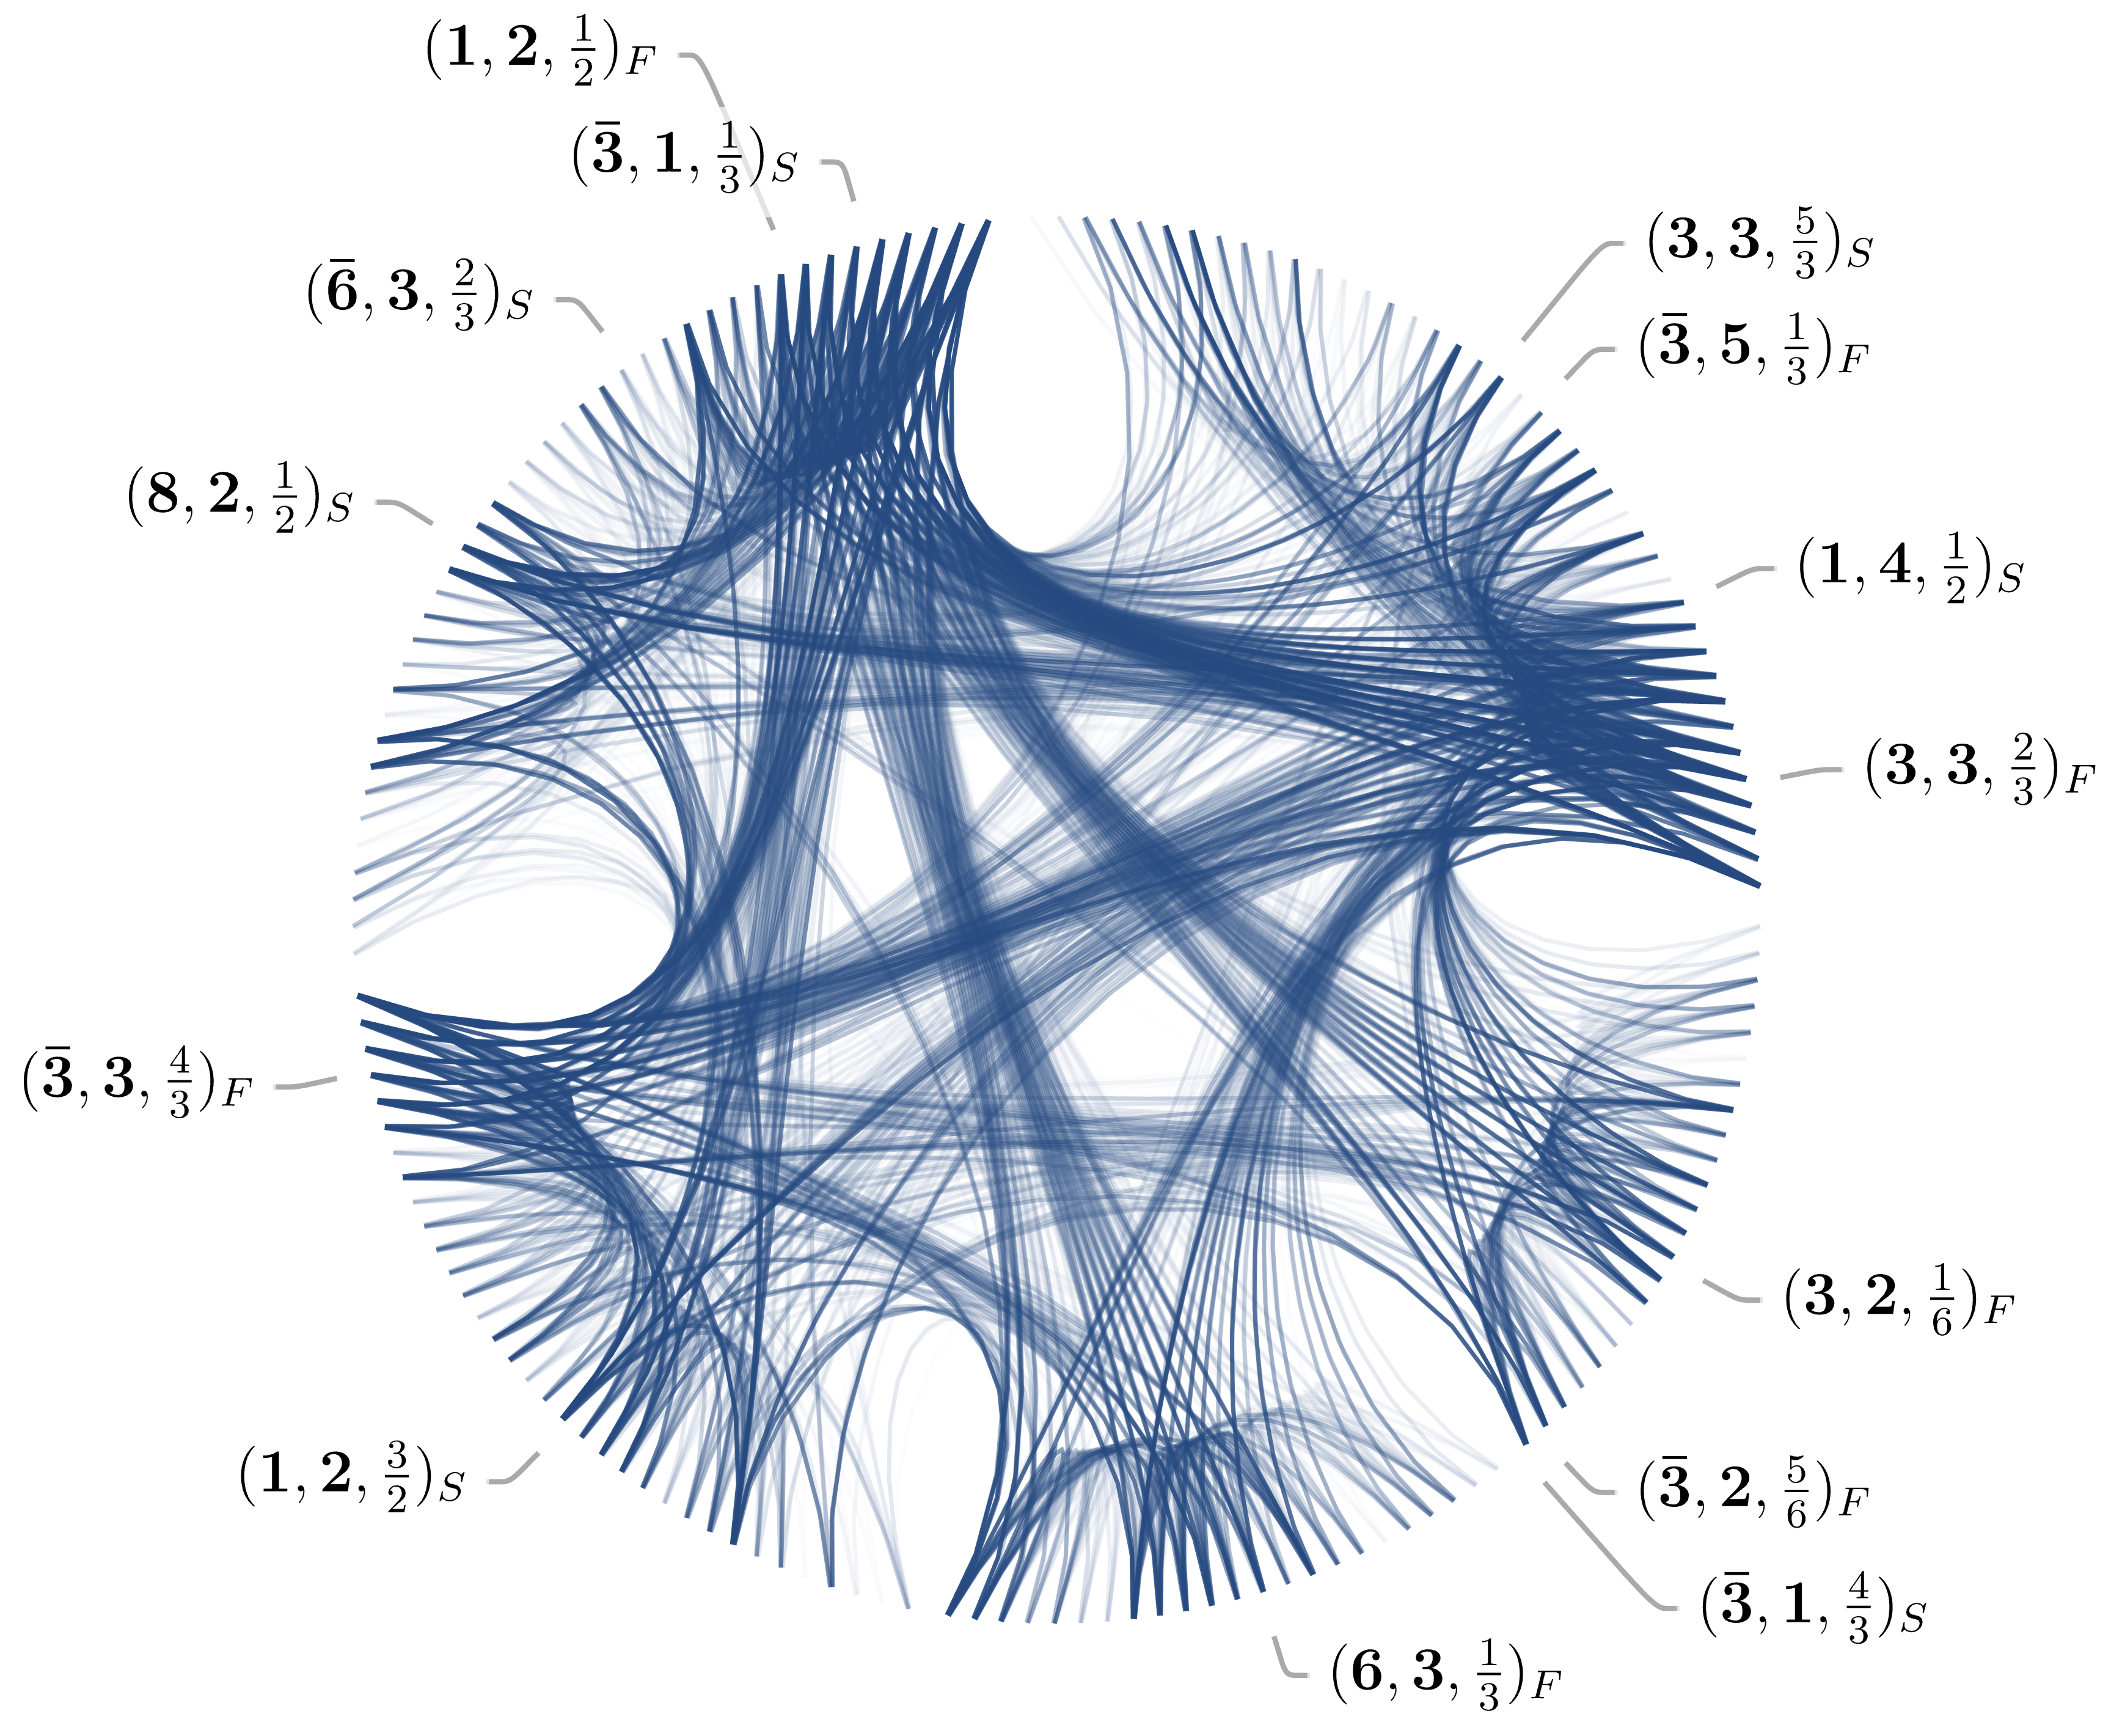
\includegraphics[width=0.8\textwidth]{connectionGraph.png}
  \caption[The graph is a representation of the connectivity between exotic
  fields in the neutrino-mass models.]{The graph is a representation of the
    connectivity between exotic fields in the neutrino-mass models. Each node
    represents an exotic field and edges connect fields featuring together in a
    neutrino-mass model. The colour is an indication of the weight of the edge,
    \textit{i.e.} the number of times the two nodes appear in models together.
    The graph is clustered into roughly five communities within which there are
    many mutual connections. Only a handful of node labels are shown.}
  \label{fig:ch2-model-graph}
\end{figure}

\subsection{Example models}
\label{sec:ch2-example-models}

In this section we present some example neutrino-mass models, illustrating use
cases of the model database, aspects to be careful of in its use, and
representative features of the novel models derived from dimension-eleven and
dimension-nine operators.

\subsubsection{Simple models at the TeV scale}
\label{sec:ch2-simple-models}

We are particularly interested in models that are simple, in the sense that they
involve few exotic fields, and testable, in that they predict new physics at
currently or nearly accessible energy ranges. We query our model database to
return models featuring three fields or fewer with the estimated upper bound on
the new-physics scale required to be between \SI{700}{\GeV} and \SI{100}{\TeV}.
The results of the query are presented in Table~\ref{tab:ch2-simple-models}. There
are twelve\footnote{We note that there are technically more models: those for
  which the colour-sextet fields in Table~\ref{tab:ch2-simple-models} are replaced
  with colour triplets, with a corresponding baryon-number assignment such that
  the same interactions as the sextet are picked out.} models listed, only one
of which has explicitly appeared before in the literature to our knowledge: the
completion of $\mathcal{O}_{8}$ discussed in Sec.~\ref{sec:ch2-modelsoverview}. It
is interesting to note that the scalar leptoquark\footnote{We mention
  parenthetically that although this leptoquark does not possess diquark
  couplings, baryon-number violation does occur through a term in the scalar
  potential. The leading-order contribution is through a dimension-ten operator
  mediating $p \to \pi^{+}\pi^{+} e^{-} \nu \nu$~\cite{Arnold:2012sd}.}
$\Pi_{1} \sim (\mathbf{3}, \mathbf{2}, \tfrac{1}{6})_{S}$ appears in almost
every model listed in the table. This suggests that our general analysis of the
frequency of fields appearing in the completions in
Sec.~\ref{sec:ch2-modelsoverview} may look different if specific selection criteria
are placed on the data. We have checked the full Lagrangians implied by the
field content of each model and found that seven of the models listed in the
table imply the generation of the Weinberg operator through heavy loops. We
emphasise that these non-genuine completions are potentially interesting and new
radiative models, although the neutrino self-energy diagram will look different
to that implied by the closure of the tree-level graph from which the model was
derived. This means that the bound on the implied new-physics scale is in
general higher than that suggested by the closure of the original operator. In
this class are all of the models for which the upper bound on the new-physics
scale is larger than \SI{15}{\TeV}. This means that there are only five models
in our database with fewer than four fields for which the upper bound on
$\Lambda$ is between \SI{700}{\GeV} and \SI{100}{\TeV}, and they all predict new
physics below \SI{15}{\TeV}. In the following we present two example models from
the table:
\begin{enumerate}
  \item We look at one of the models---the one derived from
    $\mathcal{O}_{62b}$---that generates the Weinberg operator through a heavy
    loop. We intend this to be an example of how this phenomenon can appear and
    how it is easy to diagnose in some cases.
  \item We present a brief study of the implications for neutrino mass implied
    by the model given in the last row.
\end{enumerate}

\begin{table}
  \centering
  \bgroup
  \def\arraystretch{1.3}
  \begin{tabular}{cclc}
    \toprule
    Field content & Operators & $\Lambda~[\TeV]$ & Dominant? \\
    \midrule
    $(\mathbf{3}, \mathbf{2}, \tfrac{1}{6})_{S}$, $(\mathbf{3}, \mathbf{2}, \tfrac{7}{6})_{F}$ & $8$, $D15$ & 15 & Y \\
    $(\mathbf{1}, \mathbf{2}, \tfrac{1}{2})_{F}$, $(\mathbf{1}, \mathbf{1}, 1)_{S}$, $(\mathbf{1}, \mathbf{2}, \tfrac{3}{2})_{S}$ & $62b$ & 16 & N \\
    $(\mathbf{\bar{3}}, \mathbf{2}, \tfrac{5}{6})_{S}$, $(\mathbf{3}, \mathbf{2}, \tfrac{1}{6})_{F}$, $(\mathbf{3}, \mathbf{2}, \tfrac{1}{6})_{S}$ & $8^{\prime}$ & 1 & N \\
    $(\mathbf{\bar{3}}, \mathbf{1}, \tfrac{1}{3})_{S}$, $(\mathbf{\bar{6}}, \mathbf{2}, \tfrac{1}{6})_{S}$, $(\mathbf{3}, \mathbf{2}, \tfrac{1}{6})_{F}$ & $24f$ & 89 & N \\
    $(\mathbf{\bar{3}}, \mathbf{3}, \tfrac{1}{3})_{F}$, $(\mathbf{\bar{6}}, \mathbf{2}, \tfrac{1}{6})_{S}$, $(\mathbf{3}, \mathbf{2}, \tfrac{1}{6})_{S}$ & $24d$ & 89 & N \\
    $(\mathbf{\bar{3}}, \mathbf{2}, \tfrac{5}{6})_{S}$, $(\mathbf{1}, \mathbf{2}, \tfrac{3}{2})_{F}$, $(\mathbf{3}, \mathbf{2}, \tfrac{1}{6})_{S}$ & $8^{\prime}$ & 1 & N \\
    $(\mathbf{\bar{3}}, \mathbf{3}, \tfrac{1}{3})_{F}$, $(\mathbf{\bar{6}}, \mathbf{4}, \tfrac{1}{6})_{S}$, $(\mathbf{3}, \mathbf{2}, \tfrac{1}{6})_{S}$ & $24f$ & 89 & N \\
    $(\mathbf{\bar{3}}, \mathbf{1}, \tfrac{1}{3})_{F}$, $(\mathbf{\bar{6}}, \mathbf{2}, \tfrac{1}{6})_{S}$, $(\mathbf{3}, \mathbf{2}, \tfrac{1}{6})_{S}$ & $24d$ & 89 & N \\
    $(\mathbf{\bar{6}}, \mathbf{2}, \tfrac{7}{6})_{F}$, $(\mathbf{8}, \mathbf{2}, \tfrac{1}{2})_{S}$, $(\mathbf{3}, \mathbf{2}, \tfrac{1}{6})_{S}$ & $20$ & 0.8 & Y \\
    $(\mathbf{6}, \mathbf{1}, \tfrac{4}{3})_{S}$, $(\mathbf{6}, \mathbf{1}, \tfrac{1}{3})_{F}$, $(\mathbf{3}, \mathbf{2}, \tfrac{1}{6})_{S}$ & $20$ & 0.8 & Y \\
    $(\mathbf{6}, \mathbf{2}, \tfrac{5}{6})_{S}$, $(\mathbf{3}, \mathbf{2}, \tfrac{1}{6})_{F}$, $(\mathbf{3}, \mathbf{2}, \tfrac{1}{6})_{S}$ & $50a,b$ & 10 & Y \\
    $(\mathbf{\bar{6}}, \mathbf{2}, \tfrac{1}{6})_{S}$, $(\mathbf{\bar{3}}, \mathbf{2}, \tfrac{5}{6})_{F}$, $(\mathbf{3}, \mathbf{2}, \tfrac{1}{6})_{S}$ & $50a,b$ & 10 & Y \\
    \bottomrule
  \end{tabular}
  \egroup
  \caption[The table shows the models in our filtered list that contain fewer
  than four fields with the estimate of the upper-bound on the new-physics scale
  $\Lambda$ in the range $\SI{700}{\GeV} < \Lambda < \SI{100}{\TeV}$.]{The table
    shows the models in our filtered list that contain fewer than four fields
    with the estimate of the upper-bound on the new-physics scale $\Lambda$ in
    the range $\SI{700}{\GeV} < \Lambda < \SI{100}{\TeV}$. Models containing
    colour sextet fields can be replaced with the corresponding colour-triplet
    fields with a different baryon-number assignment. The fields and models are
    listed in no special order. The scalar leptoquark
    $\Pi_{1} \sim (\mathbf{3}, \mathbf{2}, \tfrac{1}{6})$ appears in almost all
    of the models listed. Completions marked as non-dominant may be viable and
    interesting neutrino-mass models, but the main contribution to the neutrino
    mass does not come from the closure of the tree-level diagram from which the
    particle content was derived. This means, among other things, that the upper
    bound on the scale of the new physics associated with the model will differ
    to that presented here.}
  \label{tab:ch2-simple-models}
\end{table}

\paragraph{Model derived from $\mathcal{O}_{62b}$} The model derived from
$\mathcal{O}_{62b}$ is especially simple since it does not require the
imposition of $\mathrm{U}(1)_{B}$. The exotic fields introduced are
$\Delta_{1} \sim (\mathbf{1}, \mathbf{2}, \tfrac{1}{2})_{F}$,
$\mathcal{S}_{1} \sim (\mathbf{1}, \mathbf{1}, 1)_{S}$ and
$\chi \sim (\mathbf{1}, \mathbf{2}, \tfrac{3}{2})_{S}$. The additional
interaction Lagrangian necessary to generate $\mathcal{O}_{62b}$ at tree level
is $\Delta \mathscr{L} = \mathscr{L}_{Y} - \mathcal{V}$, with
\begin{align}
  - \mathscr{L}_{Y} &= m_{\Delta_{1}} \bar{\Delta}_{1} \Delta_{1} + x_{[rs]} L^{i}_{r} L^{j}_{s} \mathcal{S}_{1}\epsilon_{ij} + y_{r} \bar{e}_{r} \bar{\Delta}_{1}^{i} \tilde{H}^{j} \epsilon_{ij} + z_{r}\bar{e}_{r} \tilde{\chi}^{i} \Delta_{1}^{j} \epsilon_{ij} \ , \\
  \mathcal{V} &= m_{\mathcal{S}_{1}}^{2} \mathcal{S}_{1}^{\dagger} \mathcal{S}_{1} + m_{\chi}^{2} \chi^{\dagger} \chi + w H^{i} \chi^{j} \mathcal{S}^{\dagger}_{1} \mathcal{S}^{\dagger}_{1} \epsilon_{ij} \ .
\end{align}
This implies that the neutrino-mass mechanism depends on 13 new parameters: nine
Yukawa couplings, $w$ and the three masses; although there are a much larger
number of terms present in the full Lagrangian of the model. Importantly, one of
these is
$x^{\prime}_{r} L_{r}^{i} \bar{\Delta}^{j}_{1} \mathcal{S}_{1} \epsilon_{ij}$,
which we now show is sufficient to generate the Weinberg operator through a
two-loop diagram containing one heavy loop.

The tree-level completion diagram and the neutrino-mass diagram relevant to the
model are shown in Fig.~\ref{fig:ch2-leptonic-model-diagrams}. There are two- and
three-loop neutrino self-energies, where the three-loop models arise by
connecting the $H$ and $H^{\dagger}$ lines in
Fig.~\ref{fig:ch2-leptonic-model-neutrinomass} in all possible ways. In this case,
the first part of the fermion line (highlighted in
Fig.~\ref{fig:ch2-leptonic-model-neutrinomass}) can be replaced with the
aforementioned $L\bar{\Delta}_{1}\mathcal{S}_{1}$ vertex so that the left loop
contains only $\mathcal{S}_{1}$, $\chi$ and the Dirac fermion
$\Delta_{1} + \bar{\Delta}_{1}^{\dagger}$. (It can also be noticed from the
tree-level opening in Fig.~\ref{fig:ch2-leptonic-model-treelevel} that the
$\Delta_{1}$ line can be connected directly to one of the $LL\mathcal{S}_{1}$
vertices, giving rise to a loop-level completion of $\mathcal{O}_{2}$.) This
heavy-loop neutrino-mass diagram, although interesting in its own right,
predicts a different mass-scale for the exotic fields (roughly \SI{e6}{\TeV}),
and a different structure for the neutrino-mass matrix.

\begin{figure}[t]
  \centering
  \subcaptionbox{\label{fig:ch2-leptonic-model-treelevel}}{
    \includegraphics[width=0.35\linewidth]{leptonic_example_treelevel.pdf}
  }
  \subcaptionbox{\label{fig:ch2-leptonic-model-neutrinomass}}{
    \includegraphics[width=0.6\linewidth]{leptonic_example_neutrinomass.pdf}
  }
  \caption[(a) The furnishing of the tree-level topology, labelled $2s6f_4$ in
  our scheme, that generates $\mathcal{O}_{62b}$ at tree level. (b) The neutrino
  self-energy diagram relevant to the non-genuine completion of
  $\mathcal{O}_{62b}$.]{(a) The furnishing of the tree-level topology, labelled
    $2s6f_4$ in our scheme, that generates $\mathcal{O}_{62b}$ at tree level.
    The interactions allowed in the theory are such that the $\Delta_{1}$ line
    can be connected straight into one of the $LL\mathcal{S}_{1}$ vertices in
    place of an $L$, leading to a loop-level completion of $\mathcal{O}_{2}$.
    (b) The neutrino self-energy diagram relevant to the non-genuine completion
    of $\mathcal{O}_{62b}$. It is clear that this diagram does not represent the
    dominant contribution to the neutrino mass, since the highlighted collection
    of fields can be replaced with the interaction
    $\bar{\Delta}_{1} L \mathcal{S}_{1}$. This leads to a diagram with heavy
    loop involving $\Delta_{1}$, $\chi$ and $\mathcal{S}_{1}$, which dominates
    the neutrino masses. In both cases, the relevant topology is CLBZ-7 in the
    classification of Ref.~\cite{Sierra:2014rxa}.}
  \label{fig:ch2-leptonic-model-diagrams}
\end{figure}

\paragraph{A genuine low-scale model} Below we present a brief exploration of
the model derived from $\mathcal{O}_{50}$ that contains the exotic fields
$\phi \sim (\mathbf{6}, \mathbf{2}, -\tfrac{1}{6})_{F}$,
$\Pi_{1} \sim (\mathbf{3}, \mathbf{2}, \tfrac{1}{6})_{S}$ and
$Q_{5} \sim (\mathbf{3}, \mathbf{2}, -\tfrac{5}{6})_{F}$. The estimate for the
neutrino mass derived from the operator closure suggests this model's exotic
particle content should live roughly below \SI{10}{\TeV}. The corresponding
$\Delta L = 2$ Lagrangian we write again as
$\Delta \mathscr{L} = \mathscr{L}_{Y} - \mathcal{V}$, with
\begin{align}
  -\mathscr{L}_{Y} &= x_{rs} L^{i}_{r} \bar{d}_{sa} \Pi_{1}^{aj} \epsilon_{ij} + y_{r} \phi^{\{ab\}i} \bar{u}_{ra} \bar{Q}^{j}_{5 b} \epsilon_{ij} + z_{r} \bar{d}_{ra} H^{i} Q^{aj}_{5} \epsilon_{ij} + \text{h.c.} \label{eq:ch2-low-scale-yuks} \\
  \mathcal{V} &= \lambda \tilde{\Pi}_{1a}^{i} \tilde{\Pi}_{1b}^{j} \phi^{\{ab\}k} H^{l} (\epsilon_{ik}\epsilon_{jl} + \epsilon_{il}\epsilon_{jk}) \ .
\end{align}
We note that $\mathrm{U}(1)_{B}$ must be imposed on the Lagrangian to prevent
terms like $\Pi^{3}_{1} H^{\dagger}$, $|\phi|^{2}\phi^{\dagger}\Pi_{1}$ and
$|\Pi_{1}|^{2} \Pi_{1} \phi$ that destabilise the proton in the presence of the
Yukawa interactions of Eq.~\eqref{eq:ch2-low-scale-yuks}. The field $\phi$ only
couples to SM fermions together with $Q_{5}$ in this model, and so it generates
no dimension-six operators at tree level. The completion graph and one of the
neutrino self-energy diagrams are shown in Fig.~\ref{fig:ch2-lowscale-example}. The
tree-level topology is again $2s6f_{4}$, and the neutrino masses are realised at
three and four loops, with the additional loop arising from the connection of an
$H$ and $H^{\dagger}$. One of the loops involves a $W$ boson, and so the diagram
does not fit into existing topological classifications. The three-loop diagram
is similar to the topology $D_{9}^{M}$ of Ref.~\cite{Cepedello:2018rfh}, with
one of the scalar lines replaced with a vector boson. The $W$ boson line must
connect to $Q$ in the diagram, but could end on any field with non-trivial
$\mathrm{SU}(2)_{L}$ charge. The connection to the $L$ line is shown, since the
loop integral then depends on leptonic flavour indices, which can change the
structure of the neutrino-mass matrix. There are also several ways of connecting
the Higgs lines and only one combination is shown in the figure. The four-loop
diagrams will be the dominant contribution to the neutrino masses for exotic
fields above $4 \pi v \approx \SI{2}{\TeV}$.

The neutrino-mass matrix in this model can be estimated as
\begin{equation}
  [\mathbf{m}_{\nu}]_{rs} = \frac{\lambda g^{2}}{(16\pi^{2})^{3}} \left( \frac{v^{2}}{\Lambda^{2}} + \frac{1}{16\pi^{2}}\right) \frac{1}{\Lambda}\sum_{t,u,v} x_{rt} z^{*}_{t} y^{*}_{u} [\mathbf{m}_{u}]_{u} V_{uv} [\mathbf{m}_{d}]_{v} x_{sv} I_{rstuv} + (r \leftrightarrow s) \ ,
\end{equation}
where the $V_{rs}$ are CKM matrix elements, $\Lambda$ is the generic UV scale,
and $I_{rstuv}$ is the loop function. The dependence on the masses of the up-
and down-type quarks implies that the largest contributions to the neutrino
masses will come from loops containing top and bottom quarks. If the parameters
$y_{1,2}$, $x_{r1}$ and $x_{r2}$ play no significant role in the physics of
neutrino mass, then the matrix will have rank 1 if the loop function carries no
leptonic flavour indices. It may be the case that an additional generation of
$Q_{5}$, $\phi$ or $\Pi_{7}$ is therefore required for the model to successfully
reproduce the measured pattern of neutrino masses and mixings.

\begin{figure}[t]
  \centering
  \subcaptionbox{\label{fig:ch2-lowscale-model-treelevel}}{
    \includegraphics[width=0.35\linewidth]{lowscale_example_treelevel.pdf}
  }
  \subcaptionbox{\label{fig:ch2-lowscale-model-neutrinomass}}{
    \includegraphics[width=0.6\linewidth]{lowscale_example_neutrinomass.pdf}
  }
  \caption[(a) The tree-level completion diagram for the model derived from
  exploding $\mathcal{O}_{50}$ and discussed in the main text. (b) One of the
  neutrino-mass diagrams relevant to the model derived from
  $\mathcal{O}_{50}$.]{(a) The tree-level completion diagram for the model
    derived from exploding $\mathcal{O}_{50}$ and discussed in the main text.
    The topology is $2s6f_{4}$ in our classification scheme. The closure
    involves an arrow-preserving loop connecting the $\bar{d}^{\dagger}$ to one
    of the $\bar{d}$ lines, and the $W$-boson closure motif discussed in
    Sec.~\ref{sec:ch2-operator-closures}. (b) One of the neutrino-mass diagrams
    relevant to the model derived from $\mathcal{O}_{50}$. There is a three-loop
    diagram with the $H$ line broken into an $H^{\dagger}, H$ pair that
    generates the dimension-seven generalised Weinberg operator. The four-loop
    diagrams all involve connecting the $H^{\dagger}$ to each of the three $H$
    legs in the diagram. There are also multiple places the $W$ could end in the
    diagram, although it must couple to the $Q$ line. The four-loop diagrams
    will give larger contributions to the neutrino mass than the three-loop
    diagrams for $\Lambda \gtrsim \SI{2}{\TeV}$.}
  \label{fig:ch2-lowscale-example}
\end{figure}

\subsubsection{A model derived from a derivative operator}

We move on to discuss a model generating the single-derivative dimension-nine
operators $\mathcal{O}_{D10a,b,c}$. The estimated upper-bound on the exotic
scale is close to \SI{1.5e3}{\TeV} in this case. The model contains the fields
$\rho \sim (\mathbf{1}, \mathbf{2}, \tfrac{3}{2})_{S}$,
$Q_{5} \sim (\mathbf{3}, \mathbf{2}, \tfrac{5}{6})_{F}$ and
$\Sigma_{1} \sim (\mathbf{1}, \mathbf{3}, 1)_{F}$. Such two-fermion--one-scalar
models are unique to completions of single-derivative operators at dimension
nine.

The part of the Lagrangian relevant to lepton-number violation is
\begin{equation}
  - \Delta \mathscr{L} = x_{r} L_{r}^{i} \Sigma_{1}^{\{jk\}} H^{\dagger}_{k} \epsilon_{ij} + y_{r} L_{r}^{i} \rho^{j} \bar{\Sigma}_{1}^{\{kl\}}\epsilon_{ik}\epsilon_{jl} + z_{r} \bar{d}_{ra} H^{i} Q^{aj}_{5} \epsilon_{ij} + w_{r} \bar{u}_{ra} \rho^{i} Q_{5}^{aj} \epsilon_{ij} + \text{h.c.}
\end{equation}
The only additions to the scalar potential are the expected $|\rho|^{2}|H|^{2}$
and $|\rho|^{4}$ terms, and these play no role in the lepton-number violation.
Notably, there are no Yukawa couplings involving $\bar{Q}_{5}$, and the field
$\rho$ generates no dimension-six operators at tree-level, since the naively
expected coupling $H^{i}H^{j}H^{k}\rho_{k} \epsilon_{ij}$ vanishes. The model
also has the nice feature that no baryon-number violating interactions are
present.

The tree-level completion diagram and one of the neutrino-mass diagrams are
shown in Fig.~\ref{fig:ch2-derivative-example-diagrams}. The completion diagram has
topology $2s4f_{8}$, which requires one of the heavy fermions to have an
arrow-preserving propagator. The neutrino-mass diagram shown is
cocktail-like~\cite{Gustafsson:2012vj}, although there are also two-loop diagrams generating
$\mathcal{O}_{1}^{\prime}$ at the low scale, as well as other diagrams with the
$W$ and $H$ lines in different places. The topology of the neutrino self-energy
diagram is similar to $D^{M}_{15}$ in Ref.~\cite{Cepedello:2018rfh}.

The flavour structure of the neutrino-mass matrix has the approximate form
\begin{equation}
  [\mathbf{m}_{\nu}]_{rs} = \frac{g^{2}}{(16\pi^{2})^{3}} \frac{1}{\Lambda} \sum_{t,u} y_{r} x_{s} w^{*}_{t} z_{t} [\mathbf{m}_{d}]_{t} V_{ut} [\mathbf{m}_{u}]_{u} I_{rstu} + (r \leftrightarrow s) \ .
\end{equation}
The dependence on the up- and down-type mass matrices, as in the example
presented in Sec.~\ref{sec:ch2-simple-models}, means that the couplings $w_{1,2}$
and $z_{1,2}$ will not play an important role in generating the observed pattern
of neutrino masses and mixings. In this case the matrix has at least rank 2,
even if the leptonic-flavour structure of the loop integrals $I_{rstu}$ is flat.
Thus, the structure of the neutrino masses and mixing parameters emerges mostly
from the six parameters $x_{r}$ and $y_{r}$.

\begin{figure}[t]
  \centering
  \subcaptionbox{\label{fig:ch2-derivative-example-treelevel}}{
    \includegraphics[width=0.5\linewidth]{derivative_example_treelevel.pdf}
  }
  \subcaptionbox{\label{fig:ch2-derivative-example-neutrinomass}}{
    \includegraphics[width=0.4\linewidth]{derivative_example_neutrinomass.pdf}
  }
  \caption[(a) The tree-level completion diagram for the model that generates
  the single-derivative operators $\mathcal{O}_{D10,a,b,c}$ and discussed in the
  main text. (b) One of the neutrino-mass diagrams relevant to the model
  generating $\mathcal{O}_{D10a,b,c}$.]{(a) The tree-level completion diagram
    for the model that generates the single-derivative operators
    $\mathcal{O}_{D10,a,b,c}$ and discussed in the main text. The topology is
    $2s4f_{8}$ in our classification scheme. This class of topologies is only
    relevant to single-derivative operators, and contains an arrow-preserving
    fermion propagator, that of $Q_{5}$ in the diagram. The closure of the
    diagram involves a $W$-boson loop, similar to that required in
    Fig.~\ref{fig:ch2-lowscale-example}. (b) One of the neutrino-mass diagrams
    relevant to the model generating $\mathcal{O}_{D10a,b,c}$. The diagram
    generates the Weinberg operator as drawn, but additional diagrams exist with
    the central $H$ line cut into an $H,H^{\dagger}$ pair that generate
    $\mathcal{O}^{\prime}_{1}$ instead. These diagrams will only be relevant for
    exotic masses less than about $\SI{2}{\TeV}$. Additional three-loop diagrams
    exist in which the Higgs coming from the $\Sigma_{1}LH^{\dagger}$
    interaction loops into any of the other external $H$ fields. The $W$ boson
    must connect to the $Q$ line, but could end on any other field with
    non-trivial $\mathrm{SU}(2)_{L}$ charge. The topology is
    cocktail-like~\cite{Gustafsson:2012vj}, and resembles $D^{M}_{15}$ in
    Ref.~\cite{Cepedello:2018rfh}.}
  \label{fig:ch2-derivative-example-diagrams}
\end{figure}

\subsubsection{A model of neutrino mass and the flavour anomalies}
\label{sec:ch2-anomalies-mv}

Here we present a model designed specifically to generate a particular set of
dimension-six operators. The example is motivated by the flavour anomalies,
discussed in detail in Sec.~\ref{sec:ch1-flavour-anomalies}. In the following we
adhere to the conventions\footnote{These can be accessed easily at
  \url{https://flav-io.github.io/docs/operators.html}.} of
Ref.~\cite{Aebischer:2017ugx} relevant to the Warsaw basis for the SMEFT and the
\textsf{flavio} basis~\cite{Straub:2018kue} for the Weak Effective Theory (WET).
The leptoquarks
$\omega_{1} \sim (\mathbf{\bar{3}}, \mathbf{1}, \tfrac{1}{3})_{S}$ and
$\Pi_{7} \sim (\mathbf{3}, \mathbf{2}, \tfrac{7}{6})_{S}$ can provide an
explanation of the anomalies in $R_{D^{(*)}}$ with contributions to the SMEFT
operators
\begin{align}
  \label{eq:ch2-rdrdstar-relation}
  [C_{lequ}^{(1)}]_{3332} = \begin{cases}
    - 4 [C_{lequ}^{(3)}]_{3332} &\text{for } \omega_{1} \\
    4 [C_{lequ}^{(3)}]_{3332}  &\text{for } \Pi_{7} \\
  \end{cases} \ ,
\end{align}
since they have Yukawa couplings to left- and right-handed SM fields. [We note
that Eq.~\eqref{eq:ch2-rdrdstar-relation} holds at the high scale, and the relation
between the operators is altered by running.] The Yukawa terms are
\begin{align}
  - \mathcal{L}_{\omega_{1}} &= f_{rs} L_{r} Q_{s} \omega_{1} + g_{rs} \bar{e}^{\dagger}_{r} \bar{u}^{\dagger}_{s} \omega_{1} + \text{h.c.} \label{eq:ch2-omega1-coup} \\
  - \mathcal{L}_{\Pi_{7}} &= x_{rs} L_{r} \bar{u}_{s} \Pi_{7} + y_{rs} \bar{e}^{\dagger}_{r} Q^{\dagger}_{s} \Pi_{7} + \text{h.c.} \label{eq:ch2-pi7-coup}
\end{align}
and these imply
\begin{align}
  \label{eq:ch2-omega1-pi7-clequ}
  [C_{lequ}^{(1)}]_{3332} = \begin{cases}
    \dfrac{f_{33} g_{32}^{*}}{2 m_{\omega_{1}}^{2}} &\text{for } \omega_{1} \\
    \dfrac{x_{32}^{*}y_{33}}{2 m_{\Pi_{7}}^{2}} &\text{for } \Pi_{7} \\
  \end{cases}
\end{align}
at tree level. A satisfactory explanation of $R_{D^{(*)}}$ requires
$\mathcal{O}(1)$ couplings, \textit{e.g.}~\cite{Cai:2017wry, Popov:2019tyc}, and
for $\Pi_{7}$ fits are consistent with the operator coefficient being purely
imaginary, \textit{e.g.}~\cite{Angelescu:2018tyl}.

The $b \to s$ data can be explained by the tree-level exchange of the leptoquark
$\zeta \sim (\mathbf{\bar{3}}, \mathbf{3}, \tfrac{1}{3})_{S}$, which generates
\begin{equation}
  [C_{lq}^{(1)}]_{2223} = 3 [C_{lq}^{(3)}]_{2223} \ ,
\end{equation}
relevant for the neutral-current anomalies. We saw in
Sec.~\ref{sec:ch1-neutral-current-anomalies} that fits are performed to the
four-fermion operators $C^{bs\mu\mu}_{9}$ and $C^{bs\mu\mu}_{10}$ in the WET.
For the $b \to s \ell \ell$ data, a good fit is given
for~\cite{Aebischer:2019mlg}
\begin{equation}
  C_{9}^{bs\mu\mu} = - C_{10}^{bs\mu\mu} = \frac{1}{2} \left(  V_{tb} V_{ts}^{*} \frac{e^{2}}{16\pi^{2}} \frac{4 G_{F}}{\sqrt{2}} \right)^{-1} \left[ C_{lq}^{(1)} + C_{lq}^{(3)} \right]_{2232} \approx -0.5 \ ,
\end{equation}
where $C_{9,10}^{bs\mu\mu}$ are referred to simply as $C_{9,10}$ in
Sec.~\ref{sec:ch1-flavour-anomalies}.

It was pointed out in Ref.~\cite{Aebischer:2019mlg} that there exists a mild
tension between the fit to $R_{K^{(*)}}$ and the other anomalous $b \to s$ data,
which can be reconciled with an additional LFU contribution to
$C_{9}^{bs\ell\ell}$ such that
\begin{equation}
  C_{9}^{bs\mu\mu} \approx -0.44\quad \text{ and }\quad C_{9}^{bs\ell\ell} \approx -0.5 \ ,
\end{equation}
for $\ell \in \{e, \mu, \tau\}$. A potential source of this universal
contribution to $C_{9}$ is new physics in four-quark operators
like~\cite{Aebischer:2019mlg}
\begin{equation}
  \label{eq:ch2-ouq}
  [\mathcal{O}_{qu}^{(1)}]_{2322} = (\bar{Q}_{2} \gamma_{\mu} Q_{3}) (\bar{u}_{2} \gamma^{\mu} \bar{u}_{2}) \ ,
\end{equation}
which can be generated, for example, by
$\Phi \sim (\mathbf{8}, \mathbf{2}, \tfrac{1}{2})_{S}$. The relevant Yukawa terms are
\begin{equation}
  \label{eq:ch2-phi-yuks}
  - \mathscr{L}_{\Phi} = w_{rs} Q_{r}^{ai} \bar{u}_{sb} \Phi^{bj}_{\ a} \epsilon_{ij} + \text{h.c.}
\end{equation}
and a contribution of about the right size to $C_{9}^{bs\ell\ell}$ can be
generated while avoiding dijet exclusion bounds from the LHC for
$m_{\Phi} \sim \SI{2}{\TeV}$ and
$|w_{22}|, |w_{32}| \sim 1$~\cite{Aebischer:2019mlg}.

We construct a UV model that contains $\zeta$ and $\Phi$ as well as one of
$\omega_{1}$ or $\Pi_{7}$ in an attempt to incorporate this explanation into a
model of neutrino mass. We emphasise that our goal here is not to present the
most elegant or motivated model of neutrino mass and the flavour anomalies, but
rather to show that our database can be used to motivate complex models with a
specific structure.

We query the filtered model database for neutrino-mass models that contain the
interactions $Q \bar{u} \Phi$, needed to generate $\mathcal{O}_{qu}^{(1)}$;
$LQ\zeta$, needed to generate $C_{9}^{bs\mu\mu} = -C_{10}^{bs\mu\mu}$; and one
of $\omega_{1}$ or $\Pi_{7}$, required to explain $R_{D^{(*)}}$. Our query
returns a number of models, and we choose one to study briefly below. We note
that none of the models involve the leptoquark $\omega_{1}$, and none feature
the interaction $\bar{e}^{\dagger} Q^{\dagger} \Pi_{7}$, implying some freedom
in the explanation of $R_{D^{(*)}}$ since the couplings $y_{rs}$ of
Eqs.~\eqref{eq:ch2-pi7-coup} and \eqref{eq:ch2-omega1-pi7-clequ} will be
unrelated\footnote{Expanding our search criteria, we find no viable models in
  the database in which both sets of couplings presented in
  Eqs.~\eqref{eq:ch2-omega1-coup} and \eqref{eq:ch2-pi7-coup} feature. This can be
  understood in the following way. Any neutrino self-energy diagram containing
  both couplings will also imply another where
  $\bar{e}^{\dagger} \bar{u}^\dagger \omega_{1}$ or
  $\bar{e}^{\dagger} Q^{\dagger} \Pi_{7}$ is replaced with the corresponding
  coupling to $L$, which contains a neutrino field. This generally gives a
  larger contribution to the neutrino mass, since the closure of the diagram
  containing the $\bar{e}$ will involve an additional loop with a $W$ boson.
  Thus, diagrams with both sets of Yukawa interactions to SM fermions relevant
  to $\omega_{1}$ and $\Pi_{7}$ are likely to be removed by our filtering
  procedure. We note that, after studying the unfiltered list of models, we find
  that some models can be engineered so that a sizeable (but not dominant)
  contribution to the neutrino masses does come from such diagrams involving
  both sets of leptoquark--fermion Yukawa couplings.} to the neutrino mass.

The model contains the additional fields $\Phi$, $\zeta$, $\Pi_{7}$ and
$\eta \sim (\mathbf{8}, \mathbf{1}, 1)_{S}$, necessary for lepton-number
violation. It generates $\mathcal{O}_{29b}$, which implies an upper bound on the
new-physics scale of roughly $\SI{e7}{\TeV}$. The additional piece of the
Lagrangian is $\Delta \mathscr{L} = \mathscr{L}_{Y} - \mathcal{V}$, with
\begin{align}
  -\mathscr{L}_{Y} &= x_{rs} L^{i}_{r}\bar{u}_{sa} \Pi^{ja}_{7} \epsilon_{ij} +  y_{rs} \bar{e}^{\dagger}_{r} Q_{sai}^{\dagger} \Pi^{ai}_{7} + z_{rs}L^{i}_{r} Q^{ja}_{s} \zeta_{a}^{\{kl\}} \epsilon_{ik} \epsilon_{jl} + w_{rs} Q^{ai}_{r} \bar{u}_{sb} \Phi^{bj}_{\ a} \epsilon_{ij}  + \text{h.c.} \label{eq:ch2-flav-anom-yuks} \\
  \mathcal{V} &= \kappa H^{i} \Phi^{a j}_{\ b} \eta^{\dagger b}_{\ \ a} \epsilon_{ij} + \lambda H^{i} \eta^{a}_{\ b} \tilde{\Pi}^{j}_{7a} \tilde{\zeta}^{b \{kl\}} \epsilon_{ik}\epsilon_{jl} + \text{h.c.} + \cdots \ ,
\end{align}
where we have only shown the part of the scalar potential relevant to
lepton-number violation in this model, since the full expression contains a
large number of terms. The leptoquark $\zeta$ has a diquark coupling which we
forbid by imposing $\mathrm{U}(1)_{B}$ on the Lagrangian, assigning baryon
numbers of $-\tfrac{1}{3}$ and $\tfrac{1}{3}$ to $\zeta$ and $\Pi_{7}$,
respectively. (All other exotic fields have $B = 0$.) The model contains 33 free
parameters, although not all of them are necessary to address the flavour
anomalies and generate viable neutrino masses.

The tree-level completion diagram and the neutrino self-energy diagram are shown
in Fig.~\ref{fig:ch2-flavour-anomalies-model-diagrams}. The neutrino mass arises at
two loops, and the topology has the feature that no fermion propagators are
arrow-violating. This implies that the neutrino masses are not proportional to
any SM-fermion masses. This feature has been studied before in the context of a
specific UV model in Ref.~\cite{Gargalionis:2019drk}. The phenomenon is
particular to models derived from operators whose closures feature
arrow-preserving loops, as discussed in Sec.~\ref{sec:ch2-operator-closures}. From a
model-building perspective, one consequence is that the neutrino masses need not
be dominated by Yukawa couplings to SM fermions of the third generation. Indeed,
motivated by the pattern of operators required to explain the flavour anomalies,
we adopt textures for the Yukawa couplings of Eq.~\eqref{eq:ch2-flav-anom-yuks} that
imply dominance of the bottom-quark couplings for $\zeta$, but the charm-quark
couplings for $\Pi_{7}$:
\begin{equation}
  \mathbf{x} = \begin{pmatrix}
    0 & x_{12} & 0 \\
    0 & x_{22} & 0 \\
    0 & x_{32} & 0 \\
  \end{pmatrix},\quad \mathbf{z} = \begin{pmatrix}
    0 & 0 & z_{13} \\
    0 & z_{22} & z_{23} \\
    0 & 0 & z_{33} \\
  \end{pmatrix} \ ,
\end{equation}
where the additional coupling $z_{22}$ is required to generate the relevant
dimension-six operators $[\mathcal{O}_{lq}^{(1,3)}]_{2232}$. Interestingly, the
minimal set of couplings $w_{rs}$ that gives viable neutrino masses while
incorporating the key ingredients required to generate both
$[\mathcal{O}_{lq}^{(1,3)}]_{2232}$ and $[\mathcal{O}_{lequ}^{(1,3)}]_{3332}$ is
\begin{equation}
  \mathbf{w} = \begin{pmatrix}
    0 & 0 & 0 \\
    0 & w_{22} & 0 \\
    0 & w_{32} & 0 \\
    \end{pmatrix} \ ,
  \end{equation}
  which is exactly the correct set required to also generate the operator given
  in Eq.~\eqref{eq:ch2-ouq}. Thus, there is a natural connection in this model
  between the explanation of the charged- and neutral-current anomalies through
  the neutrino masses. With the exception of $y_{33}$, all of the couplings
  featuring in the explanation of the flavour anomalies also play a role in the
  generation of the neutrino masses. The structure of the neutrino-mass matrix
  is
  \begin{equation}
    \label{eq:ch2-flav-anom-mv}
    \begin{aligned}
      [\mathbf{m}_{\nu}]_{rs} &\simeq \frac{\lambda \kappa}{(16 \pi^{2})^{2}} \frac{v^{2}}{\Lambda^{2}} \sum_{t,u} [z_{rt} w_{tu} x_{su} + (r \leftrightarrow s)] \\
      &= \frac{\lambda \kappa}{(16 \pi^{2})^{2}} \frac{v^{2}}{\Lambda^{2}} [z_{r2} w_{22} x_{s2} + z_{r3}w_{32}x_{s2} + (r \leftrightarrow s)] \ .
    \end{aligned}
  \end{equation}
  The matrix is rank 2, and so implies an almost massless neutrino. Since there is no suppression of the neutrino-mass scale by SM Yukawa
  couplings, we distinguish the UV scales $\Lambda$ and $\kappa$ so that
  \begin{equation}
    \Lambda \simeq \max\left(m_{\zeta}, m_{\Phi}, m_{\eta}, m_{\Pi_{7}}\right)
  \end{equation}
  and consider the region of parameter space in which
  $\lambda \kappa \ll \Lambda$.

  An explanation of the flavour anomalies in this picture can be achieved with
  $\mathcal{O}(1)$ couplings for $\Pi_{7}$ and $\Phi$ at a few \TeV, and $\zeta$
  at tens of \TeV. We take $\eta$ slightly heavier at $\sim \SI{50}{\TeV}$ to
  decouple its phenomenology and aid in suppressing the neutrino mass. This
  implies $\lambda \kappa \sim \SI{0.05}{\GeV}$ for neutrino masses saturating
  the atmospheric bound. This choice is technically natural, since in the limit
  of vanishing $\lambda$ or $\kappa$ the Lagrangian regains $\mathrm{U}(1)_{L}$.
  We rewrite Eq.~\eqref{eq:ch2-flav-anom-mv} as
  \begin{equation}
    \label{eq:ch2-mv-ci-structure}
    [\mathbf{m}_{\nu}]_{rs} = m_{0} [ x_{s2}(z_{r2}w_{22} + z_{r3}w_{32}) + (r \leftrightarrow s) ] \ ,
  \end{equation}
  where $m_{0} \approx \lambda \kappa v^{2} (16\pi^{2})^{-2} m_{\eta}^{-2}$.
  This allows for the adoption of a Casas--Ibarra-like parametrisation of the
  vectors $x_{s2}$ and
  \begin{equation}
    \mathbf{Z} = \begin{pmatrix} z_{13}w_{32} \\ z_{22}w_{22} + z_{23}w_{32} \\ z_{33} w_{32} \end{pmatrix} \ ,
  \end{equation}
  so that~\cite{Cai:2014kra}
  \begin{equation}
    \label{eq:ch2-ci-anomalies}
    \begin{split}
    x_{r2} &= \frac{\xi}{\sqrt{2m_{0}}} \left(\sqrt{m_{2}} u_{2}^{*} + i \sqrt{m_{3}} u_{3}^{*} \right) \ , \\
    Z_{r} &= \frac{1}{\xi \sqrt{2m_{0}}} \left(\sqrt{m_{2}} u_{2}^{*} - i \sqrt{m_{3}} u_{3}^{*} \right) \ ,
    \end{split}
  \end{equation}
  where the $u_{i}$ are the $i$th columns of the PMNS matrix; $m_{i}$ are the
  neutrino masses, fixed by the measured squared mass differences and the choice
  of normal ordering; and $\xi$ is a free complex parameter. We find, for
  example, that the choices $m_{\Phi} = \SI{2}{\TeV}$,
  $m_{\Pi_{7}} = \SI{1}{\TeV}$, $m_{\zeta} = \SI{15}{\TeV}$,
  $m_{\eta} = \SI{50}{\TeV}$, $\lambda \kappa = \SI{0.05}{\GeV}$,
  $\xi = e^{3i/2}$, $z_{23} = 1$, $w_{22} = - w_{32} = 1$ and $y_{33} = 2e^{2i}$
  give approximately the right values to generate the pattern of dimension-six
  operators discussed and explain the flavour anomalies. This includes the
  additional lepton-flavour universal contribution to $C_{9}^{bs\ell\ell}$,
  discussed in Ref.~\cite{Aebischer:2019mlg}. Although a more detailed study of
  the phenomenological implications of the model is beyond the scope of this
  simple example, we have shown how a specific UV scenario can be embedded into
  a radiative model in a way consistent with the measured neutrino masses and
  mixing parameters.

\begin{figure}[t]
  \centering
  \subcaptionbox{\label{fig:ch2-flavour-anomalies-model-treelevel}}{
    \includegraphics[width=0.38\linewidth]{flavour_anomalies_treelevel.pdf}
  }
  \subcaptionbox{\label{fig:ch2-flavour-anomalies-model-neutrinomass}}{
    \includegraphics[width=0.53\linewidth]{flavour_anomalies_neutrinomass.pdf}
  }
  \caption[(a) The figure shows the tree-level completion diagram for the model
  constructed to address the flavour anomalies and neutrino masses. (b) The
  self-energy diagram for the same model.]{(a) The figure shows the tree-level
    completion diagram for the model constructed to address the flavour
    anomalies and neutrino masses. The topology is labelled $2s6f_{2}$ in our
    scheme. The closure contains two arrow-preserving loops, which arise by
    looping the $\bar{u}$ into the $\bar{u}^{\dagger}$ and the $Q$ into the
    $Q^{\dagger}$. (b) The self-energy diagram for the same model. The diagram
    has a CLBZ-10 topology in the language of Ref.~\cite{Sierra:2014rxa}. The
    neutrino masses are not suppressed by SM-fermion masses on account of the
    arrow-preserving fermion lines. This feature raises the bound on the
    new-physics scale relevant to the model, but also allows couplings to the
    second generation of fermions to play a role in the physics of neutrino
    mass. This is beneficial in our case since many of these couplings are
    involved in generating the pattern of dimension-six operators that motivates
    this example, and so provides for a more intimate connection between the
    flavour anomalies and neutrino masses.}
  \label{fig:ch2-flavour-anomalies-model-diagrams}
\end{figure}


\section{Conclusions}
\label{sec:ch2-conclusions}

We have described a procedure for building UV-complete models from effective
operators in a way amenable to automation. We have applied the algorithm, as
found in our publicly available example code~\cite{neutrinomass2020}, to the
$\Delta L = 2$ operators in the SMEFT up to and including dimension eleven,
producing just over 11,000 minimal and predictive models of radiative Majorana
neutrino mass. We share our complete listing of models, as well as the set
reduced by model filtering, in our searchable model
database~\cite{gargalionis_john_2020_4054618}.

Our analysis includes new operators that have not appeared in previous
catalogues, along with updated estimates for the upper bounds on the new-physics
scales associated with these. We performed a preliminary study of the UV models,
showing that the most represented exotic fields featuring in the completions are
leptoquarks. We find that a number of simple models predict new physics that
must live below \SI{100}{\TeV}. Adding the additional requirements that the
models contain fewer than four exotic fields and that the new-physics scale
should be larger than \SI{700}{\GeV} gives at most five models fitting this
description, all of which predict new fields below \SI{15}{\TeV}. One of these
models was studied briefly, along with a model derived from a derivative
operator, and one that addresses the flavour anomalies.

Our model database is perhaps a good laboratory for experiments in automated
phenomenological analysis. Now that the models have been written down and
compiled into this computationally accessible format, our hope is that a large
number of them can be ruled out in a systematic way through improved model
filtering, neutrino oscillation data, or collider constraints. Our results also
pave the way for more detailed studies of the models that are currently
accessible to experiments. As each model is tested, we will either get very
lucky and discover the origin of neutrino masses at low energies, or else
falsify these scenarios and build a stronger circumstantial case for those that
cannot be tested at collider experiments.

  %% Models of radiative neutrino mass
  % path to figures directory
\graphicspath{{img/chapter_3/}}


\chapter{The $S_{1}$ leptoquark as an explanation of the flavour anomalies}
\label{chapter:the-one-lq}

\begin{flushleft}
  \textit{This chapter is based on the publication `Reconsidering the One
    Leptoquark scenario: flavour anomalies and neutrino mass,' written in
    collaboration with Yi Cai, Michael A. Schmidt, and Raymond R.
    Volkas~\cite{Cai:2017wry}. We study the potential of the $S_{1}$ leptoquark
    to explain the flavour anomalies and the anomalous magnetic moment of the
    muon in a new region of parameter space.}
\end{flushleft}

\section{Introduction}

A common origin for $R_{D^{(*)}}$ and the anomalous $b\rightarrow s$ data is
suggested naturally if the former is explained by the effects of the operator
$(c^{\dagger} \bar{\sigma}_\mu b)(\tau^{\dagger} \bar{\sigma}^\mu \nu)$, related
in its general structure by $\mathrm{SU}(2)_L$ invariance to the aforementioned
four-fermion effective operator accounting for the $b \rightarrow s$ anomalies.
A number of models exploring this idea have been suggested in the
literature~\cite{Alonso:2015sja, Bauer:2015knc, Becirevic:2016oho,
  Becirevic:2016yqi, Boucenna:2016wpr, Boucenna:2016qad, Calibbi:2015kma,
  Crivellin:2017zlb, Deppisch:2016qqd, Deshpand:2016cpw, Fajfer:2015ycq,
  Feruglio:2016gvd, Feruglio:2017rjo, Megias:2017ove, Popov:2016fzr} (along with
many others addressing one or the other anomaly,
\textit{e.g.}~\cite{Becirevic:2015asa, Becirevic:2017jtw, Buras:2013qja,
  Freytsis:2015qca, Gauld:2013qba, Glashow:2014iga, Gripaios:2014tna,
  Hiller:2014ula, Hiller:2014yaa, Mahmoudi:2014mja, Megias:2016bde, Pas:2015hca,
  Sahoo:2015fla, Sahoo:2015qha, Sakaki:2013bfa, Sierra:2015fma,
  Varzielas:2015iva, deBoer:2015boa}) and among these minimal explanations the
Bauer--Neubert (BN) model~\cite{Bauer:2015knc} is one of notable simplicity and
explanatory power: a \TeV-scale scalar leptoquark protagonist mediating
$B \rightarrow D^{(*)} \tau \nu$ at tree-level and the $b \rightarrow s$ decays
through one-loop box diagrams. The leptoquark transforms under the SM gauge
group like a right-handed down-type quark and its pattern of couplings to SM
fermions can also reconcile the measured and predicted values of the anomalous
magnetic moment of the muon.

Our aim in this chapter is to study the scalar-leptoquark model in the context
of some previously unconsidered constraints and comment more definietely on its
viability as an explanation of both the charged- and neutral-current anomalies.

  %% Reconsidering the $S_{1}$ leptoquark solution
  % path to figures directory
\graphicspath{{img/chapter_4/}}

\chapter{Models of neutrino mass and the flavour anomalies}
\label{chapter:neutrino-mass-and-flavour-anomalies}

\begin{flushleft}
  \textit{This chapter is based on the publications `Reconsidering the One
    Leptoquark scenario: flavour anomalies and neutrino mass,' written in
    collaboration with Yi Cai, Michael A. Schmidt, and Raymond R.
    Volkas~\cite{Cai:2017wry}, and `A near-minimal leptoquark model for
    reconciling flavour anomalies and generating radiative neutrino masses,'
    written with Innes Bigaran and Raymond R. Volkas~\cite{Bigaran:2019bqv}. We
    explore the tantalising connection between models of radiative neutrino mass
    and explanations of the flavour anomalies. We consider two specific models,
    and conclude with more general comments about interesting models we choose
    from our model database. We exclusively use four-component spinor notation
    in this chapter.}
\end{flushleft}

\section{Introduction}

Taken together, the flavour anomalies paint a picture of new physics interacting
more strongly with the second and third generations of SM fermions, introducing
lepton flavour non-universality and FCNC interactions at energies not
significantly higher than the electroweak scale. Interestingly, many of these
phenomenological motifs arise naturally in radiative models of neutrino mass,
hinting towards the attractive possibility of a common explanation for both
phenomena.

In Chapter~\ref{chapter:mv-models}, we presented our model database containing
all minimal tree-level $\Delta L = 2$ models. These give rise to neutrino masses
at the loop level with exotic particle content that we have already seen is
dominated by (scalar) leptoquarks. In the present chapter we explore the
relationship between the flavour anomalies and models of radiative neutrino mass
by (i) studying a radiative scenario containing the $S_{1}$ leptoquark in
detail, (ii) building a more complex model involving an additional leptoquark,
$S_{3} \sim (\mathbf{3}, \mathbf{3}, -\tfrac{1}{3})$, for a more precise
explanation of the anomalies, and (iii) commenting more generally on a more
systematic approach to studying the possible relationship between the anomalies
and radiative models of Majorana neutrino mass.

Previous work has also considered radiative neutrino mass models whose particle
content addresses the $b \to s$ anomalies, $R_{D^{(*)}}$, and $(g-2)_\mu$,
\textit{e.g.}~\cite{Pas:2015hca, Cheung:2016fjo, Cheung:2017efc, Cheung:2016frv,
  Popov:2016fzr, Deppisch:2016qqd, Babu:2010vp}. In Refs.~\cite{Pas:2015hca,
  Deppisch:2016qqd} the flavour anomalies are explained through two light scalar
or vector leptoquarks whose couplings to the SM Higgs doublet and fermions
prohibit a consistent assignment of lepton number to the leptoquarks such that
the symmetry is respected. Thus $\mathrm{U}(1)_L$ is explicitly broken by two
units and the neutrinos gain mass at the one-loop
level~\cite{AristizabalSierra:2007nf}, apart from the imposition of any
additional symmetries\footnote{Mass generation in Ref.~\cite{Babu:2010vp} occurs
  at the two-loop level because the Yukawa couplings of one of the leptoquarks
  to the left-chiral fermions is turned off.}. A general feature of such models
is that large amounts of fine-tuning are required to suppress the neutrino mass
to the required scale with at least one set of leptoquark--fermion couplings
sizeable enough to explain the anomalies.

\section{A minimal neutrino-mass scenario with $S_{1}$}
\label{sec:ch4-s1-mv}

\begin{figure}[t]
  \centering
  \begin{tikzpicture}
    \begin{feynman}
      \vertex (a) {$\nu$};
      \vertex [right=4em of a] (b);
      \vertex [right=5em of b] (c);
      \vertex [right=5em of c] (d);
      \vertex [right=4em of d] (e) {$\nu$};
      \vertex [above=5em of c] (v);
      \diagram* {
        (a) -- [fermion] (b) -- [anti charged scalar, edge label'=$S_{1}^{a}$] (c) -- [fermion, edge label'=$b$] (d) -- [anti fermion] (e),
        (b) -- [anti fermion, quarter left, edge label=$b$] (v) -- [charged scalar, quarter left, edge label=$S_{1}^{a}$] (d),
        (c) -- [majorana, edge label'=$f$] (v),
      };
    \end{feynman}
  \end{tikzpicture}
  \caption[Two loop neutrino mass generation in the model of
  Ref.~\cite{Angel:2013hla}.]{Two loop neutrino mass generation in the model of
    Ref.~\cite{Angel:2013hla}. For simplicity we consider the case where the
    leptoquark $S_{1}$ couples significantly only to the third generation of
    quarks. At least two flavours of $S_{1}$ are required to meet the neutrino
    data.}
  \label{fig:ch4-neutrinomass}
\end{figure}

In this section we incorporate the BN leptoquark into a two-loop neutrino mass
model also containing the colour octet Majorana fermion
$f \sim (\mathbf{8}, \mathbf{1}, 0)$. The model can be derived as a tree-level
completion of $\mathcal{O}_{11b} = LLQ\bar{d}Q\bar{d}$, in the notation of
Table~\ref{tab:long}. The model has been studied in detail apart from the
anomalies in Ref.~\cite{Angel:2013hla}. We summarise the key features of the
model below, and point the reader to this paper for more detail.

Following Ref.~\cite{Angel:2013hla} we couple the leptoquark $S_{1}$ to the
Majorana fermion $f$ in order to introduce the lepton-number violating terms
$m_f f f$ and $w_r \bar{d}_r f S_{1}$. The neutrino mass is proportional to the
product of down-type quark mass matrices, which is dominated by the bottom quark
mass. We do not consider the case where a strong hierarchy in the $w_r$
undermines this dominance, and thus only the coupling to the third generation of
quarks ($w_3$) is important for the neutrino mass generation. For this reason we
set $w_{1,2} = 0$ to simplify the calculation of the neutrino mass. In this
limit the neutrino mass matrix will have unit rank and an additional generation
of the leptoquark $s_{1}$ is needed to satisfy current oscillation data.
Replacing $S_{1}$ with\footnote{We highlight to the reader a redundancy in our
  notation: here we use $a, b, \ldots$ to label the leptoquark generations, not
  as colour indices, since these play no role in the discussion of this
  section.} $S_{1}^{a} = (S^{1}_1, S_1^{2})$ in Eq.~\eqref{eq:ch3-Lagra}, small
neutrino masses are generated through the two-loop graph shown in
Fig.~\ref{fig:ch4-neutrinomass} and the neutrino mass is given by
\begin{equation}
  \label{eq:ch4-massformula}
  M_{ij} \approx 4\frac{m_f
    m_b^2}{(2\pi)^8} \sum_{a, b}^2 (x_{i3a} w_{3a}) I_{ab}
  (x_{j3b} w_{3b}),
\end{equation}
where $\mathbf{I}$ is the matrix of loop integrals in the leptoquark-generation
space whose explicit form can be found in Ref.~\cite{Angel:2013hla}. This
expression for the mass matrix can be solved for the $x_{r3a}$ through the
Casas--Ibarra procedure~\cite{Casas:2001sr} to give
\begin{equation}
  \label{eq:ch4-ci}
  x_{r3a} = \frac{(2\pi)^4}{2w_{3a}m_b\sqrt{m_f}} U^*_{rs} [\tilde{\mathbf{M}}^{1/2}]_{st} R_{tb} [\tilde{\mathbf{I}}^{-1/2}\mathbf{S}]_{ba},
\end{equation}
where tildes denote real and positive diagonal matrices, $\mathbf{S}$
diagonalises the matrix $\mathbf{I}$ and $m_{b}$ is the mass of the bottom
quark. We use the best-fit values from the NuFIT collaboration for the neutrino
mixing angles and mass-squared differences~\cite{Esteban:2016qun, nufitweb},
shown in Fig.~\ref{fig:ch1-nufit-results}. The mass-squared differences fix the
elements of $\tilde{\mathbf{M}}$, since the lightest neutrino in this model is
almost massless. In the cases of normal and inverted neutrino mass hierarchy:
\begin{equation} \label{eq:ch4-r}
  \mathbf{R}^{\textsc{NO}} = \begin{pmatrix} 0 & 0\\ \cos\theta & -\sin\theta \\ \sin\theta & \cos\theta\end{pmatrix}, \quad
  \mathbf{R}^{\textsc{IO}} = \begin{pmatrix} \cos\theta & -\sin\theta \\ \sin\theta & \cos\theta \\ 0 & 0 \\\end{pmatrix},
\end{equation}
and $\theta \in \mathbb{C}$ parameterises the leptoquark--fermion Yukawa
couplings through Eq.~\eqref{eq:ch4-ci} in such a way that the correct pattern of
neutrino masses and mixings is produced. Here we consider the region of
parameter space where $m_{S_{1}^2} , m_{f} \gg m_{S_{1}^1}$ so that $S_1^{1}$
comes to be identified as the BN leptoquark, while $S_{1}^2$ and $f$ are
effectively divorced from the flavour anomalies. For this reason we refer to
$S_{1}^{1}$ simply as $S_{1}$ and suppress the leptoquark-flavour indices for
the remainder of the discussion unless a distinction is necessary. The limit
$m_{S_{1}^1} \ll m_{S_{1}^{2}}$ also allows for a simplification in the matrix
product $\tilde{\mathbf{I}}^{-1/2}\mathbf{S}$ featuring in Eq.~\eqref{eq:ch4-ci}:
\begin{equation}
  \tilde{\mathbf{I}}^{-1/2}\mathbf{S} \approx I_{11}^{-1/2} \begin{pmatrix} -i & i/\epsilon \\ 1 & \epsilon \\ \end{pmatrix},
\end{equation}
where $\epsilon \equiv I_{12}/I_{11} \ll 1$. This flavour structure implies that its
contribution to neutrino mixing is small, and thus the PMNS parameters are
principally determined by the Yukawa couplings $x_{r3a}$. We exploit this
relative insensitivity to $m_f$ and $m_{S_{1}^{2}}$ to simplify our analysis in
the following.

The decoupling of $f$ and $S_{1}^{2}$ from the relevant flavour physics makes
$w_3$ an effectively free parameter that acts as a lepton-flavour-blind scaling
factor on the couplings of the leptoquark to the third generation of quarks,
while $\theta$ governs their relative sizes for a given leptoquark flavour. We
plot the $x_{i3}$ against real $\theta$ values in Fig.~\ref{fig:ch4-xi3plot} for
the mass choices $m_f = 25 \text{ TeV}$, $m_{S_{1}^{2}} = 20 \text{ TeV}$ and
$m_{S_{1}^{1}} = 4 \text{ TeV}$ with fixed $w_3 = 0.003$. Both the normal and
inverted hierarchies are considered.

\begin{figure}[t]
  \centering%
  \begin{minipage}[t]{0.45\linewidth}
    \centering \includegraphics[scale=0.55]{xi3Plot.pdf}
    \subcaption{Normal neutrino mass hierarchy.}
    \label{fig:noxi3plot}
  \end{minipage}
  \hfill
  \begin{minipage}[t]{0.45\linewidth}
    \centering \includegraphics[scale=0.51]{xi3PlotIO.pdf}
    \subcaption{Inverted neutrino mass hierarchy.}
    \label{fig:ioxi3plot}
  \end{minipage}
  \caption{Plots of the relative sizes of the couplings of the leptoquark
    $S_{1}^{1}$ to the bottom quark and the $r$th neutrino flavour against
    $\theta$, the Casas--Ibarra parameter, for $m_f = 25 \text{ TeV}$,
    $m_{S_{1}^{2}} = \SI{20}{\TeV}$, $m_{S_{1}^{1}} = \SI{4}{\TeV}$ and
    $w_3 = 0.003$. We only consider the case $\theta \in \mathbb{R}$ here.}
  \label{fig:ch4-xi3plot}
\end{figure}

Both Fig.~\ref{fig:ch4-xi3plot} and Eq.~\eqref{eq:ch4-ci} indicate that, with
the inclusion of neutrino mass, the couplings to the electron and
electron-neutrino cannot be turned off \textit{ad libitum}. Even a small
electron coupling $z_{13} \neq 0$ can generate dangerous contributions to
muon--electron conversion in nuclei in the presence of $z_{23} \neq 0$,
necessary for the model to alleviate the tensions in the $b \to s$ transition.
We plot the current limit from muon--electron conversion experiments in gold
nuclei
$\text{Br}(\mu \ce{^{197}_{79}}\text{Au} \to e \ce{^{197}_{79}}\text{Au}) < 7.0 \cdot 10^{-13}$~\cite{Olive:2016xmw}
against $\theta$ and $w_3$ in Fig.~\ref{fig:ch4-muNeN} for both the normal and
inverted hierarchies and a range of masses $m_{S_{1}^{1}}$. The prospective
limit from the COMET experiment: $\text{Br} \sim 10^{-16}$~\cite{Kurup:2011zza},
is also shown. A fit to the neutrino oscillation data while respecting
measurements of muon--electron conversion implies a fine-tuning in
$\theta$---or, equivalently, $z_{31}$---to arrange $|z_{31}| \ll |z_{33}|$,
pushing the model into a very specific region of parameter space. The required
$x_{31} \approx 0$ can be arranged with $\theta \approx 3.08 \pm n\pi$, fixing
the ratio $x_{33}/x_{32} = 1.96$ for the normal neutrino mass hierarchy, and
$x_{33}/x_{32} = -0.85$ for the inverted hierarchy. Comparison with
Fig.~\ref{fig:ch3-x33x32rat}, however, indicates that neither of the
aforementioned ratios can allow large contributions to $C_{LL}$ in the correct
direction, although the inverted hierarchy does slightly better than the normal
mass ordering. This makes a combined explanation of the $b \to s$ anomalies and
neutrino mass in this model problematic. If, instead, one required that this
model explain $R_{D^{(*)}}$, $(g-2)_\mu$ and neutrino mass, the values of
$x_{33}$ required are compatible with both the normal and inverted hierarchies,
and the model remains agnostic with respect to its preference.

\begin{figure}[t]
  \centering
  \includegraphics[scale=0.45]{muNeN}
  \caption[The figure shows the current (solid) and
  expected~\cite{Kurup:2011zza} (dashed) limits from muon--electron conversion
  in nuclei in the $\theta$--$w_3$ plane for normal mass ordering (blue) and
  inverted ordering (orange).]{The figure shows the current (solid) and
    expected~\cite{Kurup:2011zza} (dashed) limits from muon--electron conversion
    in nuclei in the $\theta$--$w_3$ plane for normal mass ordering (blue) and
    inverted ordering (orange). The region below each curve is ruled out. The
    dips at $\theta \approx 3.08$ and $\theta \approx 6.22$ stretch to negative
    infinity. Aside from accidental cancellation, the values
    $\theta \approx 3.08, 6.22$ ensure that the coupling to the electron
    vanishes. Only real values of $\theta$ are considered.}
  \label{fig:ch4-muNeN}
\end{figure}

\section{A non-minimal model: $S_{1}$ and $S_{3}$}
\label{sec:ch4-non-minimal}

In the previous chapter it was shown that the BN scenario, although powerful
given its simplicity, is restricted in its ability to adequately explain both
the neutral- and charged-current anomalies. Additionally, the simple
neutrino-mass embedding we study above is incompatible with an explanation of
the neutral-current anomalies on account of LFV effects, which must be present
in radiative neutrino-mass models. To further explore the extent to which these
LFV effects can be circumnavigated in a model of neutrino mass and the flavour
anomalies, we build a non-minimal model that also can better accommodate a
simultaneous explanation of the $b \to s$ and $b \to c$ data.

It is known that a particularly simple model that can accommodate the
neutral-current anomalies is that involving the scalar isotriplet leptoquark
$S_{3} \sim (\mathbf{3}, \mathbf{3}, -\tfrac{1}{3})$~\cite{Hiller:2014yaa,
  Kumar:2018era}. The field mediates the $b \to s \mu\mu$ interaction at
tree-level, and $C_{LL} \simeq -1.0$ can be accommodated in the face of almost
no other constraints. It is also clear from Fig.~\ref{fig:ch3-money1} that the
BN leptoquark with contributions along the scalar--tensor direction can explain
$R_{D^{(*)}}$ to within the $1\sigma$ region of the combined fit. Thus, it seems
sensible to construct a radiative neutrino-mass model containing both the
$S_{1}$ and $S_{3}$ leptoquarks in the hope that the LFV bounds can be
alleviated with the increased parameter choices. The operator analysis presented
in Chapter~\ref{chapter:mv-models}, along with other similar
approaches~\cite{Cai:2014kra, Bonnet:2012kz, Klein:2019iws}, finds two UV models
derived from the dimension-seven operators $\mathcal{O}_{3a,b}$ that contain
these fields, shown in Table~\ref{tab:ch4-d7-models}. In the following we study
the combined model that contains the three fields $S_{1}$, $S_{3}$ and the vector-like fermion
\begin{equation}
  \chi_{L,R} \sim (\mathbf{3}, \mathbf{2} - \tfrac{5}{6})
\end{equation}
with the intention that $S_{1}$ explain $R_{D^{(*)}}$ at tree-level, $S_{3}$
explain the $b \to s$ data at tree-level, and $\chi_{L,R}$ participate in the
neutrino-mass mechanism. Our aim is to explore the extent to which this
next-to-minimal model can accommodate neutrino masses, the flavour anomalies and
bounds from LFV processes, as a representative example.

\begin{table}[t]
  \centering
  \bgroup
  \def\arraystretch{1.3}
  \begin{tabular}{cc}
    \toprule
    Model 1 & Model 2 \\
    \midrule
    $S_{3} \sim (\mathbf{3}, \mathbf{3}, -\tfrac{1}{3})$ & $S_{1} \sim (\mathbf{3}, \mathbf{1}, -\tfrac{1}{3})$\\
    $\chi_{L,R} \sim (\mathbf{3}, \mathbf{2}, -\tfrac{5}{6})$ & $\chi_{L,R} \sim (\mathbf{3}, \mathbf{2}, -\tfrac{5}{6})$\\
    \bottomrule
  \end{tabular}
  \egroup
  \caption[Particle content of two radiative models derived from dimension-seven
    operators identified in our model
    database~\cite{gargalionis_john_2020_4054618} that contain $S_{1}$ and
    $S_{3}$.]{Particle content of two radiative models derived from dimension-seven
    operators identified in our model
    database~\cite{gargalionis_john_2020_4054618} that contain $S_{1}$ and
    $S_{3}$. Both models contain the vector-like quark $\chi_{L} + \chi_{R}$
    whose components mix into the bottom quark.}
  \label{tab:ch4-d7-models}
\end{table}

\subsection{The model}
\label{sec:ch4-innes-model}

The combination of models 1 and 2 of Table.~\ref{tab:ch4-d7-models} provides a particle content of
\begin{align*}
\chi_{L} \sim (\textbf{3}, \textbf{2}, -\tfrac{5}{6})_{(\mathbf{2}, \mathbf{1})} \ , \, \chi_{R} \sim (\textbf{3}, \textbf{2}, -\tfrac{5}{6})_{(\mathbf{1}, \mathbf{2})} \ , \,
S_{1} \sim ({\textbf{3}}, \textbf{1}, -\tfrac{1}{3})_S \ , \, S_{3} \sim  (\textbf{3}, \textbf{3}, -\tfrac{1}{3})_S
\end{align*}
for the model. The extension to the SM Lagrangian is
$\Delta \mathscr{L} = \mathscr{L}_{\text{int}} + \mathscr{V}$, where
\begin{equation}
  \label{eq:ch4-int-lag}
  \mathscr{L}_{\text{int}} = m_{\chi} \bar{\hat{\chi}}_{L} \hat{\chi}_{R} + \hat{x}_{d} \bar{\hat{d}}_{R} H \hat{\chi}_{L} + (\hat{x}_{1} S_{1}^{\dagger} - \hat{x}_{3} S_{3}^{\dagger}) \hat{L} \hat{Q} + \hat{y} \hat{e}_{R} \hat{u}_{R} S_{1} + (\hat{w}_{1} S_{1} - \hat{w}_{3} S_{3}) \bar{\hat{\chi}}_{R} \hat{L} + \text{h.c.}
\end{equation}
and the potential is
\begin{equation}
  \label{eq:ch4-potential}
  \begin{aligned}
    -\mathscr{V} &= \sum_{a \in \{1, 3\}} \left(m_{S_{a}}^{2} |S_{a}|^{2} + \lambda_{a} |S_{a}|^{4} + \lambda_{Ha} |S_{a}|^{2} |H|^{2}\right) + \lambda_{13} |S_{1}|^{2} |S_{3}|^{2} + \lambda_{H3}^{\prime} |S_{3} H|^{2} \\
    &\quad + (\kappa H S_{1} H^{\dagger} S_{3}^{\dagger} + \text{h.c.}) \ .
  \end{aligned}
\end{equation}
Here again, we use hats to indicate interaction-eigenstate fields. Isospin,
colour and flavour indices have been suppressed, and we use $a$ to index the
leptoquark types. The last term in the potential leads to a mixing between the
$S_{1}$ and $S_{3}$ leptoquarks, governed by $\kappa$. We choose to set all
quartic terms in the scalar potential to zero for simplicity, since they play no
role in the neutrino mass or the anomalies. As this implies $\kappa = 0$ at
least at tree-level, we show the leptoquarks as unhatted fields in
Eqs.~\eqref{eq:ch4-int-lag} and \eqref{eq:ch4-potential}. Global
$\mathrm{U}(1)_{B}$ has been imposed on the Lagrangian to prevent the
simultaneous presence of the diquark and lepton--quark couplings for both
$S_{1}$ and $S_{3}$, since these are together sufficient to mediate tree-level
proton decay. The second term in $\mathscr{L}_{\text{int}}$ leads to mixing
between the down-type quarks and $\chi$. For simplicity, we set the $x_{d}$
coupling to the first two generations of down-type quarks to zero, \textit{i.e.}
$x_{d}^{1} = x_{d}^{2} = 0$, so that there is only mixing between $\chi$ and the
bottom quark. We will see this to be motivated by the structure of the
neutrino-mass matrix in Sec.~\ref{sec:ch4-innes-neutrino-mass}. We choose to
label the $\mathrm{SU}(2)_{L}$ components of $\chi_{L,R}$
\begin{equation}
  \hat{\chi}_{X} = \begin{pmatrix} \hat{B}_{X} \\ \hat{Y}_{X} \end{pmatrix} \ ,
\end{equation}
where $X \in \{L, R\}$. The fields $\hat{B}_{L,R}$ mix with the
interaction-eigenstate bottom quark $\hat{b}_{X}$:
\begin{equation}
  \label{eq:ch4-b-mixing}
  \begin{pmatrix} b_{X} \\ B_{X} \end{pmatrix} = \begin{pmatrix}
    \cos \theta_{X} & \sin \theta_{X} \\
    -\sin \theta_{X} & \cos \theta_{X}
  \end{pmatrix}^{\dagger} \begin{pmatrix} \hat{b}_{X} \\ \hat{B}_{X} \end{pmatrix} \ ,
\end{equation}
forming the mass eigenstates $B_{X}$ and $b_{X}$. The physical masses are given by
\begin{equation}
  m_{b}^{2} = m_{\hat{b}}^{2} - m_{bB}^{2} \frac{m_{\chi}^{2}}{m_{\chi}^{2} - m_{\hat{b}}^{2}} \ ,\quad
  m_{B}^{2} = m_{\chi}^{2} + m_{bB}^{2} \frac{m_{\hat{b}}^{2}}{m_{\chi}^{2} - m_{\hat{b}}^{2}} \ ,
\end{equation}
with $m_{bB} = x_{d}^{3}v / \sqrt{2}$, $m_{\hat{b}} = y_{b} v / \sqrt{2}$, and
\begin{equation}
  \label{eq:ch4-bmixing}
  \theta_{L} = \sin^{-1} \frac{m_{bB} m_{\chi}}{m_{\chi}^{2} - m_{\hat{b}}^{2}} \ , \quad
  \theta_{R} = \sin^{-1} \frac{m_{bB} m_{\hat{b}}}{m_{\chi}^{2} - m_{\hat{b}}^{2}} \ .
\end{equation}

Using the expressions given in Eq.~\eqref{eq:ch3-smfermion-mixing}, we move from
the interaction to the charged-fermion mass basis. We again use $\breve{\nu}_{L}$ to
represent the weak-eigenstate neutrino fields. The pertinent parts of the
Lagrangian are
\begin{equation}
  \begin{split}
    \label{eq:ch4-lag-y}
    \mathscr{L} &\supset x_{1}^{rs} \breve{\nu}_L^r \hat{d}_L^s S_{1}^\dagger - [\mathbf{x}_{1} \mathbf{V}^\dagger]^{rs} e_L^r u_L^s S_{1}^\dagger + y^{rs} e_R^r u_R^s S^{\dagger}_{1} + w^{r}_{1} (\bar{Y}_{R} e_{L} + \bar{\hat{B}}_{R} \breve{\nu}_{L}) S_{1} \\
    &\quad + \frac{x^{rs}_{3}}{\sqrt{2}} \breve{\nu}^{r}_{L} d^{s}_{L} S_{3}^{1/3} + \frac{1}{\sqrt{2}} [\mathbf{x}_{3} \mathbf{V}^\dagger]^{rs} e^{r}_{L} u^{s}_{L} S_{3}^{1/3} + x^{rs}_{3} e^{r}_{L} \hat{d}^{s}_{L} S^{4/3}_{3} - [\mathbf{x}_{3} \mathbf{V}^\dagger]^{rs} \breve{\nu}^{r}_{L} u^{s}_{L} S^{-2/3}_{3} \\
    &\quad + w^{r}_{3} (\bar{Y}_{R} e^{r}_{L} - \bar{\hat{B}}_{R} \breve{\nu}^{r}_{L}) S^{-1/3}_{3} +  w^{r}_{3} \bar{\hat{B}}_{R} e^{r}_{L} S^{-2/3}_{3} + w^{r}_{3} \bar{Y}_{R} \breve{\nu}^{r}_{L}S^{4/3}_{3} + \text{h.c.}
  \end{split}
\end{equation}
and we have now dropped the hats, except on the $d^{3} = b$ and $B$ fields,
since the mixing of Eq.~\eqref{eq:ch4-b-mixing} is still to be accounted for. We
write flavour indices as superscrpts here and in the remainder of this chapter
in order to accommodate the leptoquark labels $a$ on the coupling constants
$x_{a}$ and $z_{a}$. As in Chapter~\ref{chapter:the-one-lq}, we define
\begin{equation}
  \label{eq:ch4-z-relation}
  \mathbf{z}_{a} = \mathbf{x}_{a} \mathbf{V}^{\dagger}
\end{equation}
with $a \in \{1, 3\}$ for the left-handed couplings of the leptoquarks to
up-type quarks.

\subsection{Neutrino mass}
\label{sec:ch4-innes-neutrino-mass}

In this model there are two one-loop neutrino-mass mechanisms that are \textit{a
  priori} active: one involving $S_{1}$ and $\chi_{L} + \chi_{R}$, the other
involving $S_{3}$ and $\chi_{L} + \chi_{R}$. The neutrino-mass diagrams are
shown in Fig.~\ref{fig:ch4-one-loop-diags} in a generic way. There are also
two-loop diagrams coming about from the closure of $\mathcal{O}_{8}$, generated
by the $S_{1}$ and $\chi_{L} + \chi_{R}$ model. Neutrino masses arising from
$\mathcal{O}_{8}$ are very suppressed (see Tables~\ref{tab:ch2-example-closures}
and \ref{tab:long}) and so we disregard these contributions as subdominant.

\begin{figure}[t]
  \centering
  \includegraphics[width=0.5\linewidth]{ch4_neutrino_mass}
  \caption[The one-loop neutrino-mass diagrams in the combined $S_{1}$, $S_{3}$
  and $\chi_{L} + \chi_{R}$ model, shown here in the unbroken phase.]{The
    one-loop neutrino-mass diagrams in the combined $S_{1}$, $S_{3}$ and
    $\chi_{L} + \chi_{R}$ model, shown here in the unbroken phase. \textit{A
      priori} there are two neutrino-mass mechanisms operating in this model:
    one with $S_{1}$ in the loop, and another with $S_{3}$. It is clear from the
    diagram that the neutrino-mass matrix is proportional to the down-quark mass
    matrix.}
  \label{fig:ch4-one-loop-diags}
\end{figure}

We calculate these one-loop diagrams in the mass-basis, finding
\begin{equation}
  \label{eq:ch4-neutrino-mass-matrix}
  \begin{aligned}
    [\mathbf{m}_\nu]_{rs} &= \frac{3m_{B} m_b }{16\pi^2}m_{bB} \sum_{a \in \{1, 3\}}  (2 - \delta_{a3}) [x_{a}^{r3} w_{a}^s + (r \leftrightarrow s)] \frac{1}{m_{B}^2-m_{S_{a}}^2} \log \frac{m_{B}}{m_{S_{a}}} \ ,
  \end{aligned}
\end{equation}
in the sensible limit that $m_{b} \ll m_{\chi}$. The relative factor of 2 arises
from the different group-theory factors relevant for each leptoquark. The mass
matrix has rank 2 and therefore the model implies one almost massless neutrino.
We have encountered this mass-matrix structure before in
Eqs.~\eqref{eq:ch2-mv-ci-structure}, and we apply the same Casas--Ibarra-like
parametrisation of the Yukawa couplings:
\begin{equation}
  \label{eq:ch4-ci-innes}
  \begin{split}
  x_{a}^{r3} &= \frac{\zeta}{\sqrt{2 m_{0}(a)}} [\sqrt{m_{2}}\mathbf{u}_{2}^{*} + i\sqrt{m_{3}}\mathbf{u}_{3}^{*}]_{r} \ ,\\
  w_{a}^{r} &= \frac{1}{\zeta\sqrt{2 m_{0}(a)}} [\sqrt{m_{2}}\mathbf{u}_{2}^{*} - i\sqrt{m_{3}}\mathbf{u}^{*}_{3}]_{r} \ ,
  \end{split}
\end{equation}
where
\begin{equation}
  m_{0}(a) = (1 + \delta_{a1}) \frac{3 m_{bB} m_{b} m_{B}}{16\pi^{2}} \frac{1}{m_{B}^{2} - m_{S_{a}}^{2}} \log \frac{m_{B}}{m_{S_{a}}} \ ,
\end{equation}
and $\zeta \in \mathbb{C}$ is a free parameter.

Up to this point we have been general in our treatment of the neutrino mass in
this model, keeping the leptoquark index $a$ throughout. For the rest of our
analysis we make the simplifying choice that $a = 3$, \textit{i.e.} that only
$S_{3}$ couples to $\chi_{L} + \chi_{R}$ and participates in the neutrino-mass
mechanism. Our reasoning is as follows. The main goal of our study is to explore
the extent to which bounds from LFV can be avoided in a model of neutrino-mass
and the flavour anomalies. A key point is that the parametrisation of
Eq.~\eqref{eq:ch4-ci-innes} does not allow $x_{a}^{13}$ to be very small
compared to $x_a^{23}$ and $x_a^{33}$ for any value of $\zeta$. (This is a very
different situation to that seen in Chapter~\ref{chapter:the-one-lq}, where
specific values of the Casas--Ibarra parameter $\theta$ let the electron
coupling vanish, at the cost of fixing the ratio of the muon and tau couplings
to the leptoquark.) Our analysis of the $S_{1}$ leptoquark model showed that an
adequate explanation of the $b \to c$ anomalies requires $S_{1}$ to live at
scales of a few \TeV. We anticipate that values of $|\zeta|$ sufficiently large
to imply $x_{1}^{33}$ sizeable enough to explain $R_{D^{(*)}}$, would also be
too large to avoid muon--electron LFV bounds. Indeed, this has been shown in
Ref.~\cite{Bigaran:2019bqv}. For this reason, we let only $S_{3}$ couple to
$\chi_{L} + \chi_{R}$ and generate the neutrino masses. Thus, we expect an
intimate connection in this model between the neutrino-mass parameters and those
governing the $b \to s$ physics.

\subsection{Flavour anomalies}
\label{sec:ch4-innes-anomalies}

Below we discuss the explanation of the flavour anomalies in our model.
Specifically, we write down the leading-order contibutions to $C_{9}$ and
$C_{10}$, $R_{D^{(*)}}$, and $(g-2)_\mu$ from the particle content in the model.
In summary, the dominant contributions are $S_{3}$ contributing to
$C_{9} = - C_{10}$ to explain the $b \to s$ data, and $S_{1}$ generating
$C_{S} = - 4 C_{T}$ to solve the $R_{D^{(*)}}$ discrepancies. The
$S_{1}$ leptoquark also participates in the usual top-mass-enhanced loop-level
mechanism to explain $(g - 2)_{\mu}$.

\subsubsection{Neutral-current anomalies}

\begin{figure}[t]
  \centering
  \includegraphics[width=0.4\linewidth]{ch4_bsmumu}
  \caption{The figure shows the diagram through which the $|Q| = 4/3$ component
    of $S_{3}$ mediates the $b \to s \mu\mu$ decays.}
  \label{fig:ch4-s3-bsmumu}
\end{figure}

As mentioned briefly above, the model is constructed so that $S_{3}$ can give
the dominant contribution to $C_{9} = -C_{10}$ [the direction characterised by
new physics in the operator $\mathcal{O}_{LL}$ of
Eq.~\eqref{eq:ch3-c9-c10-chiral}]. The $|Q| = 4/3$ component of the isotriplet
generates $\mathcal{O}_{LL}$ at tree-level, through the diagram shown in
Fig.~\ref{fig:ch4-s3-bsmumu}. As discussed in detail in
Chapter~\ref{chapter:the-one-lq}, $S_{1}$ contributes to the operators
$\mathcal{O}_{LL} \sim \mathcal{O}_{9} - \mathcal{O}_{10}$ and
$\mathcal{O}_{LR} \sim \mathcal{O}_{9} + \mathcal{O}_{10}$ at the loop level,
with the relevant expressions given by Eq.~\eqref{eq:ch3-cllclreqs}. We take
this contribution to be negligible, and concentrate on the tree-level generation
of the operator through $S_{3}$. Meeting the best-fit value
requires\footnote{Here and throughout this chapter, we use $C_{9,10}$ to
  represent the new-physics contribution to the muonic operator for brevity. We
  freely interchange between $C_{9,10}$ and $C_{9,10}^{\mu\mu}$, but we intend
  no difference between these.}
\begin{equation}
  \label{eq:ch4-c9c10}
  {C}_9= -{C}_{10} = - \frac{\pi \cos (\theta_L)}{2 \sqrt{2} G_F \alpha} \frac{1}{V_{tb}V_{ts}^*} \frac{x_{3}^{23} x_{3}^{22*}}{m_{S_{3}}^2} \approx -0.53 \ ,
\end{equation}
corresponding to the choice of couplings
\begin{equation}
 |x_{3}^{23} x^{22*}_{3} | \cos \theta_L \approx  \left(\frac{m_{S_{3}}}{\SI{24}{\TeV}} \right)^2 \ .
\end{equation}
Note that the couplings above are derived from a global fit to real valued
Wilson coefficients~\cite{Aebischer:2019mlg}. To ensure a ${C}_9=-{C}_{10}$
consistent with this, we fix the value of $C_9$ such that
$\text{Im}~C_9 \approx 0$. This requires a constraint to be imposed on the
Casas-Ibarra parametrisation, since Eq.~\eqref{eq:ch4-ci} in general generates
complex $x_{3}^{23}$, a point we elaborate on in
Sec.~\ref{sec:ch4-innes-results-and-disc}.

\subsubsection{Charged-current anomalies}

\begin{figure}[t]
  \centering
  \includegraphics[width=0.4\linewidth]{ch4_bctaunu}
  \caption[The leading-order diagrams contributing to $R_{D}$ and $R_{D^{*}}$ in
  our model.]{The leading-order diagrams contributing to $R_{D}$ and $R_{D^{*}}$
    in our model. There are additional LNV diagrams that we ignore in our
    analysis.}
  \label{fig:ch4-bctaunu-diags}
\end{figure}

There are a number of contributions to $b \to c \tau \nu_{r}$ diagrams in our
model. Those which dominate are shown in Fig.~\ref{fig:ch4-bctaunu-diags}: the
ones mediated by the $|Q| = 1/3$ leptoquarks (of which one is present in the
$S_{3}$ multiplet). The additional diagrams involve only $S_{3}$ and are
lepton-number violating, and thus we expect them to be suppressed by the same
combination of parameters required to render the neutrino masses sufficiently
small. The diagrams in Fig.~\ref{fig:ch4-bctaunu-diags} imply the same set of
Wilson coefficients discussed in earlier chapters, see \textit{e.g.}
Eq.~\eqref{eq:ch3-ccoperators}. The neutrino flavour index $r$ is left general
since the process could be lepton-flavour violating, although only the vector
contribution with a tau neutrino (\textit{i.e.} $C_{V}$ with $r = 3$)
constructively interferes with the SM diagram. The contributions are
\begin{align}
[{C}_{S}]_{r} &= \frac{\sqrt{2}\cos \theta_L}{8 G_F V_{cb}} \left( \frac{x^{r3}_{1} y^{32*}_{1}}{m_{S_{1}}^2} \right) \ , \label{eq:ch4-csl} \\
[{C}_{V}]_{r} &= \frac{\sqrt{2}\cos \theta_{L}}{8 G_F V_{cb}} \left(\frac{x^{r3}_{1} z^{32*}_{1}}{m_{S_{1}}^2} - \frac{x_{3}^{r3} z_{3}^{32*}}{2 m_{S_{3}}^2} \right) \ , \label{eq:ch4-cvl} \\
[{C}_{T}]_{r} &=-\frac{1}{4} [C_{S}]_{r} \ . \label{eq:ch4-ct}
\end{align}
We will often use the notation that $C_{S,V,T}$, written without an explicit
index $r$, corresponds to $[C_{S,V,T}]_{3}$. In
Chapter~\ref{chapter:the-one-lq}, we saw that contributions to the vector
operator $C_{V}$ could only be mild on account of constraints from
$B \to K^{*}\nu\nu$ and $\bar{B}_{s}$--$B_{s}$ mixing. These constraints are
reassessed in this model to additionally acount for the role of $S_{3}$ in
Sec.~\ref{sec:ch4-innes-constraints}, although the simplest approach is to fit
$C_{S} = -4 C_{T}$ to the best-fit value of Table~\ref{tab:ch3-fitresults}:
$C_{S} = -4 C_{T} = 0.14$. This implies
\begin{equation}
  x_{1}^{33} y_{1}^{32*} \cos \theta_{L} \approx \left( \frac{m_{S_{1}}}{\SI{1.6}{\TeV}} \right)^{2} \ ,
\end{equation}
although contributions to the vector operator are inevitable for both
leptoquarks since $x_{1,3}^{33} \neq 0$, and $z^{32}$ is therefore necessarily
also non-zero on account of Eq.~\eqref{eq:ch4-z-relation}.


\subsubsection{Anomalous magnetic moment of the muon}

There are three diagrams contributing to the anomalous magnetic moment of the
muon in this model. These are known results, \textit{e.g.}~\cite{Bauer:2015knc,
  Dorsner:2016wpm}, and so we simply quote and interpret the results. The
contributions are
\begin{equation}
  \label{eq:ch4-amu-s1}
a_\mu^{S_{1}} = \sum_r \frac{m_\mu m_{u_r}}{4\pi^2 m_{S_{1}}^2} \left( \frac{7}{4} - \ln\frac{m_{S_{1}}^2}{m_{u_r}^2}\right) \text{Re} (y^{2r} z_{1}^{2r}) - \frac{m_\mu^2}{32\pi^2 m_{S_{1}}^2} \left(\sum_r |z^{2r}_{1}|^2+ \sum_r |y^{2i}|^2 \right) \ ,
\end{equation}
for $S_{1}$ [the same as Eq.~\eqref{eq:ch3-amu} with the analogous notation for
this model], and
\begin{equation}
a_\mu^{S_{3}} =  - \frac{m_\mu^2}{32\pi^2 m_{S_{3}}^2} \sum_r |z^{2r}_{3}|^2 \ ,
\end{equation}
for $S_{3}$. The same-chirality terms are suppressed by
$m_{\mu}^{2} / m_{S_{a}}^{2}$, and so negligibly small. This implies
non-vanishing right-handed couplings for the $S_{1}$ leptoquark. This is the
same situation as in Chapter~\ref{chapter:the-one-lq}, where it was found that
the scalar--tensor solution to $R_{D^{(*)}}$ could also accommodate the measured
value of $a_{\mu}$ easily, since $y^{23}$ is a free parameter unrelated to any
other anomalies and relatively unconstrained.

\subsection{Constraints}
\label{sec:ch4-innes-constraints}

Below we discuss the constraints relevant to our model and the limits we require
in our subsequent analysis. We restrict our main discussion to what we consider
to be the minimal scenario to explain the $B$ anomalies and $(g-2)_\mu$. Here,
the isotriplet leptoquark $S_{3}$ explains the neutral-current anomalies, while
the $\text{SU}(2)_{L}$ singlet $S_{1}$ explains the charged-current anomalies
with contributions to the scalar, tensor and vector operators. Minimally, this
implies non-zero values for $x_{1}^{33}$ and $y^{32}$. The top-mass enhancement
evident in Eq.~\eqref{eq:ch4-amu-s1} means that only small values for the
product of $y^{23}$ and $z_{1}^{23} = x_{1}^{23}$ are required to explain the
anomalous magnetic moment of the muon.

The $S_{3}$ leptoquark, which participates in the neutrino-mass generation, must
have a non-zero Yukawa coupling to the electron, and this is the most import
phenomenological consequence for the constraints we consider. This, together
with the relation in Eq.~\eqref{eq:ch4-z-relation}, means that constraints from
processes involving the first generation of SM fermions cannot be avoided
completely. In fact, the hierarchy present in the leptoquark couplings to
charged leptons is fixed by measured PMNS matrix elements, while the couplings
to light quarks are suppressed by CKM matrix elements. Explicitly
\begin{equation}
   \label{eq:ch4-yxckm}
  \begin{split}
    z_{3}^{rs} &= x_{3}^{r3} V_{s3}^* \\
    &= V_{s3}^* \frac{\zeta}{\sqrt{2m_0}} \left( \sqrt{m_2} u_{r2}^* + i \sqrt{m_3} u_{s3}^* \right) \ ,
  \end{split}
\end{equation}
where $m_{0} = m_{0}(3)$ of Eq.~\eqref{eq:ch4-ci-innes}. Of course, the
Lagrangian in Eq.~\eqref{eq:ch4-lag-y} contains many more parameters than these.
For simplicity, we turn off any couplings not immediately related to the
anomalies or neutrino mass. In reality these need only be small enough to
respect any limits placed on them by experiment\footnote{Note that constraints
  from neutrinoless double beta decay are not explicitly considered in this
  analysis. The contributions are CKM suppressed and the couplings involved are
  exactly those involved in the neutrino-mass generation. As such, new-physics
  contributions from this model to this process are negligible.}.

The constraints presented in this section assume the following set of non-zero
Yukawa couplings:
\begin{equation}
\mathbf{x}_{1} = \begin{pmatrix} 0 & 0 & 0 \\
                                0 & 0 & 0 \\
                                0 & 0 & x^{33}_{1}
                              \end{pmatrix}, \quad
\mathbf{y} = \begin{pmatrix} 0 & 0 & 0 \\
                             0 & 0 & y^{23} \\
                             0 & y^{32} & 0
                             \end{pmatrix}
                             \quad \text{ and } \quad
\mathbf{x}_{3} = \begin{pmatrix} 0 & 0 & x_{3}^{13} \\
                                 0 & x^{22}_{3} & x^{23}_{3} \\
                                 0 & 0 & x_{3}^{33}
                                \end{pmatrix} \ .
\end{equation}
It is understood that $w_{1}^r = 0$, since we work in the regime where $S_{1}$
does not contribute to the neutrino mass. We discuss other Yukawa-coupling
textures throughout this section where appropriate. Notably, we comment briefly
on explaining $R_{D^{(*)}}$ with contributions only to the vector operator
$C_{V}$, and the constraints associated with this scenario are presented in this
section as well.

This parameter space is explored in the context of the constraints implied by
fits to the flavour anomalies and neutrino mass. We use a suite of computational
machinery for most of the calculations, and this setup is discussed briefly
below. Where appropriate we explicitly write out the dominant contributions to
observables where we consider that this provides useful insight. Some
observables are also calculated separate to these methods, and these are also
discussed in detail below.

We use the computational frameworks \textsf{SARAH}~\cite{Porod:2014xia,
  Porod:2011nf} and \textsf{SPheno}~\cite{Porod:2011nf} to calculate Wilson
coefficients, decay rates and a subset of the flavour observables, defined by
\textsf{FlavorKit}~\cite{Porod:2014xia}, in our analysis. A full discussion of
the underlying machinery and relation between these programs can be found in
Ref.~\cite{Vicente:2015zba}. In addition, we use
\textsf{flavio}~\cite{Straub:2018kue} to calculate some flavour observables from
the Wilson-coefficient output files of \textsf{SPheno}. This allows us to
consider a broader range of flavour observables in our analysis. The
renormalisation-group running of Wilson coefficients in \textsf{flavio} is
implemented using the \textsf{Wilson} package~\cite{Aebischer:2018bkb}.

\subsubsection{Collider bounds}

The ATLAS collaboration has dedicated searches for the heavy quarks $B$ and $Y$.
The most stringent limits come from searches for singly produced $Y$ decaying to
$W b$, where a limit of $m_{Y} \gtrsim \SI{1.85}{\TeV}$ is set with 95\%
confidence~\cite{Aaboud:2018ifs}. Limits on the $B$ fermion come from searches
for singly produced $B$ decaying as $B \to Hb$~\cite{ATLAS-CONF-2018-024}, or
pair-produced $B$ decays through $B \to Zb/Hb/Wt$~\cite{Aaboud:2018pii}. The
latter search gives the more stringent limit of $m_{B} \gtrsim \SI{1.34}{\TeV}$.
In our phenomenological analysis, we take $m_{\chi}$ to be much larger than
these scales, safely avoiding the direct-production bounds.

Collider limits relevant for the scalar leptoquark $S_{1}$ are discussed in
Sec.~\ref{sec:ch3-thescalarleptoquarkmodel}. Here we extend the discussion to
$S_{3}$ as well. The $|Q| = 1/3$ component of $S_{3}$ contributes to the same
decay channels as $S_{1}$, that happen to be the most constraining. Thus, the
direct-production limits quoted in Sec.~\ref{sec:ch3-thescalarleptoquarkmodel}
apply also to the $S_{3}$ leptoquark.

In our model couplings of third-generation quarks to the muon through $S_{3}$
are unavoidable. Here, limits from $tt\mu\mu$ searches can exclude leptoquark
masses below \SI{1.3}{\TeV}, assuming
$\text{Br}(S_{a} \to t \mu) \approx 100\%$~\cite{Sirunyan:2018ruf}.
Additionally, since $S_{3}$ must couple the strange quark to the muon,
dimuon--dijet searches are also potentially relevant. In this case, the limits
can be as large as $m_{S_{3}} \gtrsim \SI{1.5}{TeV}$~\cite{Aaboud:2019jcc,
  Sirunyan:2018ryt}.

High-$p_T$ dilepton production through the $S_{3}$ leptoquark has also been
shown to provide interesting constraints and signatures for the leptoquarks in
our model~\cite{Angelescu:2018tyl}. The leptoquark contributes to the processes
$pp \to \ell \ell$ through tree-level $t$-channel graphs whose effects can alter
the tail of the differential cross-sections for $pp \to \ell \ell$. We take the
limits from Ref.~\cite{Angelescu:2018tyl} for the muon and tau modes derived
from \SI{36}{\per\fb} of ATLAS data at \SI{13}{\TeV}~\cite{Aaboud:2017sjh,
  Aaboud:2017buh}. We derive bounds on $bb \to ee$ and extract the
\SI{3000}{\per\fb} ATLAS sensitivity for the electron and muon modes from
Ref.~\cite{Greljo:2017vvb}. These bounds are shown in
Fig.~\ref{fig:ch4-lhcbounds}. We find that the limits on $cc \to ee$ and
$uu \to ee$ give less stringent bounds on $|\zeta|$, and thus we do not include
them in our numerical scans.

\begin{figure}[t]
  \centering
  \includegraphics[width=0.7\textwidth]{lhcbounds.pdf}
  \caption[The figure shows the current (solid) and projected (dashed) upper
  limits on the couplings of the $S_{3}$ leptoquark to down-type quarks and
  charged leptons $x_{3}^{rs}$.]{The figure shows the current (solid) and
    projected (dashed) upper limits on the couplings of the $S_{3}$ leptoquark
    to down-type quarks and charged leptons $x_{3}^{rs}$. The limits are from
    LHC searches in $pp \to \ell \ell$ high-$p_T$ tails at \SI{13}{\TeV} from
    ATLAS~\cite{ATLAS-CONF-2017-027}, derived from Ref.~\cite{Greljo:2017vvb}.
    The Yukawa coupling being constrained depends on the process. For example,
    $ss \to \mu \mu$ will constrain $x^{22}_{3}$.}
  \label{fig:ch4-lhcbounds}
\end{figure}


\subsubsection{Fermion mixing}

Of central importance in this model is the mixing generated by the terms
$x^{3}_{d} \bar{b}_R H \chi_L + \text{h.c.}$ between the $b$ quark and the quark
field $\chi_{L}$. This mixing is a necessary ingredient for the violation of
lepton number by $S_{3}$, and plays a governing role in the overall scale of the
neutrino mass $m_0 = m_{0}(3)$ according to Eq.~\eqref{eq:ch4-ci}. Its size also
dictates the extent to which $\Delta L=2$ neutrino final states are important to
consider, for example in $B \to K^{(*)} \nu \nu$.

The mixing of the $b$ with $\chi$ leads to new contributions to the oblique
electroweak parameters $S$ and $T$. These have been measured to high precision
by LEP~\cite{ALEPH:2005ab}. The mixing also leads to an alteration of the $Zbb$
coupling at tree-level, for which global electroweak fits have suggested a small
deviation from the SM value, \textit{e.g.}~\cite{Ciuchini:2013pca}. The dominant
contributions to these effects are encapsulated in the effective dimension-six
Lagrangian generated by the heavy $\chi_{L} + \chi_{R}$ at the scales probed by
experiment:
\begin{equation}
\mathcal{L}^{(6)}_{\chi} \supset \frac{C^{33}_{Hd}}{m_\chi^2} (H^\dagger i \overset{\leftrightarrow}{D}_\mu H) (\bar{b}_R \gamma^\mu b_R) + \frac{C^{33}_{dH}}{m_\chi^2} y_b (H^\dagger H) (\bar{Q}_3 b_R H).
\end{equation}
The first operator modifies the electroweak precision observables discussed
above and the second affects Higgs measurements and is currently poorly
constrained. We take the $2\sigma$ bounds on the operator coefficient
$C_{Hd}^{33}$ from the electroweak fit performed in Ref.~\cite{Ciuchini:2013pca}
$C_{Hd}^{33} \in [-0.38, 0.03]$ to derive
\begin{equation}
    \label{eq:ch4-bmixinglimit}
    |x_{d}^{3}| \in [0.25, 0.87] \left( \frac{m_\chi}{\TeV} \right).
\end{equation}
This implies the bounds $\theta_R \in [0.06, 0.21]$ at $95\%$ confidence, with
central value $\theta_R \approx 0.16$. This agrees with
Ref.~\cite{Aguilar-Saavedra:2013qpa} which studied the effects of the doublets
$\chi_{L} + \chi_{R}$ and other vector-like quarks. The relation
$\theta_L \approx \frac{m_b}{m_\chi} \theta_R$ from Eq.~\eqref{eq:ch4-bmixing}
implies the $\cos \theta_L$ factors appearing in Eq.~\eqref{eq:ch4-c9c10} and
Eq.~\eqref{eq:ch4-csl}--\eqref{eq:ch4-ct} do not suppress the contributions to
the anomalous observables\footnote{This result is a stronger, and more general,
  constraint than that quoted from direct searches in
  Ref.~\cite{Aaboud:2018ifs}, which suggests a $95\%$ confidence interval of
  $\sin \theta_R \in [0.17,0.55]$ for $m_\chi \sim \SI{800}{\GeV}$.}.
Restricting this mixing to be small consequentially reduces the mass-splitting
between the components of the exotic doublets $\chi_{L} + \chi_{R}$, such that
$m_{\chi} \sim m_{B} \sim m_{Y}$ remains a valid approximation.

\subsubsection{Lepton-flavour violation}

Both leptoquarks contribute to lepton-flavour violating processes, although the
diagrams involving both the left- and right-handed Yukawa couplings of $S_{1}$
are generally dominant due to the top-enhancement in expressions, see
\textit{e.g.} Ref.~\cite{Angel:2013hla}. In our analysis we calculate LFV
observables using the \textsf{SARAH} and \textsf{SPheno} pipeline discussed
above. We present a summary of the processes we include in our phenomenological
analysis along with the limits we impose in Table~\ref{tab:ch4-lfv-summary}.

\begin{table}[t]
  \centering
  \bgroup
  \def\arraystretch{1.3}
  \begin{tabular}{cc}
    \toprule
    Process & Limit \\
    \midrule
    $\text{Br}(\mu \to e \gamma)$ & $< 4.2 \cdot 10^{-13}$   \\
    $\text{Br}(\mu \to 3 e)$ &  $< 1.0 \cdot 10^{-12}$  \\
    $\frac{\sigma(\mu \text{Au}\to e\text{Au})}{\sigma(\mu \text{Au}\to \text{capture})}$ &  $< 7.0 \cdot 10^{-13}$  \\
    $\text{Br}(\tau \to e \gamma)$ & $< 3.3 \cdot 10^{-8}$   \\
    $\text{Br}(\tau \to \mu \gamma)$ &$< 4.4 \cdot 10^{-8}$    \\
    $\text{Br}(\tau \to 3\mu)$ &  $< 2.1 \cdot 10^{-8}$  \\
    $\text{Br}(\tau \to 3 e)$ &  $< 2.7 \cdot 10^{-8}$  \\
    \bottomrule
  \end{tabular}
  \egroup
  \caption[The table shows the limits we take on the LFV processes considered in
  our analysis~\cite{Olive:2016xmw}.]{The table shows the limits we take on the
    LFV processes considered in our analysis~\cite{Olive:2016xmw}. These are
    calculated using \textsf{SARAH} and \textsf{SPheno}.}
  \label{tab:ch4-lfv-summary}
\end{table}

\subsubsection{$Z$ decays}

The leptoquarks $S_{1}$ and $S_{3}$ will modify the $Z$ coupling to leptons
through one-loop diagrams involving SM quarks and the vector-like quark
$\chi_{L} + \chi_{R}$. For the contributions involving leptoquarks and SM
fermions we use the results of Ref.~\cite{Arnan:2019olv}, which include
corrections due to the external momenta of the $Z$. The additional diagrams with
the vector-like quark in the loop are shown in Fig.~\ref{fig:ch4-Zchidiags}. We
find the contributions to the leptonic $Z$ couplings from these to be
\begin{align}
    \delta g_{L}^{r s} &= \frac{w_{3}^{s} w_{3}^{r*}}{768 \pi^2 x (x - 1)^4} [x_Z f(x) + x_Z^2 g(x)]
\end{align}
where $x \equiv m_\chi^2 / m_{S_{3}}^2$, $x_Z \equiv m_Z^2 / m_{S_{3}}^2$ and
the functions $f(x)$ and $g(x)$ are
\begin{align}
  \begin{split}
    f(x) &= 3 x (x - 1) \left[ (4x^3 - 30x + 20) - (x - 1) (19x^2 - 53x + 28) \log x \right]\\ &\quad + 6x\cos^2 \theta_W(x-1) \left[ (x-1)(x^2 - 17x + 10) + 2(x^3 + 6x - 4) \log x \right]
  \end{split} \\
  \begin{split}
    g(x) &= 5(x-1)(x^3 - 5x^2 + 13x + 3) + 60 x \log x\\ &\quad + \cos^2\theta_W \left[4(x-1)(x^3 - 5x^2 + 13x + 3) - 48 x \log x  \right].
  \end{split}
\end{align}
The couplings $w_{3}^{r}$ are inversely proportional to $\zeta$, and thus we
expect these contributions to be suppressed when $\zeta$ and the $\chi$--$b$
mixing parameter $x_{d}^{3}$ are sizeable.

\begin{figure}[t]
  \centering
  \includegraphics[width=0.45\textwidth]{z_chi_diag_1}
  \includegraphics[width=0.45\textwidth]{z_chi_diag_2}
  \includegraphics[width=0.45\textwidth]{z_chi_diag_3}
  \includegraphics[width=0.45\textwidth]{z_chi_diag_4}
  \caption[The figure shows the additional diagrams contributing to
  $Z \to e_{r} e_{s}$ and $Z \to \nu_{r} \nu_{s}$ involving both $\chi$ and
  $S_{3}$ in our model.]{The figure shows the additional diagrams contributing
    to $Z \to e_{r} e_{s}$ and $Z \to \nu_{r} \nu_{s}$ involving both $\chi$ and
    $S_{3}$ in our model. In all cases, there are diagrams with $B$ and $Y$ in
    the loop with different charge states of $S_{3}$.}
  \label{fig:ch4-Zchidiags}
\end{figure}

\subsubsection{Charm-meson decays}

Since couplings to up-type quarks and charged leptons cannot be avoided for the
leptoquark that couples to $\chi$, the physics of operators of the form
$O_{rstu} \sim (u_r \Gamma u_s)(\ell_t \Gamma \ell_u)$ is important to study.
Here, we consider the leptonic decays of the $D^0$ meson, since a sizeable
coupling to the charm quark can assist in the explanation of the large effects
seen in the charged current anomalies~\cite{Fajfer:2015mia}.

In Sec.~\ref{sec:ch3-constraints} we saw that $S_{1}$ generates the entire
spectrum of operators which can in principle contribute to the leptonic decays
of the $D^0$, since it interacts with both left- and right-chiral SM fermions.
Concretely, the dimension-six Lagrangian of Eq.~\eqref{eq:ch3-charm-lag},
repeated here in a slightly altered notation:
\begin{equation}
  \begin{split}
    \mathcal{L}_{u_r u_s e_t e_u}
    &= \frac{4 G_F}{\sqrt{2}} \bigg[  C^{rstu}_{D,V_{R}}  (\bar{u}_r \gamma_\mu P_R u_s)(\bar{e}_t \gamma^\mu P_R e_u) + C_{D,V_{L}}^{rstu} (\bar{u}_r \gamma_\mu P_L u_s)(\bar{e}_t \gamma^\mu P_L e_u)\\ &\quad + C_{D,T}^{rstu} (\bar{u}_r \sigma_{\mu\nu} P_R u_s)(\bar{e}_t \sigma^{\mu\nu} P_R e_u) + C_{D,S_L}^{rstu} (\bar{u}_r P_L u_s)(\bar{e}_t P_L e_u)\\ &\quad + C_{D,S_R}^{rstu}(\bar{u}_r P_R u_s)(\bar{e}_t P_R e_u) + \text{h.c.}
    \bigg] \ ,
  \end{split}
\end{equation}
is generated with tree-level contributions from both leptoquarks:

\begin{align}
  C_{D,V_L}^{rstu} &= \frac{1}{2\sqrt{2} G_F} \left(\frac{z^{ts}_{1} z^{ur*}_{1}}{2m_{S_{1}}^2} + \frac{z_{3}^{ts} z_{3}^{ur*}}{m_{S_{3}}^2} \right) \ , \\
  C_{D,V_R}^{rstu} &= \frac{1}{4\sqrt{2} G_F} \frac{y^{ts*} y^{ur}}{m_{S_{1}}^2} \ , \\
  C_{D,S_L}^{rstu} &= \frac{1}{4\sqrt{2} G_F} \frac{z_{1}^{ts}y^{ur}}{m_{S_{1}}^2} \ , \\
  C_{D,S_R}^{rstu} &= \frac{1}{4\sqrt{2} G_F} \frac{y^{ts*} z^{ur*}_{1}}{m_{S_{1}}^2} \ , \\
  C_{D,T}^{rstu} &= -\frac{1}{4} C^{rstu}_{D,S_L} \ ,
\end{align}

\noindent although in our phenomenological analysis only the relevant $S_{3}$ couplings
are present.

As highlighted in Ref.~\cite{Fajfer:2015mia}, the strongest experimental
constraints on these coefficients come from measurements of the process
$D^0 \to \mu\mu$, for which Eq.~\eqref{eq:ch3-Dmumu} is relevant. We impose the
experimental upper limit
$\text{Br}(D^0 \rightarrow \mu\mu) < 7.6 \cdot 10^{-9}$~\cite{Aaij:2013cza}.
Contributions to the electronic mode from the vector operators are helicity
suppressed and we ensure $|y^{1r}| \ll 1$ in all numerical scans to avoid
contributions to the electronic scalar and tensor operators.


\subsubsection{Bottom-meson decays and mixing}

Here we consider the decays $B \to K^{(*)} \nu\nu$ and constraints from
$\bar{B}_{s}$--$B_{s}$ mixing, found to be very important constraints on the BN
scenario for explaining $R_{D}$ and $R_{D^{*}}$.

We saw in Sec.~\ref{sec:ch3-raremesondecays} that $S_{1}$ contributed to the
decays $B \to K^{(*)} \nu \nu$ through contributions to a vector four-fermion
operator. There are similar contributions to the same operator
\begin{equation}
  \label{eq:onunu}
  \mathcal{O}^{rs}_{\nu\nu} =\frac{8 G_F}{\sqrt{2}} \frac{\alpha}{4\pi} V_{tb} V_{ts}^*[\bar{\nu}_r  \gamma_\mu P_L \nu_s][\bar{s} \gamma^\mu P_L b] \ ,
\end{equation}
also from $S_{3}$ in this case. That is:
\begin{equation}
  C_{\nu\nu}^{rs} = \frac{\cos \theta_L}{2\sqrt{2} G_F V_{tb} V_{ts}^*} \frac{4\pi}{\alpha} \left( \frac{x_{1}^{r3} x^{s2*}_{1}}{m_{S_{1}}^2} + \frac{x^{r3}_3   x^{s2*}_{3} }{2m_{S_{3}}^2}\right) \ .
\end{equation}
The presence of both contributions presents the possibility of arranging for a
cancellation. This approach has been employed in the literature to recover an
explanation of $b \to c$ data with only contributions to the vector
operator~\cite{Crivellin:2017zlb}. We impose $R_{K^{*}}^{\nu\nu} < 2.7$, as in
Sec.~\ref{sec:ch3-raremesondecays}, in our numerical analysis.

The process of $B_s$--$\bar{B}_s$ mixing provides a complementary constraint on
the same couplings involved in the $b \to s \nu \nu$ processes. It was found in
Chapter~\ref{chapter:the-one-lq} that the process leads to a weaker constraint
than $B \to K \nu \nu$ and $B \to K^* \nu \nu$ for low $S_{1}$ masses, but
becomes relevant for masses larger than a few \TeV. In our model, we have
contributions from both the isosinglet and isotriplet leptoquarks through box
diagrams with neutrinos and charged leptons in the loop. These contribute to the
operator $C^{bs}_1$,
\begin{equation}
\mathcal{L}_{\Delta B = 2} \supset  C^{bs}_1 (\bar{b} \gamma_\mu P_L s)(\bar{b} \gamma^\mu P_L s),
\end{equation}
where colour indices are contracted within parentheses. The combination
$C_{B_s} \exp{2 i \phi_{B_s}} = \Delta m_s^{\text{exp}} / \Delta m_s^{\text{SM}}$
is calculated using \texttt{SPheno}~\cite{Vicente:2015zba, Porod:2003um,
  Porod:2011nf}, and we impose the UT\textit{fit} collaboration's
result~\cite{Bona:2007vi}
\begin{equation}
C_{B_s} = 1.110 \pm 0.090
\end{equation}
in our numerical scans. We will work with small imaginary parts for the
couplings fixed by the neutrino mass and we maintain $\phi_{B_s} \approx 0$ for
the phase, consistent with UT\textit{fit}'s result.

\subsubsection{Summary of constraints}

In Tables~\ref{tab:ch4-lfv-summary} and \ref{tab:ch4-summary} we present
summaries of the constraints of this section. The tables contain the observables
we consider in our later phenomenological analysis as well as the limits we
require.

\begin{table}
  \centering
  \begin{tabular}{ccc}
    \toprule
    Process & Quantity & Requirement \\
    \midrule
    $ss \to \mu \mu$                 &  $|x^{22}_{3}|$ & $< 0.41 m_{S_3} / \TeV$~\cite{Angelescu:2018tyl} \\
    $bb \to \mu \mu$                 &  $|x^{23}_{3}|$ & $< 0.58 m_{S_3} / \TeV$~\cite{Angelescu:2018tyl} \\
    $ss \to \tau \tau$                 &  $|x^{32}_{3}|$ & $< 0.54 m_{S_3} / \TeV$~\cite{Angelescu:2018tyl} \\
    $bb \to \tau \tau$                 &  $|x^{33}_{3}|$ & $< 0.80 m_{S_3} /  \TeV$~\cite{Angelescu:2018tyl} \\
    $bb \to e e$                 &  $|x^{13}_{3}|$ & $< 0.44 m_{S_3} / \TeV$~\cite{Greljo:2017vvb} \\
    $Z \to b b$                      &  $C_{Hd}^{33}$ & $\in [-0.38, 0.03]$~\cite{Ciuchini:2013pca} \\
    $\tau \to \eta e$                &  Br  & $< 9.2 \cdot 10^{-8}$ \\
    $\tau \to \pi e$                 &  Br  & $< 8.0 \cdot 10^{-8}$ \\
    $\tau \to \phi \mu$              &  Br  & $< 8.4 \cdot 10^{-8}$ \\
    $Z \to e^{\pm} \mu^{\mp}$                    &  Br  & $< 7.5 \cdot 10^{-7}$ \\
    $Z \to e^{\pm} \tau^{\mp}$                   &  Br  & $< 9.8 \cdot 10^{-6}$ \\
    $Z \to \mu^{\pm} \tau^{\mp}$                 &  Br  & $< 1.2 \cdot 10^{-5}$ \\
    $Z \to e_r e_s$                      &  $g_{L}$  & $\in [-8.5, 12] \cdot 10^{-4}$ \\
    $Z \to e_r e_s$                      &  $g_{R}$  & $\in [-5.4, 6.7] \cdot 10^{-4}$ \\
    $Z \to \nu_r \nu_s$              &  $N_\nu$  & within $2.9840 \pm 0.0164$ \\
    $D^0 \to \mu \mu$                &  Br  & $< 7.6 \cdot 10^{-9}$~\cite{Aaij:2013cza} \\
    $B^+ \to K^+ e^{\pm} \mu^{\mp}$                  &  Br  & $< 9.1 \cdot 10^{-8}$ \\
    $B^0 \to K^{0*} e^{\pm} \mu^{\mp}$                &  Br  & $< 1.8 \cdot 10^{-7}$ \\
    $B_s \to \mu^{\pm} e^{\mp}$                  &  Br  & $< 5.4 \cdot 10^{-9}$ \\
    $B \to D \ell \nu$               &  $R_{D}^{\mu / e} = \frac{\text{Br}(B \to D \mu \nu)}{\text{Br}(B \to D e \nu)}$  & within $0.995 \pm 0.090$~\cite{Glattauer:2015teq} \\
    $B \to D^* \ell \nu$             &  $R_{D^*}^{e / \mu} = \frac{\text{Br}(B \to D^* e \nu)}{\text{Br}(B \to D^* \mu \nu)}$  & within $1.04 \pm 0.10$~\cite{Abdesselam:2017kjf} \\
    $B_s$--$\bar{B}_s$ mixing        &  $C_{B_s}$  & $\in [0.942, 1.288]$~\cite{Bona:2007vi} \\
    $B \to K \nu \nu$                 &  $r_K^{\nu\nu} = \frac{\text{Br}}{\text{Br}_{\text{SM}}}$ & $< 3.9$~\cite{Grygier:2017tzo} \\
    $B \to K^* \nu \nu$                 &  $r_{K^*}^{\nu\nu} = \frac{\text{Br}}{\text{Br}_{\text{SM}}}$ & $< 2.7$~\cite{Grygier:2017tzo}\\
    $b \to s \gamma$                 &  Br & $\in [-0.17, 0.24]$~\cite{Amhis:2014hma} \\
    $B_c \to \tau \nu$                 &  Br & $< 30 \%$~\cite{Alonso:2016oyd} \\
    $K \to \ell \nu$                 &  $r_K^{\mu/e} = \frac{\text{Br}(K \to e \nu)}{\text{Br}(K \to \mu \nu)}$  & within $(2.488 \pm 0.018) \cdot 10^{-5}$\\
    \bottomrule
  \end{tabular}
  \caption[The table is a summary of the constraints considered in this section,
  not also mentioned in Table~\ref{tab:ch4-lfv-summary}.]{The table is a summary
    of the constraints considered in this section, not also mentioned in
    Table~\ref{tab:ch4-lfv-summary}. In cases where opposite-sign lepton pairs
    can have differing flavour, we choose the observable with both combinations
    of signs averaged. For the rare tau decays not elsewhere referenced, we have
    included only those which we found gave most competitive constraints. Where
    citations are omitted the requirements are taken from
    Ref.~\cite{Olive:2016xmw}.}
  \label{tab:ch4-summary}
\end{table}

\subsection{Results and discussion}
\label{sec:ch4-innes-results-and-disc}

Below we explore the extent to which this model can accommodate the charged- and
neutral-current anomalies, the anomalous magnetic moment of the muon and
neutrino mass in light of the constraints presented in the previous section.

First, we review the minimal setup introduced at the beginning of
Section~\ref{sec:ch4-innes-constraints} and present the results of our Monte
Carlo analysis. We also comment briefly on non-minimal scenarios.

\subsubsection{Monte Carlo analysis}

In the minimal scenario the deviations in $R_{D^{(*)}}$ are explained by the
isosinglet leptoquark $S_{1}$ with contributions in the direction
$C_{S_L}(m_{S_{1}}) = -4 C_T(m_{S_{1}})$, implying $\mathcal{O}(1)$ values for
the couplings $x_{1}^{33}$ and $y^{32}$~\cite{Cai:2017wry, Angelescu:2018tyl,
  Feruglio:2018fxo}. Contributions to the vector operator are more heavily
constrained since they necessarily imply large effects in $B \to K^{(*)} \nu\nu$
and $B_s$--$\bar{B}_s$ mixing, in the absence of any kind of cancellation. The
$S_{1}$ particle also explains the anomalous magnetic moment of the muon with
the values of $y^{23}$ and $z_{1}^{23} = x_{1}^{23}$ fixed according to
Eq.~\eqref{eq:ch4-amu-s1}. The limits derived in Ref.~\cite{Bigaran:2019bqv} and
sketched out in Sec.~\ref{sec:ch4-innes-neutrino-mass} suggest the extent to
which $S_{1}$ can contribute to the generation of neutrino masses is small.
Since we consider suppressed leptoquark mixing, this means there is no
connection between the neutrino-mass mechanism and the anomalies in
$R_{D^{(*)}}$ and $(g-2)_{\mu}$ in this model. For this reason, we fix
$m_{S_{1}}$ and the couplings involved in Eq.~\eqref{eq:ch4-amu-s1} and
Eq.~\eqref{eq:ch4-csl} to meet the respective central values to explain these
deviations. Explicitly, the conditions
\begin{equation}
\text{Re}(x_{1}^{23} y^{23}) \approx \frac{0.004 \hat{m}_{S_{1}}^2}{1 + \log \hat{m}_{S_{1}}} \quad \text{ and } \quad x_{1}^{33} y^{32} \approx 2.7 C_{S} \hat{m}_{S_{1}}^2,
\end{equation}
[with $\hat{m}_{S_{1}}$ defined as in Eq.~\eqref{eq:ch3-m-hat}] are met with
$m_{S_{1}} = \SI{2}{\TeV}$, $C_{S} = 0.14$, $x^{33}_{3} = 0.7$, $y^{32} = 2.15$,
$y^{23} = 0.5$ and $x^{23}_{1} = 0.02$ in all results presented in this section.
Many of the implications of explaining $R_{D^{(*)}}$ with
$C_{S_L} (\Lambda) = -4 C_T(\Lambda)$ have been discussed in the
literature~\cite{Feruglio:2018fxo, Asadi:2018sym, Alok:2019uqc}, and we have
expanded on this in Sec.~\ref{sec:ch3-resultsanddiscussion}.

The isotriplet scalar $S_{3}$ explains the neutral-current anomalies and
participates in the neutrino-mass generation. Thus, the couplings entering the
expression for $C^{\mu\mu}_{9} = - C^{\mu\mu}_{10}$ [Eq.~\eqref{eq:ch4-c9c10}]
are fixed by the Casas--Ibarra parametrisation, itself following from the
structure of the neutrino-mass matrix. A consequence of this is that the
$x^{r3}_{3}$ take complex values and in general
$\text{Im}(C^{\mu\mu}_{9}) \neq 0$. Indeed, for $\zeta \in \mathbb{R}$ the
imaginary part of $C^{\mu\mu}_{9}$ is much larger than the real part, since
$\text{Re}(x^{23}_{3}) = \sqrt{m_{2}/m_{3}} \text{Im}(x^{23}_{3})$ from
Eq.~\eqref{eq:ch4-ci-innes}. Although
$\text{Im} C^{\mu\mu}_{9} > \text{Re} C^{\mu\mu}_{9}$ may lead to an acceptable
explanation of the $b \to s$ anomalies (see \textit{e.g.} Appendix C of
Ref.~\cite{Altmannshofer:2014rta}), most fits in the literature assume
$\text{Im} C^{\mu\mu}_{9} = 0$ and we aim to reproduce this in our model as
well. The simplest way to do this is to assume $\arg \zeta \approx \pi / 2$, so
that $\zeta$ is mostly imaginary. This now implies
$\text{Re}(x^{23}_{3}) = \sqrt{m_{3}/m_{2}} \text{Im}(x^{23}_{3})$, and so the
muonic couplings of $S_{3}$ are mostly real.

One may worry that the central value of $\delta_{CP}$ (used in our numerical
analysis) or a non-zero value for the Majorana phase $\alpha_{2}$ will spoil the
desired $\text{Im} C^{\mu\mu}_{9} \ll \text{Re} C^{\mu\mu}_{9}$. Using
$\text{Im}C^{\mu\mu}_{9} / \text{Re}C^{\mu\mu}_{9} = \tan \arg C_{9}^{\mu\mu}$ as a
measure of the relative size of imaginary part of $C_{9}^{\mu\mu}$, we find
\begin{equation}
  \label{eq:ch4-c9rat}
  \begin{split}
    \tan \arg C_{9}^{\mu\mu} &\approx - \cot \arg \zeta\\
    &\quad + \sqrt{\frac{m_{2}}{m_{3}}}[0.085 \cos (\alpha_{2} + \delta_{CP}) - 0.72 \cos\alpha_{2}] \csc^{2}\arg \zeta+ \mathcal{O}\left(\frac{m_{2}}{m_{3}}\right) \ ,
  \end{split}
\end{equation}
for our model, derived from Eq.~\eqref{eq:ch4-ci-innes} and
Eq.~\eqref{eq:ch4-c9c10}. This clarifies that the effects of the phases are
subleading in $\sqrt{m_{2} / m_{3}}$. In figure~\ref{fig:ch4-c9rat} we plot
$\text{Im}(x_{3}^{r3}) / \text{Re}(x_{3}^{r3})$ for $r = 1, 2, 3$ as contours
with varying $\arg \zeta$ and $\alpha_{2}$. This illustrates the behaviour
discussed above but also investigates the effect on the other leptonic
couplings. It is evident that the choice $\arg \zeta \approx \pi/2$ also leaves
the tau coupling mostly real, although this cannot be said for the electron
coupling where the dependence on $\alpha_{2}$ is significant. We nevertheless
proceed with the choice $\arg \zeta = \pi / 2$ in our numerical analysis and
account for the possibility of a large imaginary part in the coupling
$x^{13}_{3}$.

\begin{figure}[t]
  \centering
  \includegraphics[width=0.49\textwidth]{c9rate}
  \includegraphics[width=0.49\textwidth]{c9ratmu}
  \includegraphics[width=0.49\textwidth]{c9rattau}
  \caption[Contours of
    $|\tan \arg x^{r3}_{3}| = |\text{Im}(x_{3}^{r3}) / \text{Re}(x_{3}^{r3})|$
    with varying $\arg \zeta$ and Majorana phase $\alpha_{2}$.]{Contours of
    $|\tan \arg x^{r3}_{3}| = |\text{Im}(x_{3}^{r3}) / \text{Re}(x_{3}^{r3})|$
    with varying $\arg \zeta$ and Majorana phase $\alpha_{2}$. The index $r$
    enumerates over charged-lepton flavours. It is clear that the choice
    $\arg \zeta \approx \pi/2$ ensures
    $\text{Im}x_{3}^{r3} \ll \text{Re}x_{3}^{r3}$ for the muon and tau couplings
    ($r = 2, 3$). The ratio of the imaginary and real parts of the electron
    coupling ($r = 1$) varies significantly with $\alpha_{2}$. The Dirac phase
    and all other neutrino parameters have been set to their central values.}
  \label{fig:ch4-c9rat}
\end{figure}

To explore the extent to which this scenario can explain the flavour anomalies
and neutrino mass, we perform a random scan over the 5 free parameters of the
setup: $|\zeta|$, $x_{3}^{22}$, $m_{S_{3}}$, $m_{\chi}$, $\alpha_{2}$. Random
values are drawn uniformly over the intervals defined for these parameters in
Table~\ref{tab:ch4-scenarioi}. Notably, the Yukawa coupling $x_{d}^{3}$ is fixed
to $0.25 m_{\chi} / \TeV$, the lower edge of the $2\sigma$ region from
Eq.~\eqref{eq:ch4-bmixinglimit} needed to explain the small discrepancy in
$Z \to b\bar{b}$. We generate $2 \cdot 10^6$ points which are filtered through
all of the constraints presented in section.~\ref{sec:ch4-innes-constraints}.

\begin{table}[t]
  \centering
  \begin{tabular}{l|ccccc}
    \toprule
    Parameters & $|\zeta|$ & $x_{3}^{22}$ & $m_{S_{3}}$ & $m_{\chi}$ & $\alpha_{2}$ \\
    \midrule
    Interval & $[1, 600]$ & $[0, \sqrt{4\pi}]$ & $[1, 30] \text{ TeV}$ & $[1, 10] \text{ TeV}$ & $[0, 2\pi]$ \\
    \bottomrule
  \end{tabular}
  \caption[The table shows the intervals from which the corresponding free
  parameters are randomly drawn for our Monte Carlo analysis.]{The table shows
    the intervals from which the corresponding free parameters are randomly
    drawn for our Monte Carlo analysis. All other parameters are fixed, see the
    text for details.}
  \label{tab:ch4-scenarioi}
\end{table}

 \begin{figure}[t]
  \centering
  \includegraphics[width=0.495\linewidth]{m2ecVSc9.png}
  \includegraphics[width=0.495\linewidth]{m2ecVSc9Zoom.png}
  \caption[The results of the random scan projected onto
  $\text{Br}(\mu \text{Au} \to e \text{Au})$ and $C_{9}^{\mu\mu}$.]{The results
    of the random scan projected onto $\text{Br}(\mu \text{Au} \to e \text{Au})$
    and $C_{9}^{\mu\mu}$. All constraints except muon--electron conversion in
    Gold have been applied. The solid black line represents the central value of
    the fit of Ref.~\cite{Aebischer:2019mlg} to the anomalous $b \to s$ data,
    and the heavier and lighter shaded regions are the $1$ and $2\sigma$
    regions. The dashed red line corresponds to the current most stringent limit
    on $\text{Br}(\mu \text{Au} \to e \text{Au})$ from SINDRUM
    II~\cite{Bertl:2006up} and the black dot-dashed line is a representation of
    the projected sensitivity of future experimental reach \cite{KURUP201138,
      Cui:2009zz, Wu:2017zwh, Adamov:2018vin, Bartoszek:2014mya,
      Pezzullo:2018fzp, Bonventre:2019grv}. The plot on the right is an enlarged
    look at the interesting region of the plot on the left. The colour axis
    represents the value of the Majorana phase $\alpha_{2}$.}
  \label{fig:ch4-m2ecVSc9}
\end{figure}

\begin{figure}[b!]
  \centering
  \begin{subfigure}{0.495\linewidth}
    \centering
    \includegraphics[width=\textwidth]{a2vsc9}
    \caption{}
    \label{fig:ch4-subfig1}
  \end{subfigure}
  \begin{subfigure}{0.495\linewidth}
    \centering
    \includegraphics[width=\textwidth]{d0mmVSc9_new}
    \caption{}
    \label{fig:ch4-subfig2}
  \end{subfigure}
  \begin{subfigure}{0.497\linewidth}
    \centering
    \includegraphics[width=\textwidth]{ssmmScan1_new.png}
    \caption{}
    \label{fig:ch4-subfig3}
  \end{subfigure}
  \caption[The other interesting results of our Monte Carlo analysis. (a) The
  relation between $C_{9}^{\mu\mu}$ and the Majorana phase $\alpha_{2}$. (b) The
  results of the random scan projected onto $\text{Br}(D^{0} \to \mu \mu)$ and
  $C_{9}^{\mu\mu}$.]{The other interesting results of our Monte Carlo analysis.
    (a) The relation between $C_{9}^{\mu\mu}$ and the Majorana phase
    $\alpha_{2}$. The points shown pass all of the constraints considered in our
    analysis. The colour axis represents the imaginary part of $C_{9}^{\mu\mu}$.
    The plot shows the preference away from a vanishing $\alpha_{2}$, driven by
    the constraint $\text{Br}(\mu \text{Au} \to e \text{Au})$, and the
    consistency of the available parameter space with a small imaginary part of
    $C_{9}^{\mu\mu}$. (b) The results of the random scan projected onto
    $\text{Br}(D^{0} \to \mu \mu)$ and $C_{9}^{\mu\mu}$. Points shown pass all
    constraints. Our model predicts
    $\text{Br}(D^{0} \to \mu \mu) \gtrsim 10^{-12}$, about an order of magnitude
    larger than the SM estimate from Ref.~\cite{Burdman:2001tf}. We note that
    our calculation is not valid below the dashed orange line since it only
    represents the new-physics contribution. (c) The plot shows the influence of
    the ATLAS $ss \to \mu\mu$ limits on the parameter space of our model.
    Coloured points lie in the $2\sigma$ region of the $b \to s$ fit we use.
    Dark blue points cannot explain the $b \to s$ data. The dashed orange line
    corresponds to the current ATLAS limit, while the solid red line is the
    $3000 \text{ fb}^{-1}$ projection. The abrupt absence of points in the
    bottom left of the plot is due to the constraint $D^{0} \to \mu \mu$.}
  \label{fig:ch4-otherscan1results}
\end{figure}

The leptoquark $S_{3}$ mediates highly-constraining processes of muon--electron
conversion in nuclei at tree-level, and the couplings involved are directly
related to those that explain the neutrino masses and the $b \to s$ anomalies.

We find that only about $12\%$ of the points in our numerical scan are rejected
on the basis of a constraint, but from among these almost all are disallowed
because they violate the muon--electron conversion bound given in
Table~\ref{tab:ch4-lfv-summary}. In Fig.~\ref{fig:ch4-m2ecVSc9} we present the
results of our random scan with slices through the parameter space and various
projections. We find that our model requires muon--electron conversion in Gold
nuclei at a rate no less than $2 \cdot 10^{-13}$ to accommodate the preferred
value of $C_{9}^{\mu\mu}$. The COMET~\cite{KURUP201138, Cui:2009zz, Wu:2017zwh,
  Adamov:2018vin} and Mu2e~\cite{Bartoszek:2014mya, Pezzullo:2018fzp,
  Bonventre:2019grv} experiments have projected sensitivities of
$\text{Br}(\mu \text{Al} \to e\text{Al}) \lesssim 10^{-16}$ at $90\%$
confidence\footnote{Although COMET and Mu2e will measure muon--electron
  conversion in Aluminium, we nevertheless display the result on the same plot
  since we find that the calculations in Gold and Aluminium differ by less than
  an order of magnitude.}. These will provide an improvement on the current
limit by four orders of magnitude, and will test and potentially falsify this
scenario. Interestingly, our model cannot simultaneously avoid the
muon--electron conversion bound and explain the $b \to s$ anomalies with a
vanishing Majorana phase $\alpha_{2}$, a result made clear in
Fig.~\ref{fig:ch4-subfig1}. There, it is also apparent that the constraint can
be avoided for $100^{\circ} \lesssim \alpha_{2} \lesssim 300^{\circ}$, a region
that overlaps with that shown in Fig.~\ref{fig:ch4-c9rat}, needed for a small
imaginary part for the electron couplings $x_{3}^{13}$. We find that an
additional two constraints cut into the parameter space significantly: bounds
from $D^{0} \to \mu \mu$ and the ATLAS measurement of $ss \to \mu\mu$. Our model
predicts the $D^{0} \to \mu \mu$ rate to be an order of magnitude larger than
estimates of the SM contribution
$\text{Br}(D^0 \to \mu \mu)_{\text{SM}} \sim 3 \cdot 10^{-13}$~\cite{Burdman:2001tf}
(see Fig.~\ref{fig:ch4-subfig2}), while the ATLAS $\SI{3000}{\per\fb}$
projected limit from $ss \to \mu\mu$ indicates that a non-observation would
almost entirely rule out the model for low leptoquark masses (see
Fig.~\ref{fig:ch4-subfig3}).


\subsubsection{Comments on explaining $R_{D^{(*)}}$ with the vector operator}

In our analysis above we consider only contributions in the scalar--tensor
direction to explain the charged-current anomalies in $R_D$ and $R_{D^*}$,
necessitating the inclusion of $S_{1}$ in this model to generate these
contributions. This choice is made to avoid the dangerous contributions to
$B \to K^{(*)} \nu \nu$, which necessarily exist in the presence of a large
$C_{V_L}$. We explored two ways these constraints could be avoided in the
context of our model:
\begin{enumerate}
  \item As discussed previously in the
        literature~\cite{Cai:2017wry,Deshpand:2016cpw, Altmannshofer:2017poe},
        one way to avoid the constraints from $B \to K^{(*)}\nu\nu$ and
        $B_s$--$\bar{B}_s$ mixing is to explain the $R_{D^{(*)}}$ anomalies with
        a large $x^{33}_{1}$ while ensuring $x^{32}_{1} \approx 0$. The coupling
        $z^{32}_{1}$ required to explain $R_{D^{(*)}}$ is generated through
        Eq.~\eqref{eq:ch4-z-relation}, while keeping the strange-quark coupling to
        the neutrinos zero. Combining Eq.~\eqref{eq:ch4-z-relation} and
        Eq.~\eqref{eq:ch4-cvl} with $x^{33}_{1} \gg x^{33}_{3}$ gives
    \begin{equation}
    C_{V} = \frac{\cos \theta_L}{4\sqrt{2} G_F V_{cb}} \frac{|x^{33}_{1}|^2 V_{ts}}{m_{S_{1}}^2},
    \end{equation}
        which implies
        $1.7 \lesssim |x^{33}_{1}| / (m_{S_{1}}~\TeV) \lesssim 7.2$ for
        $\cos \theta_L \approx 1$ to explain $R_{D^{(*)}}$ according to our fit
        to $C_{V}$ (see Table~\ref{tab:ch3-fitresults}). We note here that even
        saturating the lower $2\sigma$ bound on $C_{V}$ leads to contributions
        to $Z \to \tau \tau$ that disagree with experiment, despite the
        reduction of the global average driven by the latest Belle result.

  \item Ref.~\cite{Crivellin:2017zlb} proposed that the $R_{D^{(*)}}$ anomalies
        could be explained through the vector operator by considering a
        cancellation between the $S_{1}$ and $S_{3}$ particles in this model to
        the processes $B \to K^{(*)}\nu\nu$. This was further studied in
        Ref.~\cite{Buttazzo:2017ixm} and Ref.~\cite{Marzocca:2018wcf}. We have
        investigated this suggestion in considerable detail for this model, and
        could not find any parameter space that could simultaneously resolve the
        $R_{D^{(*)}}$ anomalies and be consistent with constraints from
        $B_s$--$\bar{B}_s$ mixing. Our findings are in agreement with
        Ref.~\cite{Marzocca:2018wcf}. We note that Ref.~\cite{Marzocca:2018wcf}
        proposed some lines of investigation, such as the use of complex-valued
        couplings constants, that could potentially alter this conclusion, but
        an investigation of such a scenario is beyond the scope of this study.
\end{enumerate}

\section{Radiative models explaining the flavour anomalies with leptoquarks}
\label{sec:ch4-rad-models-flav-anomalies}

The success of the non-minimal model just studied is a promising indication for
combined explanations of neutrino mass and the flavour anomalies.
Fig.~\ref{fig:ch2-scalar-piechart} suggests that the scalar leptoquarks $S_{1}$
and $S_3$, there respectively denoted $\omega_{1}$ and $\zeta$, appear often in
models of radiative neutrino mass. Indeed, the appearance of both fields
together in the non-minimal model studied above is somewhat \textit{ad hoc},
since any one leptoquark is sufficient to violate lepton number by two units in
the presence of $\chi$. It would be attractive to therefore search for radiative
models in which both $S_{1}$ and $S_{3}$ were necessary for the mechanism of
lepton-number violation. Doing so would introduce an even tighter connection
between all of the anomalies and the neutrino masses. As discussed briefly in
Sec.~\ref{sec:ch2-anomalies-mv}, the leptoquark
$R_{2} \sim (\mathbf{3}, \mathbf{2}, \tfrac{7}{6})$ can also explain the
charged-current anomalies in a relatively unconstrained way. Our analysis of the
exotics appearing in the model database indicates that it is the most common
field to appear in radiative models. Again, this is clear from
Fig.~\ref{fig:ch2-scalar-piechart}, where $R_{2}$ is denoted $\Pi_{7}$.

We search the filtered model database introduced in
Chapter~\ref{chapter:mv-models} for Lagrangians containing (i) $S_{1}$ and
$S_{3}$, or (ii) $R_{2}$ and $S_{3}$, where all of these fields are required to
couple as leptoquarks. We find 84 models for case (i) and 203 models for case
(ii). All of the models are derived from dimension-eleven operators and contain
more than three exotic fields, with the exception of four of the $R_{2} + S_{3}$
models that require only one more scalar to violate lepton number. These models
are summaried in Table~\ref{tab:ch4-minimal-mv-table}, along with a small random
sample from the remaining 283 models of cases (i) and (ii). The models tend to
imply a large upper bound on the new-physics scale, since the operators from
which they are derived tend to contain two $L$ fields. This reduces the number
of loops and SM-lepton mass insertions required in the operator closure. Models
in which $S_{1}$ or $R_{2}$ couple to $\bar{e}$ instead of $L$ are in general
filtered out by those models in which the leptoquark couplings to $L$ feature in
the $\Delta L = 2$ mechanism. This phenomenon is also seen and discussed in
Sec.~\ref{sec:ch2-anomalies-mv}.

\begin{table}
  \centering
  \bgroup
  \def\arraystretch{1.3}
  \begin{tabular}{ccl}
    \toprule
    $S_{3} + \text{field content} $ & Operators & $\Lambda~[\TeV]$ \\
    \midrule
    $R_{2}$, $(\mathbf{3}, \mathbf{1}, \tfrac{2}{3})_{S}$ & $71$ & $2 \cdot 10^{7}$ \\
    $R_{2}$, $(\mathbf{3}, \mathbf{3}, \tfrac{2}{3})_{S}$ & $71$ & $2 \cdot 10^{7}$ \\
    $R_{2}$, $(\mathbf{3}, \mathbf{4}, \tfrac{1}{6})_{S}$ & $71$ & $2 \cdot 10^{7}$ \\
    $R_{2}$, $(\mathbf{1}, \mathbf{4}, \tfrac{3}{2})_{S}$ & $71$ & $2 \cdot 10^{7}$ \\
    $R_{2}$, $(\mathbf{8}, \mathbf{1}, 1)_{S}$, $(\mathbf{3}, \mathbf{1}, \tfrac{2}{3})_{F}$ & $25c$ & $4 \cdot 10^{3}$ \\
    $R_{2}$, $(\mathbf{8}, \mathbf{3}, 1)_{S}$, $(\mathbf{3}, \mathbf{3}, \tfrac{2}{3})_{F}$ & $25c$ & $4 \cdot 10^{3}$ \\
    $R_{2}$, $(\mathbf{8}, \mathbf{2}, \tfrac{1}{2})_{F}$, $(\mathbf{8}, \mathbf{3}, 0)_{F}$ & $29c$ & $2 \cdot 10^{7}$ \\
    $S_{1}$, $(\mathbf{3}, \mathbf{2}, \tfrac{1}{6})_{F}$, $(\bar{\mathbf{6}}, \mathbf{2}, \tfrac{1}{6})_{S}$ & $25c$ & $4 \cdot 10^{3}$ \\
    $S_{1}$, $(\bar{\mathbf{3}}, \mathbf{3}, \tfrac{1}{3})_{F}$, $(\bar{\mathbf{6}}, \mathbf{3}, \tfrac{2}{3})_{S}$ & $47i$ & $2 \cdot 10^{7}$ \\
    $S_{1}$, $(\mathbf{3}, \mathbf{3}, \tfrac{2}{3})_{S}$, $(\mathbf{3}, \mathbf{4}, \tfrac{1}{6})_{F}$ & $40h$ & $2 \cdot 10^{7}$ \\
    \bottomrule
  \end{tabular}
  \egroup
  \caption[The table shows a small sample of the 287 models of radiative
  neutrino mass that also contain either both of $S_{3}$ and $R_{2}$ or both of
  $S_{3}$ and $S_{1}$.]{The table shows a small sample of the 287 models of
    radiative neutrino mass that also contain either both of $S_{3}$ and $R_{2}$
    or both of $S_{3}$ and $S_{1}$. The first four models listed are the only
    ones of the 287 that contain only three fields in total. The models tend to
    have a high predicted scale since two $L$ fields are generally present in
    the operators, reducing the number of loops and SM-lepton mass insertions
    required in the operator closure.}
  \label{tab:ch4-minimal-mv-table}
\end{table}


\section{Conclusions}

In this chapter we have begun to explore the connection between models of
radiative neutrino mass and explanations of the flavour anomalies. We did this
by first taking the BN scenario and embedding it into a simple two-loop model,
first studied in Ref.~\cite{Angel:2013hla}, from the model database studied in
Chapter~\ref{chapter:mv-models}. The tight connection between the neutrino-mass
generation and the explanation of the anomalies means that the model cannot
simultaneously explain the neutrino masses and the $b \to s$ data on account of
$\tau \to \mu$ and $\mu \to e$ LFV observables. Specifically, bounds from
muon--electron conversion in nuclei fix the ratio of the couplings $x_{33}$ and
$x_{23}$ in the $S_{1}$ model, so that the large value of $x_{23}$ required to
generate $C_{LL} \approx -1$ (see Eq.~\eqref{eq:ch3-rknncond}) leads to
$\tau \to \mu \gamma$ and $\tau \to \mu\mu\mu$ rates incompatible with
experiment. The fixing of $x_{33} / x_{23}$ in this model is ultimately due to
the fact that the coupling of $S_{1}$ to the electron cannot be avoided in the
neutrino-mass model, and the structure of the mass matrix is such that one can
ensure $x_{13} \approx 0$ at the cost of fixing $x_{33} / x_{23}$.

To address the limited success of this neutrino-mass model, we also studied a
non-minimal scenario containing the leptoquark $S_{3}$ in addition to $S_{1}$.
Here, we were mainly interested in the extent to which bounds from
muon--electron conversion could accommodate an explanation of the flavour
anomalies in a neutrino-mass model. Although the $S_{3}$ explanation of the
$b \to s$ anomalies is usually relatively unconstrained, introducing the
neutrino-mass connection leads to a rich phenomenology wherein a value of
$C_{LL}$ compatible with an explanation of the neutral-current anomalies
requires a muon--electron conversion rate in Gold nuclei of no less than
$2 \cdot 10^{-13}$, within reach of the upcoming COMET and Mu2e experiments. The
model also predicts a range for the Majorana phase $\alpha_{2}$ of
$100^{\circ} \lesssim \alpha_{2} \lesssim 300^{\circ}$, and a rate for
$D^{0} \to \mu\mu$ an order of magnitude larger than the SM value.

The $S_{1} + S_{3}$ model can successfully explain all of the flavour anomalies
to within $1\sigma$, while respecting all of the constraints we consider in our
analysis. The model is non-minimal both in the sense that two fields explain the
anomalies separately, but also in the sense that both of these fields are not
necessary for lepton-number violation. A tighter connection between the neutrino
mass and the flavour anomalies may be seen in a model in which all of the exotic
multiplets play some role in the violation of lepton number. We find 287 such
models that explain the $b \to s$ anomalies with $S_{3}$ and the $b \to c$
anomalies with one of $S_{1}$ or $R_{2}$. There are four $S_{3} + R_{2}$ models
that contain only three exotic fields in total. From here the stage is set for a
fuller exploration of these models and the exciting predictions they may imply
for both neutrino and flavour physics.

  %% A viable model for neutrino mass and the flavour anomalies
  % path to figures directory
\graphicspath{{img/chapter_6/}}

\chapter{The two-photon decay of a scalar-quirk bound state}
\label{chapter:quirk}

\begin{flushleft}
  \textit{We use $\digamma$ to represent the scalar diquark.}
\end{flushleft}

\section{Introduction}

An excess of events containing two photons with invariant mass near
\SI{750}{\GeV} has been observed in \SI{13}{\TeV} proton--proton collisions by
the ATLAS and CMS collaborations~\cite{ATLAS-CONF-2015-081, CMS:2015dxe}. The
cross section $\sigma(pp \rightarrow \gamma \gamma)$ is estimated to be
\begin{align}
  \begin{split}
    \sigma (p p \rightarrow \gamma \gamma) &=
    \begin{cases}
      (10 \pm 3)~\fb & \text{ATLAS} \\
      (6 \pm 3)~\fb & \text{CMS}
    \end{cases}
  \end{split}
\end{align}
and there is no evidence of any accompanying excess in the dilepton
channel~\cite{ATLAS-CONF-2015-070}. If we interpret this excess as the two
photon decay of a single new particle of mass $m$ then ATLAS data provide a hint
of a large width: $\Gamma/m \sim 0.06$, while CMS data prefer a narrow width.
Naturally, further data collected at the LHC should provide a clearer picture as
to the nature of this excess.

There has been vast interest in the possibility that the diphoton excess results
from physics beyond the SM. Most discussion has focused on models where the
excess is due to a new scalar particle which subsequently decays into two
photons \textit{e.g.}\ Ref.~\cite{Franceschini:2015kwy}. The possibility that
the new scalar particle is a bound state of exotic charged fermions has also
been considered, \textit{e.g.}\ Refs.~\cite{Kats:2016kuz, Curtin:2015jcv,
  Kamenik:2016izk, Ko:2016sht, Barrie:2016ndh}. Here we consider the case that
the \SI{750}{\GeV} state is a non-relativistic bound state constituted by an
exotic \textit{scalar} particle $\chi$ and its antiparticle, charged under
$\mathrm{SU}(3)_{c}$ as well as a new unbroken non-abelian gauge interaction.
Having $\chi$ be a scalar rather than a fermion is not merely a matter of taste:
In such a framework a fermionic $\chi$ would lead to the formation of bound
states which (typically) decay to dileptons more often than to photons; a
situation which is not favoured by the data.

The bound state, which we denote $\Pi$, can be produced through gluon--gluon
fusion directly (\textit{i.e.}\ at threshold $\sqrt{s_{gg}} \simeq M_\Pi$) or
indirectly via
$gg \rightarrow \chi^\dagger \chi \rightarrow \Pi + \textit{soft quanta}$
(\textit{i.e.}\ above $\Pi$ threshold: $\sqrt{s_{gg}} > M_\Pi$). The indirect
production mechanism can dominate the production of the bound state, which is an
interesting feature of this kind of theory.

\section{The model}

We take the new confining unbroken gauge interaction to be $\mathrm{SU}(N)$, and
assume that, like $\mathrm{SU}(3)_{c}$, it is asymptotically free and confining
at low energies. However, the new $\mathrm{SU}(N)$ dynamics is qualitatively
different from QCD as all the matter particles [assumed to be in the fundamental
representation of $\mathrm{SU}(N)$] are taken to be much heavier than the
confinement scale, $\Lambda_{N}$. In fact we here consider only one such matter
particle, $\chi$, so that $M_\chi \gg \Lambda_{N}$ is assumed. In this
circumstance a $\chi^\dagger \chi$ pair produced at the LHC above the threshold
$2M_\chi$ but below $4M_\chi$ cannot fragment into two jets. The
$\mathrm{SU}(N)$ string which connects them cannot break as there are no light
$\mathrm{SU}(N)$-charged states available. This is in contrast to heavy quark
production in QCD where light quarks can be produced out of the vacuum enabling
the color string to break. The produced $\chi^\dagger\chi$ pair can be viewed as
a highly excited bound state, which de-excites by $\mathrm{SU}(N)$-ball and soft
glueball/pion emission~\cite{Carlson:1991zn}.

With the new unbroken gauge interaction assumed to be $\mathrm{SU}(N)$ the gauge
symmetry of the SM is extended to
\begin{equation}
  \label{eq:gaugegroup}
  \mathrm{SU(3)}_{c} \otimes \mathrm{SU}(2)_{L} \otimes \mathrm{U}(1)_{Y} \otimes \mathrm{SU}(N).
\end{equation}
This kind of theory can arise naturally in models which feature large colour
groups~\cite{Foot:1990jm, Foot:2011xu, Gherghetta:2016fhp} and in models with
leptonic colour~\cite{Foot:1990dw, Foot:1991fk, Foot:2006ie, Clarke:2011aa} but
was also considered earlier by Okun~\cite{Okun:1980mu}. The notation
\textit{quirks} for heavy particles charged under an unbroken gauge symmetry
(where $M_\chi \gg \Lambda_{N}$) was introduced in~\cite{Carlson:1991zn} where
the relevant phenomenology was examined in some detail in a particular
model\footnote{Some other aspects of such models have been discussed over the
  years, including the possibility that the $\mathrm{SU}(N)$ confining scale is
  low ($\sim$ \keV), a situation which leads to macroscopic
  strings~\cite{Kang:2008ea}.}. For convenience we borrow their nomenclature and
call the new quantum number \textit{hue} and the massless gauge bosons
\textit{huons} ($\mathcal{H}$).

The phenomenological signatures of the bound states (quirkonia) formed depend on
whether the quirk is a fermion or boson. Here we assume that the quirk $\chi$ is
a Lorentz scalar in light of previous work which indicated that bound states
formed from a fermionic $\chi$ state would be expected to be observed at the LHC
via decays of the spin-1 bound state into opposite-sign lepton pairs
($\ell^+\ell^-$)~\cite{Carlson:1991zn, Clarke:2011aa}. In fact, this appears to
be a serious difficulty in attempts to interpret the \SI{750}{\GeV} state as a
bound state of fermionic quirk particles (such as those of
Refs.~\cite{Kats:2016kuz, Curtin:2015jcv, Kamenik:2016izk}). The detailed
consideration of a scalar $\chi$ appears to have been largely
overlooked\footnote{The idea has been briefly mentioned in recent
  literature~\cite{Agrawal:2015dbf, Ko:2016sht}.}, perhaps due to the paucity of
known elementary scalar particles. With the recent discovery of a Higgs-like
scalar at \SI{125}{\GeV}~\cite{Aad:2012tfa, Chatrchyan:2012ufa} it is perhaps
worth examining signatures of scalar quirk particles. In fact, we point out here
that the two photon decay is the most important experimental signature of bound
states formed from electrically charged scalar quirks. Furthermore this
explanation is only weakly constrained by current data and thus appears to be a
simple and plausible option for the new physics suggested by the observed
diphoton excess.

\section{Explaining the excess}

The scalar $\chi$ that we introduce transforms under the extended gauge group
(Eq.~\ref{eq:gaugegroup}) as
\begin{equation}
  \chi \sim (\mathbf{3}, \mathbf{1}, Y; \mathbf{N}),
\end{equation}
where we use the normalisation $Q=Y/2$. The possibility that $\chi$ also
transforms non-trivially under $\mathrm{SU}(2)_{L}$ is interesting, however for
the purposes of this letter we focus on the $\mathrm{SU}(2)_{L}$ singlet case
for definiteness. Since two-photon decays of non-relativistic quirkonium will be
assumed to be responsible for the diphoton excess observed at the LHC, the mass
of $\chi$ will need to be around \SI{375}{\GeV}.

We have assumed that $\chi$ is charged under $\mathrm{SU}(3)_{c}$ so that it can
be produced at tree-level through QCD-driven pair production. We present the
production mechanisms in Fig.~\ref{fig:prod}. To estimate the production cross
section of the bound states, we first consider the indirect production mechanism
which we expect to be dominant. Here, a $\chi^\dagger \chi$ pair is produced
above threshold and de-excites emitting soft glueballs/pions and hueballs:
$gg \rightarrow \chi^\dagger \chi \rightarrow \Pi + \textit{soft quanta}$. We
first consider the case where the confinement scale of the new $\mathrm{SU}(N)$
interaction is similar to that of QCD. What happens in this case can be adapted
from the discussion in \cite{Carlson:1991zn}, where a fermionic quirk charged
under an unbroken $\mathrm{SU}(2)$ gauge interaction was considered. As already
briefly discussed in the introduction, the $\chi^\dagger \chi$ pairs initially
form a highly excited bound state, which subsequently de-excites in two stages.
The first stage is the non-perturbative regime where the hue string is longer
than $\Lambda_{N}^{-1}$. The second stage is characterised by a string scale
significantly less than $\Lambda_{N}^{-1}$: the perturbative Coulomb region.
Here the bound state can be characterised by the quantum numbers $n$ and $l$.
De-excitation continues until quirkonium is in a lowly excited state with
$l \leq 1$ and $n$. Imagine first that de-excitation continued until the ground
state ($n=1$, $l=0$) is reached. Given we are considering $\chi$ to be a scalar,
the quirkonium ground state, $\Pi$, will have spin 0, and is thus expected to
decay into SM gauge bosons and huons. The cross section
$\sigma(pp \rightarrow \Pi \rightarrow \gamma \gamma)$ in this case is then
\begin{equation}
  \sigma (pp \rightarrow \gamma \gamma) \approx \sigma(pp \rightarrow \chi^\dagger
  \chi) \times \text{Br}(\Pi \rightarrow \gamma \gamma).
\end{equation}
\begin{figure*}[t]
  \centering
  \includegraphics{d0.pdf}
  \includegraphics{d1.pdf}
  \includegraphics{d4.pdf}
  \includegraphics{d2.pdf}
  \includegraphics{d3.pdf}
  \caption{Tree-level pair production mechanisms for the scalar quirk $\chi$.}
  \label{fig:prod}
\end{figure*}

Since production is governed by QCD interactions, we can use the values of the
pair production cross sections for stops/sbottoms in the limit of decoupled
squarks and gluinos~\cite{Borschensky:2014cia}. For a $\chi$ mass of
\SI{375}{\GeV}
\begin{align}
  \begin{split} \label{eq:ind1}
    \sigma (p p \rightarrow \chi^\dagger \chi) &\approx
    \begin{cases}
      2.6 N \text{ pb} & \text{at \SI{13}{\TeV}} \\
      0.5 N \text{ pb} & \text{at \SI{8}{\TeV}}
    \end{cases} \ .
  \end{split}
\end{align}
The branching fraction is to leading order
\begin{equation}
  \text{Br}(\Pi \rightarrow \gamma \gamma) \simeq \frac{3NQ^4 \alpha^2}{\frac{2}{3}N \alpha_{s}^2
    + \frac{3}{2}C_{N}\alpha_{N}^2 + 3NQ^4\alpha^2},
  \label{eq:5a}
\end{equation}
where $C_{N} \equiv (N^2 - 1)/(2N)$, $\alpha_{N}$ is the new $\mathrm{SU}(N)$
interaction strength and we have neglected the small contribution of
$\Pi \rightarrow Z\gamma / ZZ$ to the total width. Eq.~\eqref{eq:5a} also
neglects the decay to Higgs particles: $\Pi \to hh$, which arises from the Higgs
potential portal term $\lambda_\chi \chi^\dagger \chi \phi^\dagger \phi$.
Theoretically this rate is unconstrained given the dependence on the unknown
parameter $\lambda_\chi$, but could potentially be important. However, limits
from resonant Higgs boson pair production derived from \SI{13}{\TeV} data:
$\sigma (pp \rightarrow X \rightarrow hh \rightarrow bbbb) \lesssim \SI{50}{\fb}$
at $M_X \approx \SI{750}{\GeV}$~\cite{ATLAS-CONF-2016-017, CMS-PAS-HIG-16-002}
imply that the Higgs decay channel must indeed be subdominant (\textit{c.f.}\
$\Pi \rightarrow gg$, $\mathcal{H}\mathcal{H}$).

The renormalised gauge coupling constants in Eq.~\eqref{eq:5a} are evaluated at
the renormalisation scale $\mu \sim M_\Pi/2$. Taking for instance the specific
case of $N=2$, $\alpha_{N} = \alpha_{s} \simeq 0.10$ (at
$\mu \sim M_\Pi/2$) gives
\begin{equation}
  \sigma (pp \rightarrow \gamma \gamma) \approx 5 \left( \frac{Q}{1/2} \right)^4~\fb \text{ at \SI{13}{\TeV}} \ .
\end{equation}
At $\sqrt{s} = \SI{8}{\TeV}$ the cross section is around five times smaller. We
present the cross section $\sigma(pp \rightarrow \Pi \rightarrow \gamma \gamma)$
for a range of masses $M_\Pi$ and different combinations of $Q$ and $N$ in
Fig.~\ref{fig:plot}. The parameter choice $\alpha_{N}=\alpha_{s}$ and
$\Lambda_{N}=\Lambda_{\text{QCD}}$ has been assumed. (The cross section is not highly
sensitive to $\Lambda_{N}$, $\alpha_{N}$ so long as we are in the perturbative
regime: $\Lambda_{N}\lesssim \Lambda_{\text{QCD}}$.) Evidently, for $N = 2$, a $\chi$
with electric charge $Q \approx 1/2$ is produced at approximately the right rate
to explain the diphoton excess.
\begin{figure*}[t]
  \begin{center}
    \includegraphics[scale=0.48]{plot.pdf}
    \caption[The cross section
    $\sigma(pp \rightarrow \Pi \rightarrow \gamma \gamma)$ at \SI{13}{\TeV} for
    a range of quirkonium masses $M_\Pi$ and charge assignments.]{The cross
      section $\sigma(pp \rightarrow \Pi \rightarrow \gamma \gamma)$ at
      \SI{13}{\TeV} for a range of quirkonium masses $M_\Pi$ and charge
      assignments. Solid lines denote choices of $N=2$ and dashed lines choices
      of $N=5$. The rectangle represents the $\sigma \in [3, 10]~\fb$ indicative
      region accommodated by the ATLAS and CMS data. The solid red line is the
      ATLAS \SI{13}{\TeV} exclusion limit. Uncertainties reflect error
      associated with the parton distribution functions.}
    \label{fig:plot}
  \end{center}
\end{figure*}

In practice de-excitation of the produced quirkonium does not always continue
until the ground state is reached. In this case annihilations of excited states
can also contribute. However those with $l=0$ will decay in the same way as the
ground state. The only difference is that the excited states will have a
slightly larger mass (which we will estimate in a moment) due to the change in
the binding energy. This detail could be important as it can effectively enlarge
the observed width. Annihilation of excited states with non-zero orbital angular
momentum could in principle also be important, however these are suppressed as
the radial wavefunction vanishes at the origin: $R(0) = 0$ for $l \geq 1$. They
are expected to de-excite predominately to $l=0$ states rather than
annihilate~\cite{Carlson:1991zn}. Nevertheless, for sufficiently large
$\alpha_{N}$ the $l=1$ annihilations: $\Pi \rightarrow \mu^+\mu^-$ and
$\Pi \rightarrow e^+e^-$ could potentially be observable.

The $l=0$ excited states can be characterized by the quantum number $n$ with
binding energies:
\begin{equation}
  \frac{E_n}{M_\Pi} = - \frac{1}{8n^2} \left[ \frac{4}{3} \bar{\alpha}_{s} + C_{N} \bar{\alpha}_{N} + Q^2 \bar{\alpha} \right]^2.
  \label{eq:8y}
\end{equation}
The above formula was adapted from known results with quarkonium, \textit{e.g.}\
\cite{Kats:2016kuz} (and of course also the hydrogen atom). The coupling
constants $\bar{\alpha}_{s}$, $\bar{\alpha}_{N}$ and $\bar{\alpha}$ are
evaluated at a renomalisation scale corresponding to the mean distance between
the particles which is of order the Bohr radius:
$a_0 = 4/[(4\bar{\alpha}_{s}/3 + C_{N}\bar{\alpha}_{N} + Q^2 \bar{\alpha})M_\Pi]$.
The bound state, described by the radial quantum number $n$ has mass given by
$M_\Pi(n) = 2M_\chi + E_n$. Considering as an example $N=2$ and
$\bar{\alpha}_{N} = \bar{\alpha}_{s} = 0.15$, $\bar{\alpha} = 1/137$ we find the
mass difference between the $n=1$ and $n=2$ states to be
$\Delta M = (E_1-E_2) \approx 0.01 M_\Pi$. Larger mass splittings will be
possible\footnote{Additional possibilities arise if $\chi$ transforms
  non-trivially under $\mathrm{SU}(2)_{L}$, \textit{i.e.}\ forming a
  representation $\mathbf{N}_{L}$. The mass degeneracy of the multiplet will be
  broken at tree-level by Higgs potential terms along with electroweak radiative
  corrections. The net effect is that the predicted width of the
  $pp \rightarrow \gamma \gamma$ bump can be effectively larger as there are
  $\mathrm{N}_{L}$ distinct bound states, $\Pi^i$, (of differing masses) which
  can each contribute to the decay width. Although each state is expected to
  have a narrow width, when smeared by the detector resolution the effect can
  potentially be a broad feature.} if $\bar{\alpha}_{N} > \bar{\alpha}_{s}$,
although it has been shown in the context of fermionic quirk models that the
phenomenology is substantially altered in this regime~\cite{Curtin:2015jcv}. In
particular, the hueballs can become so heavy that the decays of the bound state
into hueballs is kinematically forbidden.

In the above calculation of the bound state production cross section, we
considered only the \emph{indirect} production following pair production of
$\chi^\dagger \chi$ above threshold. The bound state can also be produced
directly: $gg \rightarrow \Pi$, where $\sqrt{s_{gg}} \approx M_\Pi$. The cross
section of the ground state direct resonance production is
\begin{equation}
  \sigma (pp \rightarrow \Pi)_{\text{DR}} \approx \frac{C_{gg} K_{gg} \Gamma (\Pi \rightarrow gg)}{s M_\Pi},
\end{equation}
where $C_{gg}$ is the appropriate parton luminosity coefficient and $K_{gg}$ is
the gluon NLO QCD K-factor. For $\sqrt{s} = \SI{13}{\TeV}$ we take
$C_{gg} \approx 2137$~\cite{Franceschini:2015kwy} and
$K_{gg} = 1.6$~\cite{Harlander:2005rq}. The partial width
$\Gamma (\Pi \rightarrow gg)$ of the $n=1$, $l=0$ ground state is given by
\begin{equation}
  \Gamma (\Pi \rightarrow gg) =  \frac{4}{3} M_\Pi N \alpha_{s}^2
  \frac{|R(0)|^2}{M_\Pi^3} ,
\end{equation}
where the radial wavefunction at the origin for the ground state is:
\begin{equation}
  \frac{|R(0)|^2}{M_\Pi^3} = \frac{1}{16} \left[
    \frac{4}{3} \bar \alpha_s + C_{N} \bar{\alpha}_{N} + Q^2 \bar{\alpha}
  \right]^3.
  \label{eq:11y}
\end{equation}
Considering again the example of $N=2$ and
$\bar{\alpha}_{N} = \bar{\alpha}_{s} = 0.15$, $\bar{\alpha} = 1/137$ we find
\begin{equation}
  \sigma(pp \rightarrow \Pi)_{DR} \approx \SI{0.40}{\pb} \quad \text{at \SI{13}{\TeV}} \ .
\end{equation}
Evidently, the direct resonance production cross section is indeed expected to
be subdominant, around 8\% that of the indirect production cross section
(Eq.~\ref{eq:ind1})\footnote{If $\bar{\alpha}_{N}$ is sufficiently large, one
  can potentially have direct resonance production comparable or even dominating
  indirect production (such a scenario has been contemplated recently in
  \cite{Kamenik:2016izk, Ko:2016sht}). Naturally at such large
  $\bar{\alpha}_{N}$ the perturbative calculations become unreliable, and one
  would have to resort to non-perturbative techniques such as lattice
  computations.}.

We now comment on the regime where $\Lambda_{N}$ is smaller than
$\Lambda_{\text{QCD}}$. In fact, if the $\mathrm{SU}(N)$ confining scale is only a
little smaller than $\Lambda_{\text{QCD}}$ then a light quark pair can form out of the
vacuum, leading to a bound state of two QCD color singlet states: $\chi \bar{q}$
and $\chi^\dagger q$. These color singlet states would themselves be bound
together by $\mathrm{SU}(N)$ gauge interactions to form the $\mathrm{SU}(N)$
singlet bound state. Since only $\mathrm{SU}(N)$ interactions bind the two
composite states ($\chi \bar{q}$ and $\chi^\dagger q$), it follows that
$\frac{4}{3} \bar \alpha_s + C_{N} \bar{\alpha}_{N} + Q^2 \bar{\alpha} \to C_{N} \bar{\alpha}_{N} + (Q - Q_q)^2 \bar{\alpha}$
in eqs.~\ref{eq:8y} and \ref{eq:11y}. Therefore if the confinement scale of
$\mathrm{SU}(N)$ is smaller than that of QCD then the direct production rate
becomes completely negligible relative to the indirect production mechanism. The
rate of $\Pi$ production is the same as that found earlier in Eq.~\ref{eq:ind1},
but the branching ratio to two photons is modified:
\begin{equation}
  \text{Br}(\Pi \rightarrow \gamma \gamma) \simeq \frac{3NQ^4 \alpha^2}{\frac{7}{3}N\alpha_{s}^2
    + \frac{3}{2} C_{N} \alpha_{N}^2 + 3NQ^4\alpha^2},
\end{equation}
where, as before, we have neglected the small contribution of $\Pi \rightarrow
Z\gamma / ZZ$ to the total width, and also the contribution from $\Pi \rightarrow hh$.
In this regime somewhat larger values of $Q$ can be accommodated, such as $Q = 5/6$ for $N=2$ \footnote{
  Although it is perhaps too early to speculate on the possible role of $\chi$ in a more elaborate framework,
  we nevertheless remark here that particles fitting its description are required for spontaneous symmetry breaking of
  extended Pati--Salam type unified theories~\cite{Foot:1990ij}.}.


Notice that in the $\Lambda_{N} < \Lambda_{\text{QCD}}$ regime the
size of the mass splittings between the excited states becomes small as
$\frac{4}{3} \bar \alpha_s + C_{N} \bar{\alpha}_{N} + Q^2 \bar{\alpha} \to
C_{N} \bar{\alpha}_{N} + (Q - Q_q)^2 \bar{\alpha} $ in Eq.~\ref{eq:8y}. We therefore
expect no effective width enhancement due to the excited state decays at the LHC
in the small $\Lambda_{N}$ regime. Of course a larger effective width is still possible if there are
several nearly degenerate scalar quirk states, which, as briefly mentioned earlier,
can arise if $\chi$ transforms nontrivially under $\mathrm{SU}(2)_{L}$.


\section*{Other signatures}

While the two photon decay channel of the bound state should be the most
important signature, the dominant decay is expected to be via $\Pi \rightarrow
gg$ and $\Pi \rightarrow \mathcal{H} \mathcal{H}$. The former process is
expected to lead to dijet production while the latter will be an invisible
decay. The dijet cross section is easily estimated:
\begin{align}
  \begin{split}
    \sigma (p p \rightarrow jj) &\approx
    \begin{cases}
      2.6 N \times \text{Br}(\Pi \rightarrow gg) \text{ pb} & \text{at \SI{13}{\TeV}} \\
      0.5 N \times \text{Br}(\Pi \rightarrow gg) \text{ pb} & \text{at \SI{8}{\TeV}}
    \end{cases}.
  \end{split}
\end{align}
The limit from \SI{8}{\TeV} data is $\sigma(pp \rightarrow jj) \lesssim 2.5$
pb~\cite{Aad:2014aqa, Khachatryan:2015dcf}. If gluons dominate the $\Pi$ decays
(i.e. $\text{Br}(\Pi \rightarrow gg) \approx 1$) then this experimental limit is
satisfied for $N \leq 5$. For sufficiently large $\alpha_{N}$ the invisible
decay can be enhanced, thereby reducing $\text{Br}(\Pi \rightarrow gg)$. In this
circumstance the bound on $N$ from dijet searches would weaken.

The invisible decays $\Pi \rightarrow \mathcal{H} \mathcal{H}$ are not expected
to lead to an observable signal at leading order for much of the parameter space
of interest\footnote{Scalar quirk loops can mediate hueball decays into gluons
  and other SM bosons~\cite{Carlson:1991zn, Juknevich:2009ji, Juknevich:2009gg}. The decay
  rate is uncertain, depending on the non-perturbative hueball dynamics.
  However, if the hueballs are able to decay within the detector then they can
  lead to observable signatures including displaced vertices. This represents
  another possible collider signature of the model.}. However, the
bremsstrahlung of a hard gluon from the initial state:
$pp \rightarrow \Pi g \rightarrow \mathcal{H}\mathcal{H} g$ can lead to a jet
plus missing transverse energy signature. Current data are not expected to give
stringent limits from such decay channels, however this signature could become
important when a larger data sample is collected. Note though that the rate will
become negligible in the limit that $\alpha_{N}$ becomes small. Also, in the
small $\Lambda_{N}$ regime, where the bound state is formed from $\chi \bar{q}$
and $\chi^\dagger q$, the two-body decay $\Pi \rightarrow g \gamma$
($\text{jet} + \text{photon}$) will also arise as in this case the scalar quirk
pair is not necessarily in the color singlet configuration. The decay rate at
leading order is substantial:
\begin{equation}
  \frac{\Gamma(\Pi \rightarrow j\gamma)}{\Gamma(\Pi \rightarrow \gamma \gamma)} = \frac{8\alpha_s}{3\alpha Q^2}\ .
\end{equation}
Nevertheless, we estimate that this is still consistent with current data
\cite{Aad:2015ywd}, but would be expected to become important when a larger data
sample is collected.

Another important signature of the model will be the $pp \rightarrow \Pi \rightarrow Z\gamma$
and $pp \rightarrow \Pi \rightarrow ZZ$ processes. The rates of these decays, relative to $\Pi
\rightarrow \gamma \gamma$, are estimated to be:
\begin{align}
  \begin{split}
    \frac{\Gamma (\Pi \rightarrow Z \gamma) }{\Gamma (\Pi \rightarrow \gamma \gamma)} &= 2 \tan^2 \theta_{W},\\
    \frac{\Gamma (\Pi \rightarrow Z Z) }{\Gamma (\Pi \rightarrow \gamma \gamma)} &= \tan^4 \theta_{W}.
  \end{split}
\end{align}
If $\chi$ transforms nontrivially under $SU(2)_{L}$ then deviations from these
predicted rates arize along with the tree-level decay $\Pi \rightarrow W^+ W^-$.

\section*{Conclusions}

We have considered a charged scalar particle $\chi$ of mass around
\si{375}{\GeV} charged under both $\mathrm{SU}(3)_{c}$ and a new confining gauge
interaction (assigned to be $\mathrm{SU}(N)$ for definiteness). These
interactions confine $\chi^\dagger\chi$ into non-relativistic bound states whose
decays into photons can explain the \SI{750}{\GeV} diphoton excess observed at
the LHC. Taking the new confining group to be $\mathrm{SU}(2)$, we found that
the diphoton excess required $\chi$ to have electric charge approximately
$Q \sim [\frac{1}{2}, 1]$. An important feature of our model is that the exotic
particle $\chi$ has a mass much greater than the $\mathrm{SU}(N)$-confinement
scale $\Lambda_{N}$. In the absence of light $\mathrm{SU}(N)$-charged matter
fields this makes the dynamics of this new interaction qualitatively different
to that of QCD: pair production of the scalars and the subsequent formation of
the bound state dominates over direct bound state resonance production (at least
in the perturbative regime where $\Lambda_{N} \lesssim \Lambda_{\text{QCD}}$). Since
$\chi$ is a Lorentz scalar, decays of $\chi^\dagger \chi$ bound states to lepton
pairs are naturally suppressed, and thus constraints from dilepton searches at
the LHC can be ameliorated. This explanation is quite weakly constrained by
current searches and data from the forthcoming run at the LHC will be able to
probe our scenario more fully. In particular, dijet, mono-jet, di-Higgs and
$\text{jet} + \text{photon}$ searches may be the most promising discovery
channels.

\section*{Acknowledgements}

This work was supported by the Australian Research Council. Feynman diagrams
were generated using the Ti\textit{k}Z-Feynman package for
\LaTeX~\cite{Ellis:2016jkw}.

\end{mainmatter}

%%
%% Appendix
%%
\begin{appendices}
  %% Math notation
  %% path to figures directory
% \graphicspath{{img/chapter_4/}}

\chapter{Mathematical notation}
\label{chapter:notation}

Throughout this thesis we choose to label representations by their dimension,
which we typeset in bold. Fields are labelled by their transformation properties
under the Lorentz group and the SM gauge group
$\mathrm{SU}(3)_{c} \otimes \mathrm{SU}(2)_{L} \otimes \mathrm{U}(1)_{Y}$. All
spinors are treated as two-component objects transforming as either
$(\mathbf{2}, \mathbf{1})$ (left-handed) or $(\mathbf{1}, \mathbf{2})$
(right-handed) under the Lorentz group, written as
$\mathrm{SU}(2)_{+} \otimes \mathrm{SU}(2)_{-}$. The left-handed spinors carry
undotted spinor indices $\alpha, \beta, \ldots \in \{1, 2\}$, while the
right-handed spinors carry dotted indices
$\dot{\alpha}, \dot{\beta}, \ldots \in \{\dot{1}, \dot{2}\}$. Wherever possible
we attempt to conform to the conventions of Ref.~\cite{Dreiner:2008tw} when
working with spinor fields (see appendix G for the correspondence to
four-component notation and appendix J for SM-fermion nomenclature). For objects
carrying a single spacetime index $V_\mu$ we define
\begin{equation}
  V_{\alpha \dot{\beta}} = \sigma^\mu_{\alpha \dot{\beta}} V_\mu \quad \text{
    and
  } \quad \bar{V}_{\dot{\alpha}\beta } = \bar{\sigma}^\mu_{\dot{\alpha}\beta} V_{\mu} \ .
\end{equation}
Note that in this notation
\begin{equation}
  \Box = \partial_{\mu} \partial^{\mu} = \tfrac{1}{2}\text{Tr}[\partial \bar{\partial}] = \tfrac{1}{2}\text{Tr}[\bar{\partial} \partial] \ ,
\end{equation}
and we will often just use $\Box$ to represent the contraction of two covariant
derivatives $D_{\mu}D^{\mu}$ where this is clear from context. For
field-strength tensors, generically $X_{\mu\nu}$, we work with the irreducible
representations (irreps) $X_{\alpha \beta}$ and
$\bar{X}_{\dot{\alpha} \dot{\beta}}$, where
\begin{equation}
  X_{\{\alpha \beta\}} = 2i [\sigma^{\mu \nu}]^{~\gamma}_\alpha \epsilon_{\gamma \beta} X_{\mu \nu} \quad \text{ and } \quad
  \bar{X}_{\{\dot{\alpha} \dot{\beta}\}} = 2i [\bar{\sigma}^{\mu \nu}]^{\dot{\gamma}}_{~\dot{\beta}} \epsilon_{\dot{\alpha} \dot{\gamma}} X_{\mu \nu} \ ,
\end{equation}
or the alternate forms with one raised and one lowered index. We also define
\begin{equation}
  \label{eq:app-bidirectional-deriv}
  \phi_{1} \tilde{D}^{\mu} \phi_{2} = \frac{1}{2} [\phi_{1} D^{\mu} \phi_{2} - (D^{\mu}\phi_{1})\phi_{2}] \ ,
\end{equation}
for some fields $\phi_{i}$. Where we use four-component spinor fields, we always
simplify $\overline{\chi^{C}}\psi$ (where $\chi^{C}$ is the charge-conjugate
spinor) to $\chi \psi$ to avoid clutter.

Indices for $\mathrm{SU}(2)_{L}$ (isospin) are taken from the middle of the
Latin alphabet. These are kept lowercase for the fundamental representation for
which $i, j, k, \ldots \in \{1, 2\}$ and the indices of the adjoint are
capitalised $I, J, K, \ldots \in \{1, 2, 3\}$. Colour indices are taken from the
beginning of the Latin alphabet and the same distinction between lowercase and
uppercase letters is made. For both $\mathrm{SU}(2)$ and $\mathrm{SU}(3)$, a
distinction between raised and lowered indices is maintained such that, for
example, $(\psi^i)^\dagger = (\psi^\dagger)_i$ for an isodoublet field $\psi$.
However, we often specialise to the case of only raised, symmetrised indices for
$\mathrm{SU}(2)$, and use a tilde to denote a conjugate field whose
$\mathrm{SU}(2)_{L}$ indices have been raised:
\begin{equation}
  \label{eq:su2l-conj}
  \tilde{\psi}^{i} \equiv  \epsilon^{i j}\psi^{\dagger}_{j}.
\end{equation}
We adopt this notation from the usual definition of $\tilde{H}$, and note that
throughout the paper we freely interchange between $\tilde{\psi}^{i}$ and
$\psi^{\dagger}_{i}$. For the sake of tidiness, we sometimes use parentheses
$(\cdots)$ to indicate the contraction of suppressed indices. Curly braces are
reserved to indicate symmetrised indices $\{\cdots\}$ and square brackets
enclose antisymmetrised indices $[\cdots]$, but this notation is avoided when
the permutation symmetry between indices is clear. We use $\tau^I$ and
$\lambda^A$ for the Pauli and Gell-Mann matrices, and normalise the non-abelian
vector potentials of the SM such that
\begin{equation}
  (W_{\alpha \dot{\beta}})^i_{\ j} = \frac{1}{2} (\tau^I)^i_{\ j} W^I_{\alpha
    \dot{\beta}} \quad \text{ and } \quad (G_{\alpha \dot{\beta}})^a_{\ b} =
  \frac{1}{2} (\lambda^A)^a_{\ b} G^A_{\alpha \dot{\beta}}.
\end{equation}
Flavour (or family) indices of the SM fermions are represented by the lowercase
Latin letters $\{r, s, t, u, v, w\}$.

For the non-gauge degrees of freedom in the SM we capitalise isospin doublets
($Q$, $L$, $H$), while the left-handed isosinglets are written in lowercase with
a bar featuring as a part of the name of the field ($\bar{u}$, $\bar{d}$,
$\bar{e}$). The representations and hypercharges for the SM field content are
summarised in Table~\ref{tbl:sm}. Our definition of the SM gauge-covariant
derivative is exemplified by
\begin{equation}
  \label{eq:covdi}
  \bar{D}_{\dot{\alpha}\beta} Q^{\beta a i}_r = \left[ \delta^a_b \delta^i_j (\bar{\partial}_{\dot{\alpha}\beta} + i g_1 Y_Q \bar{B}_{\dot{\alpha} \beta}) + i g_2 \delta^a_b (\bar{W}_{\dot{\alpha} \beta})^i_{\ j} + i g_3 \delta^i_j (\bar{G}_{\dot{\alpha}\beta})^a_{\ b} \right] Q_r^{\beta b j} \ .
\end{equation}
Note that the derivative implicitly carries $\mathrm{SU}(2)_{L}$ and
$\mathrm{SU}(3)_{c}$ indices [explicit on the right-hand side of
Eq.~\eqref{eq:covdi}] which are suppressed on the left-hand side to reduce
clutter. Where appropriate we show these indices explicitly.

We represent the SM quantum numbers of fields as a 3-tuple
$(\mathbf{C}, \mathbf{I}, Y)_{L}$, with $\mathbf{C}$ and $\mathbf{I}$ the
dimension of the colour and isospin representations, $Y$ the hypercharge of the
field, and $L$ an (often omitted) label of the Lorentz representation: $S$
(scalar), $F$ (fermion) or $V$ (vector), although sometimes we use the irrep,
\textit{e.g.} $(\mathbf{2}, \mathbf{1})$. We normalise the hypercharge such that
$Q = I_{3} + Y$. Finally, for exotic fields that contribute to dimension-six
operators at tree-level, we try and adopt names consistent with Table 3 of
Ref.~\cite{deBlas:2017xtg}, which we reproduce here in
Table~\ref{tab:appA-field-labels}.

\begin{table}[t]
  \centering
  \bgroup
  \def\arraystretch{1.5}%  1 is the default, change whatever you need
  \begin{tabular}{ccc}
    \toprule
    Field                        & $\mathrm{SU}(3)_{c} \otimes \mathrm{SU}(2)_{L} \otimes \mathrm{U}(1)_{Y}$ & $\mathrm{SU}(2)_{+} \otimes \mathrm{SU}(2)_{-}$ \\
    \midrule
    $Q^{\alpha a i}$             & $(\mathbf{3}, \mathbf{2}, \tfrac{1}{6})$                                  & $(\mathbf{2}, \mathbf{1})$                      \\
    $L^{\alpha i}$               & $(\mathbf{1}, \mathbf{2}, -\tfrac{1}{2})$                                 & $(\mathbf{2}, \mathbf{1})$                      \\
    $\bar{u}^{\alpha}_a$                  & $(\bar{\mathbf{3}}, \mathbf{1}, -\tfrac{2}{3})$                           & $(\mathbf{2}, \mathbf{1})$                      \\
    $\bar{d}^{\alpha}_a$                  & $(\bar{\mathbf{3}}, \mathbf{1}, \tfrac{1}{3})$                            & $(\mathbf{2}, \mathbf{1})$                      \\
    $\bar{e}^{\alpha}$                    & $(\mathbf{1}, \mathbf{1}, 1)$                                             & $(\mathbf{2}, \mathbf{1})$                      \\
    $(G_{\alpha \beta})^a_{\ b}$ & $(\mathbf{8}, \mathbf{1}, 0)$                                             & $(\mathbf{3}, \mathbf{1})$                      \\
    $(W_{\alpha \beta})^i_{\ j}$ & $(\mathbf{1}, \mathbf{3}, 0)$                                             & $(\mathbf{3}, \mathbf{1})$                      \\
    $B_{\alpha \beta}$           & $(\mathbf{1}, \mathbf{1}, 0)$                                             & $(\mathbf{3}, \mathbf{1})$                      \\
    $H^{i}$                      & $(\mathbf{1}, \mathbf{2}, \tfrac{1}{2})$                                  & $(\mathbf{1}, \mathbf{1})$                      \\
    \bottomrule
  \end{tabular}
  \egroup
  \caption[The SM fields and their transformation properties under the SM gauge
  group $G_{\text{SM}}$ and the Lorentz group.]{The SM fields and their
    transformation properties under the SM gauge group $G_{\text{SM}}$ and the
    Lorentz group. The final unbolded number in the 3-tuples of the
    $G_{\text{SM}}$ column represents the $\mathrm{U}(1)_Y$ charge of the field,
    normalised such that $Q = I_{3} + Y$. For the fermions a generational index
    has been suppressed.}
  \label{tbl:sm}
\end{table}

\begin{table}[t]
  \begin{center}
    {\small
      \begin{tabular}{lcccccccc}
        \toprule
        Name &
        ${\cal S}$ &
        ${\cal S}_1$ &
        ${\cal S}_2$ &
        $\varphi$ &
        $\Xi$ &
        $\Xi_1$ &
        $\Theta_1$ &
        $\Theta_3$ \\
        Irrep &
        $(\mathbf{1},\mathbf{1},0)$ &
        $(\mathbf{1},\mathbf{1},1)$ &
        $(\mathbf{1},\mathbf{1},2)$ &
        $(\mathbf{1},\mathbf{2},{\tfrac 12})$ &
        $(\mathbf{1},\mathbf{3},0)$ &
        $(\mathbf{1},\mathbf{3},1)$ &
        $(\mathbf{1},\mathbf{4},{\tfrac 12})$ &
        $(\mathbf{1},\mathbf{4},{\tfrac 32})$ \\[1.3mm]
        %
        \midrule
        %
        Name &
        ${\omega}_{1}$ &
        ${\omega}_{2}$ &
        ${\omega}_{4}$ &
        $\Pi_1$ &
        $\Pi_7$ &
        $\zeta$ &
        & \\
        Irrep &
        $(\mathbf{\bar{3}},\mathbf{1},{\tfrac 13})$ &
        $(\mathbf{3},\mathbf{1},{\tfrac 23})$ &
        $(\mathbf{\bar{3}},\mathbf{1},{\tfrac 43})$ &
        $(\mathbf{3},\mathbf{2},{\tfrac 16})$ &
        $(\mathbf{3},\mathbf{2},{\tfrac 76})$ &
        $(\mathbf{\bar{3}},\mathbf{3},{\tfrac 13})$ \\[1.3mm]
        %
        \midrule
        %
        Name &
        $\Omega_{1}$ &
        $\Omega_{2}$ &
        $\Omega_{4}$ &
        $\Upsilon$ &
        $\Phi$ &
        &
        & \\
        Irrep &
        $(\mathbf{6},\mathbf{1},{\tfrac 13})$ &
        $(\mathbf{\bar{6}},\mathbf{1},{\tfrac 23})$ &
        $(\mathbf{6},\mathbf{1},{\tfrac 43})$ &
        $(\mathbf{6},\mathbf{3},{\tfrac 13})$ &
        $(\mathbf{8},\mathbf{2},{\tfrac 12})$ \\[1.3mm]
        %
        \bottomrule
        \toprule
        Name &
        $N$ & $E$ & $\Delta_1$ & $\Delta_3$ & $\Sigma$ & $\Sigma_1$ & \\
        Irrep &
        $(\mathbf{1}, \mathbf{1},0)$ &
        $(\mathbf{1}, \mathbf{1},{1})$ &
        $(\mathbf{1}, \mathbf{2},{\frac{1}{2}})$ &
        $(\mathbf{1}, \mathbf{2},{\frac{3}{2}})$ &
        $(\mathbf{1}, \mathbf{3},0)$ &
        $(\mathbf{1}, \mathbf{3},{1})$ & \\[1.3mm]
        %
        \midrule
        %
        Name &
        $U$ & $D$ & $Q_1$ & $Q_5$ & $Q_7$ & $T_1$ & $T_2$ \\
        Irrep &
        $(\mathbf{3}, \mathbf{1},{\frac{2}{3}}),$ &
        $(\mathbf{\bar{3}}, \mathbf{1},{\frac{1}{3}})$ &
        $(\mathbf{3}, \mathbf{2},{\frac{1}{6}})$ &
        $(\mathbf{3}, \mathbf{2},{-\frac{5}{6}})$ &
        $(\mathbf{3}, \mathbf{2},{\frac{7}{6}})$ &
        $(\mathbf{\bar{3}}, \mathbf{3},{\frac{1}{3}})$ &
        $(\mathbf{3}, \mathbf{3},{\frac{2}{3}})$ \\ [1.3mm]
        \bottomrule
      \end{tabular}
    }
    \end{center}
    \caption[The table shows the exotic scalars (top) and vectorlike or Majorana
    fermions (bottom) contributing to the dimension-six SMEFT at
    tree-level~\cite{deBlas:2017xtg}.]{The table shows the exotic scalars (top)
      and vectorlike or Majorana fermions (bottom) contributing to the
      dimension-six SMEFT at tree-level~\cite{deBlas:2017xtg}. We sometimes use
      the label of a field as presented in the table to represent its conjugate,
      although we always define the transformation properties each time a field
      is mentioned to avoid confusion. For the leptoquarks (second row), we add
      a prime to the field name presented here if the baryon-number assignment
      is such that only the diquark couplings are allowed.}
    \label{tab:appA-field-labels}
  \end{table}

  %% Quirk paper
  \include{backmatter/appendix_quirk}
  %% Table of operators
  % \include{backmatter/appendix_table}
\end{appendices}

%%
%% Back matter
%%
\glsaddall
\begin{backmatter}
    \frontmatterheadings
    \printglossary[title=Definition of Symbols and Acronyms]
    \clearpage
    \addcontentsline{toc}{chapter}{Index}
    \printindex
    \bibliographystyle{JHEP}
    \bibliography{main}
\end{backmatter}

\end{document}
